\documentclass[runningheads]{llncs}

% ---------------------------------------------------------------
% Include basic ECCV package
 
% TODO REVIEW: Insert your submission number below by replacing '*****'
% TODO FINAL: Comment out the following line for the camera-ready version
\usepackage[review,year=2026,ID=9142]{eccv}
% TODO FINAL: Un-comment the following line for the camera-ready version
%\usepackage{eccv}
% OPTIONAL: Un-comment the following line for a version which is easier to read
% on small portrait-orientation screens (e.g., mobile phones, or beside other windows)
%\usepackage[mobile]{eccv}


% ---------------------------------------------------------------
% Other packages

% Commonly used abbreviations (\eg, \ie, \etc, \cf, \etal, etc.)
\usepackage{eccvabbrv}

% Include other packages here, before hyperref.
\usepackage{graphicx}
\usepackage{booktabs}

% The "axessiblity" package can be found at: https://ctan.org/pkg/axessibility?lang=en
\usepackage[accsupp]{axessibility}  % Improves PDF readability for those with disabilities.


% ---------------------------------------------------------------
% Hyperref package

% It is strongly recommended to use hyperref, especially for the review version.
% Please disable hyperref *only* if you encounter grave issues.
% hyperref with option pagebackref eases the reviewers' job, but should be disabled for the final version.
%
% If you comment hyperref and then uncomment it, you should delete
% main.aux before re-running LaTeX.
% (Or just hit 'q' on the first LaTeX run, let it finish, and you
%  should be clear).

% TODO FINAL: Comment out the following line for the camera-ready version
%\usepackage[pagebackref,breaklinks,colorlinks,citecolor=eccvblue]{hyperref}
% TODO FINAL: Un-comment the following line for the camera-ready version
\usepackage{hyperref}
\usepackage{multirow}
\usepackage{makecell}
\usepackage{algorithm}
\usepackage{algorithmicx}
\usepackage[noend]{algpseudocode}
\usepackage{amsmath}
\usepackage{xcolor}
\usepackage{colortbl}

% Support for ORCID icon
\usepackage{orcidlink}


\begin{document}

% ---------------------------------------------------------------
% TODO REVIEW: Replace with your title
\title{LangZip: Lightweight Language Feature Compression for 3D Gaussian Splatting} 

% TODO REVIEW: If the paper title is too long for the running head, you can set
% an abbreviated paper title here. If not, comment out.
\titlerunning{Abbreviated paper title}

% TODO FINAL: Replace with your author list. 
% Include the authors' OCRID for the camera-ready version, if at all possible.
\author{First Author\inst{1}\orcidlink{0000-1111-2222-3333} \and
Second Author\inst{2,3}\orcidlink{1111-2222-3333-4444} \and
Third Author\inst{3}\orcidlink{2222--3333-4444-5555}}

% TODO FINAL: Replace with an abbreviated list of authors.
\authorrunning{F.~Author et al.}
% First names are abbreviated in the running head.
% If there are more than two authors, 'et al.' is used.

% TODO FINAL: Replace with your institution list.
\institute{Princeton University, Princeton NJ 08544, USA \and
Springer Heidelberg, Tiergartenstr.~17, 69121 Heidelberg, Germany
\email{lncs@springer.com}\\
\url{http://www.springer.com/gp/computer-science/lncs} \and
ABC Institute, Rupert-Karls-University Heidelberg, Heidelberg, Germany\\
\email{\{abc,lncs\}@uni-heidelberg.de}}

\maketitle

% 3D高斯点云已成为三维场景表示的主流方法，它以高斯集合表征场景，兼具高效渲染与直观解释性。然而，现有方法在为其注入可泛化的语义推理能力时，常需要复杂的处理流程并依赖海量的存储资源，导致计算成本高昂、训练效率低下，这仍是当前面临的挑战。通过对SceneSplat-7k数据集中Language Pretraining Data的各类文件存储分布的分析，我们发现语言特征文件占用了绝大部分存储空间，构成了主要的存储与训练性能瓶颈。为了解决这些限制，我们基于网格的特征聚合与结构化RPCA算法，分别从空间和特征维度压缩原始的冗余语言特征矩阵。我们证明了即使在16维压缩特征空间中，不同类别间3D语言特征依旧能保持良好的可分性。此外，我们Grid-Guided Density-Invariant Learning，提升训练效率的同时加强模型对不同密度输入的鲁棒性。最终，我们对SceneSplat-7k中的语言特征实现了约100倍压缩，将原始近10TB的存储需求减至100GB级别。我们使用压缩的数据集训练更轻量化的模型，在SceneSplat Benchmark上达到SOTA性能的同时显著降低了训练和推理延迟，实现容易的场景理解与操纵。
\begin{abstract}
  3D Gaussian Splatting has become the mainstream method for 3D scene representation, using Gaussian sets to characterize scenes with efficient rendering and intuitive interpretability. However, existing approaches for equipping it with generalizable semantic reasoning often rely on complex pipelines and massive storage resources, leading to high computational costs and low training efficiency. Our analysis of storage distribution in the SceneSplat‑7k language-pretraining dataset reveals that language feature occupy the vast majority of storage space, forming the primary storage and training bottleneck. To address these limitations, we introduce a grid‑based feature aggregation method and a structured RPCA algorithm, which compress the original redundant  feature matrix from spatial and feature dimensions respectively. We demonstrate that even in a 16‑dimensional compressed feature space, 3D language features maintain strong separability across categories. Additionally, we propose Grid‑Guided Density‑Invariant Learning to improve training efficiency while enhancing model robustness to inputs of varying densities. Finally, we achieve approximately $100\times$ compression on the language features in SceneSplat‑7k, reducing the original nearly 10TB storage requirement to around 100GB. Using the compressed dataset, we train a lighter‑weight model that achieves state‑of‑the‑art performance on the SceneSplat Benchmark while significantly reducing training and inference latency, enabling efficient scene understanding and manipulation.
  \keywords{feature compression \and open vocabulary scene understanding \and 3d gaussian splatting}
\end{abstract}


\section{Introduction}
\label{sec:intro}
% 三维语义理解使机器能够解析三维环境，应用于机器人、导航、增强现实和交互系统等领域。传统的三维场景理解主要提取几何结构和预定义类别，而近期研究通过融入自然语言，催生了三维语言理解这一新兴方向。在此基础上，一个关键局限仍然存在：现有系统大多局限于闭集识别，难以泛化到多样化场景和开放式查询。这推动了对开放词汇三维场景理解的关注，其目标是通过自然语言解析任意物体与概念，从而支持真实场景中的灵活交互。
3D semantic understanding enables machines to interpret 3D environments for applications in robotics, navigation, AR, and interactive systems \cite{rosinol20203d,tian2024drivevlm,zhou2020cylinder3d}. While traditional 3D scene understanding extracts geometry and predefined categories \cite{dai2017scannet,yeshwanth2023scannet++,gupta2015indoor}, recent work integrates natural language\cite{jiang2024open}, leading to the emerging field of 3D language understanding. 
% This area aims to connect linguistic expressions with 3D representations, such as point clouds and meshes, to support richer scene interpretation.
Building on this integration, a key limitation persists: existing systems are largely confined to closed‑set recognition, hindering generalization to diverse scenarios and open‑ended queries. This has driven interest in open‑vocabulary 3D scene understanding, which aims to interpret arbitrary objects and concepts through natural language, enabling flexible interaction in real‑world environments.

% 三维场景表示领域正快速发展。近年来，基于辐射场的方法极大地推动了该领域的进步，其中，3D高斯溅射（3DGS）作为一种新兴的高效表示方法脱颖而出，在视图合成与几何建模任务上达到了最先进的性能。它通过紧凑的高斯参数融合了几何与外观信息，为三维场景理解提供了独特的表征基础。
% 然而，将语义能力融入3DGS面临挑战，尤其缺乏适用于开放词汇理解的大规模场景数据。为此，研究界推出了 SceneSplat 数据集。该数据集整合了多个权威来源的数千个高质量3DGS场景，构建了一个包含数百亿高斯点、覆盖室内外环境的大规模开源基准。作为该领域目前最全面、最多样的资源之一，SceneSplat 为训练可泛化的3DGS场景理解模型提供了关键的数据基础，有力推动了开放词汇语义理解的研究。
The field of 3D scene representation is rapidly evolving, driven significantly by recent advances in radiance-field-based methods. Among these, 3D Gaussian Splatting \cite{kerbl3Dgaussians} has emerged as an efficient representation, achieving state-of-the-art performance in view synthesis and geometry modeling. Its compact Gaussian parameterization naturally fuses geometric and appearance information, establishing a distinctive foundation for 3D scene understanding.
Integrating semantic reasoning into 3DGS, however, presents a significant challenge, primarily due to the scarcity of large-scale scene data for open-vocabulary learning. To bridge this gap, the research community has developed SceneSplat \cite{li2025scenesplat,ma2025scenesplatpp}—a large-scale, open-source benchmark that aggregates thousands of high-quality 3DGS scenes from multiple authoritative sources. Spanning indoor and outdoor environments with hundreds of billions of Gaussians, it stands as one of the most comprehensive and diverse resources in the field. By providing essential data for training generalizable 3DGS understanding models, SceneSplat substantially accelerates progress in open-vocabulary 3D scene understanding.

% 尽管得益于大规模3D场景数据集丰富的语义标注，SceneSplat实现了当前最先进的零样本3D语义分割和开放词汇场景理解性能，其预训练数据规模庞大，占用大量存储空间的同时，也使训练流程变得十分漫长和消耗计算资源，这成为了快速微调与部署该模型的一大障碍。我们发现SceneSplat-7k的预训练数据集中，语言特征文件占用了总体约97%的存储，如图x所示。这是因为语言特征维度很高，如CLIP特征为512维，SceneSplat使用的SigLip2特征为768/1152维。尽管以往的工作尝试过将特征降维，却需要训练per-scene的auto encoder，这一过程十分耗时，不利于快速部署与推理。
While SceneSplat achieves state-of-the-art open-vocabulary scene understanding, benefiting from the rich semantic annotations of large-scale 3D scene datasets, its massive pretraining data occupies substantial storage space and leads to lengthy, computationally intensive training. This poses a significant obstacle to rapid fine-tuning and deployment. We observe that in the SceneSplat-7k pretraining dataset, the language feature files account for approximately 97\% of the total storage, as shown in Fig. \ref{fig:Dataset-Compose}. This is due to the high dimensionality of features, for instance, 512-dim CLIP \cite{big_vision} features or 768/1152-dim SigLip2 \cite{tschannen2025siglip} features used in SceneSplat. Although prior work has attempted feature dimensionality reduction, it typically requires training per-scene autoencoders, a time-consuming process ill-suited for fast deployment and inference.

% 为了解决以上问题，我们首先通过在小规模开放词汇理解数据集上的实验验证了语言特征矩阵的冗余性。随后我们提出 Grid-based Feature Approximation方法从空间上聚合并近似相似的语言特征，并进一步通过我们的 Structured RPCA 算法鲁棒的提取主成分，从特征维度进一步压缩矩阵。
To address these challenges, we first validate the redundancy of language feature matrices through experiments. We then introduce Grid-based Feature Approximation to compress them spatially by aggregating similar features, and Structured RPCA to further reduce dimensionality by extracting robust principal components.
% 此外，我们提出Grid-Guided Density-Invariant Learning策略，通过密度一致性损失对齐不同采样策略下模型的输出特征，增强模型对密度各异的输入，尤其是下采样稀疏输入的鲁棒性。
In addition, we propose Grid-Guided Density-Invariant Learning, which employs a density consistency loss to align output features under different sampling strategies. This enhances the model’s robustness to inputs of varying densities, especially downsampled sparse inputs.
% 基于以上方法，我们得到高度压缩的语言预训练数据集SceneSplat-Compact，并在低维特征空间训练了更轻量化的3DGS开放词汇感知模型。
% 我们的方法直接在低维特征空间进行推理，每场景推理仅需数秒，且无需训练per-scene的auto encoder，实现了高效的开放词汇场景理解。
Building on these methods, we obtain the highly compressed language pretraining dataset SceneSplat-Compact and train a more lightweight 3DGS-based open-vocabulary perception model in the low-dimensional feature space.
Our method performs inference directly in the low-dimensional feature space, requiring only seconds per scene and eliminating the need for per-scene autoencoder training, which enables efficient open-vocabulary scene understanding.

Our main contributions are as follows:
\begin{enumerate}
    \item We demonstrate the redundancy in the original 3D linguistic feature matrices and introduce Grid-based Feature Approximation and Structured RPCA to compress them efficiently across spatial and feature dimensions. Our approach substantially reduces storage while preserving inter-class separability.
    \item We propose Grid-Guided Density-Invariant Learning to enhance model robustness against input density variations, enabling efficient processing of downsampled inputs.
    \item We compress SceneSplat-7k's language pretraining data by nearly two orders of magnitude, reducing storage requirements from terabyte scale down to 100 gigabytes. Leveraging this, we train a more lightweight open-vocabulary perception model on the compressed SceneSplat-Compact dataset, which achieves lower training \& inference latency without compromising accuracy.
\end{enumerate}

% 我们验证了原始3D语言特征矩阵的冗余性，并提出Grid-based Feature Approximation与Structured RPCA算法从空间和特征维度进行高效压缩，在不影响不同类别间可分性的前提下大幅节省存储空间。
% 我们提出Grid-Guided Density-Invariant Learning，以提升模型对不同密度输入的鲁棒性，从而更好的处理下采样输入以提升效率。
% 我们将SceneSplat-7k中的语言预训练数据压缩了将近100倍，存储需求从10T级别骤降至100G，并基于压缩后的SceneSplat-Compact数据集训练更轻量化的开放词汇感知模型，在不损失精度的前提下拥有更低的训练和推理延迟。


% SceneSplat-7k语言预训练数据集上的特征空间降维前后的存储占用对比。
\begin{figure}[tb]
  \centering
  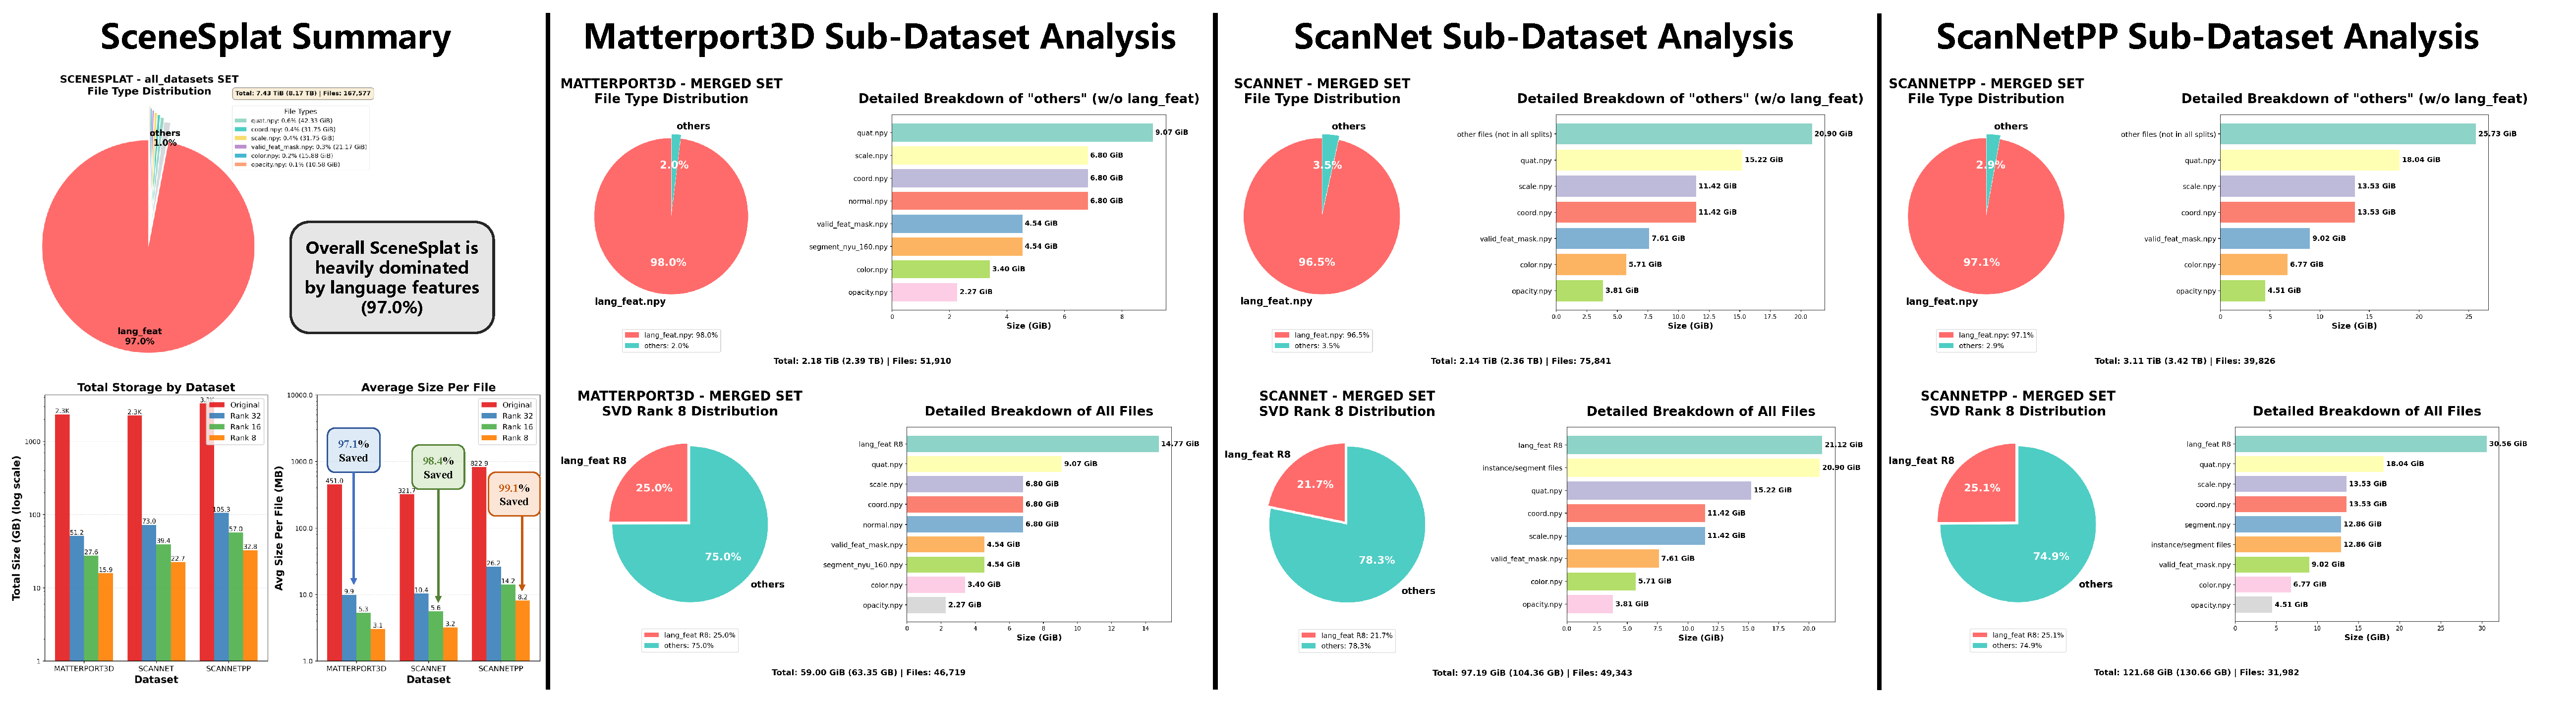
\includegraphics[width=\textwidth]{figs/Statistics.pdf}
  \caption{Storage footprint before (upper) and after (lower) feature space dimensionality reduction on SceneSplat-7k language pre-training dataset.}
  \label{fig:Dataset-Compose}
\end{figure}

\begin{table}[tb]
  \caption{Comparison of language feature storage and compressed results across datasets. We demonstrate the size of language features and the entire dataset when compressed to 8, 16, and 32 dimensions, respectively.}
  \label{tab:storage_comparison}
  \centering
  \resizebox{\textwidth}{!}{
  \begin{tabular}{@{}l|l|ccc|c@{}}
    \toprule
    Metric & Methods 
    & Matterport3D & ScanNet++ & ScanNet & SceneSplat-7k (All) \\
    \midrule
    \multirow{4}{*}{\textbf{LangFeat(GB)}} 
        & Original & 2341.20 & 3310.64 & 2267.69 & 7919.52 \\
        & Ours-rank8 & 15.85(\textcolor{blue}{$0.68\%$}) & 32.81(\textcolor{blue}{$0.99\%$}) & 22.67(\textcolor{blue}{$1.00\%$}) & 71.34(\textcolor{blue}{$0.90\%$}) \\
        & Ours-rank16 & 27.64(\textcolor{blue}{$1.18\%$}) & 56.98(\textcolor{blue}{$1.72\%$}) & 39.44(\textcolor{blue}{$1.74\%$}) & 124.07(\textcolor{blue}{$1.57\%$}) \\
        & Ours-rank32 & 51.22(\textcolor{blue}{$2.19\%$}) & 105.33(\textcolor{blue}{$3.18\%$}) & 72.97(\textcolor{blue}{$3.22\%$}) & 229.52(\textcolor{blue}{$2.90\%$}) \\
    \midrule
    \multirow{4}{*}{\textbf{Total(GB)}} 
        & Original & 2392.76 & 3417.11 & 2355.27 & 8165.14 \\
        & Ours-rank8 & 67.41 & 139.28 & 110.25 & 316.94 \\
        & Ours-rank16 & 79.20 & 163.45 & 127.02 & 369.67 \\
        & Ours-rank32 & 102.78 & 211.80 & 160.55 & 475.13 \\
    \bottomrule
  \end{tabular}}
\end{table}

% 我们提出(a) Feature Compression Pipeline 用于压缩高维度的3D语言特征矩阵，以及(b) Grid-Guided Density-Invariant Learning，用于监督模型对于不同密度输入的输出一致性。
\begin{figure}[tb]
  \centering
  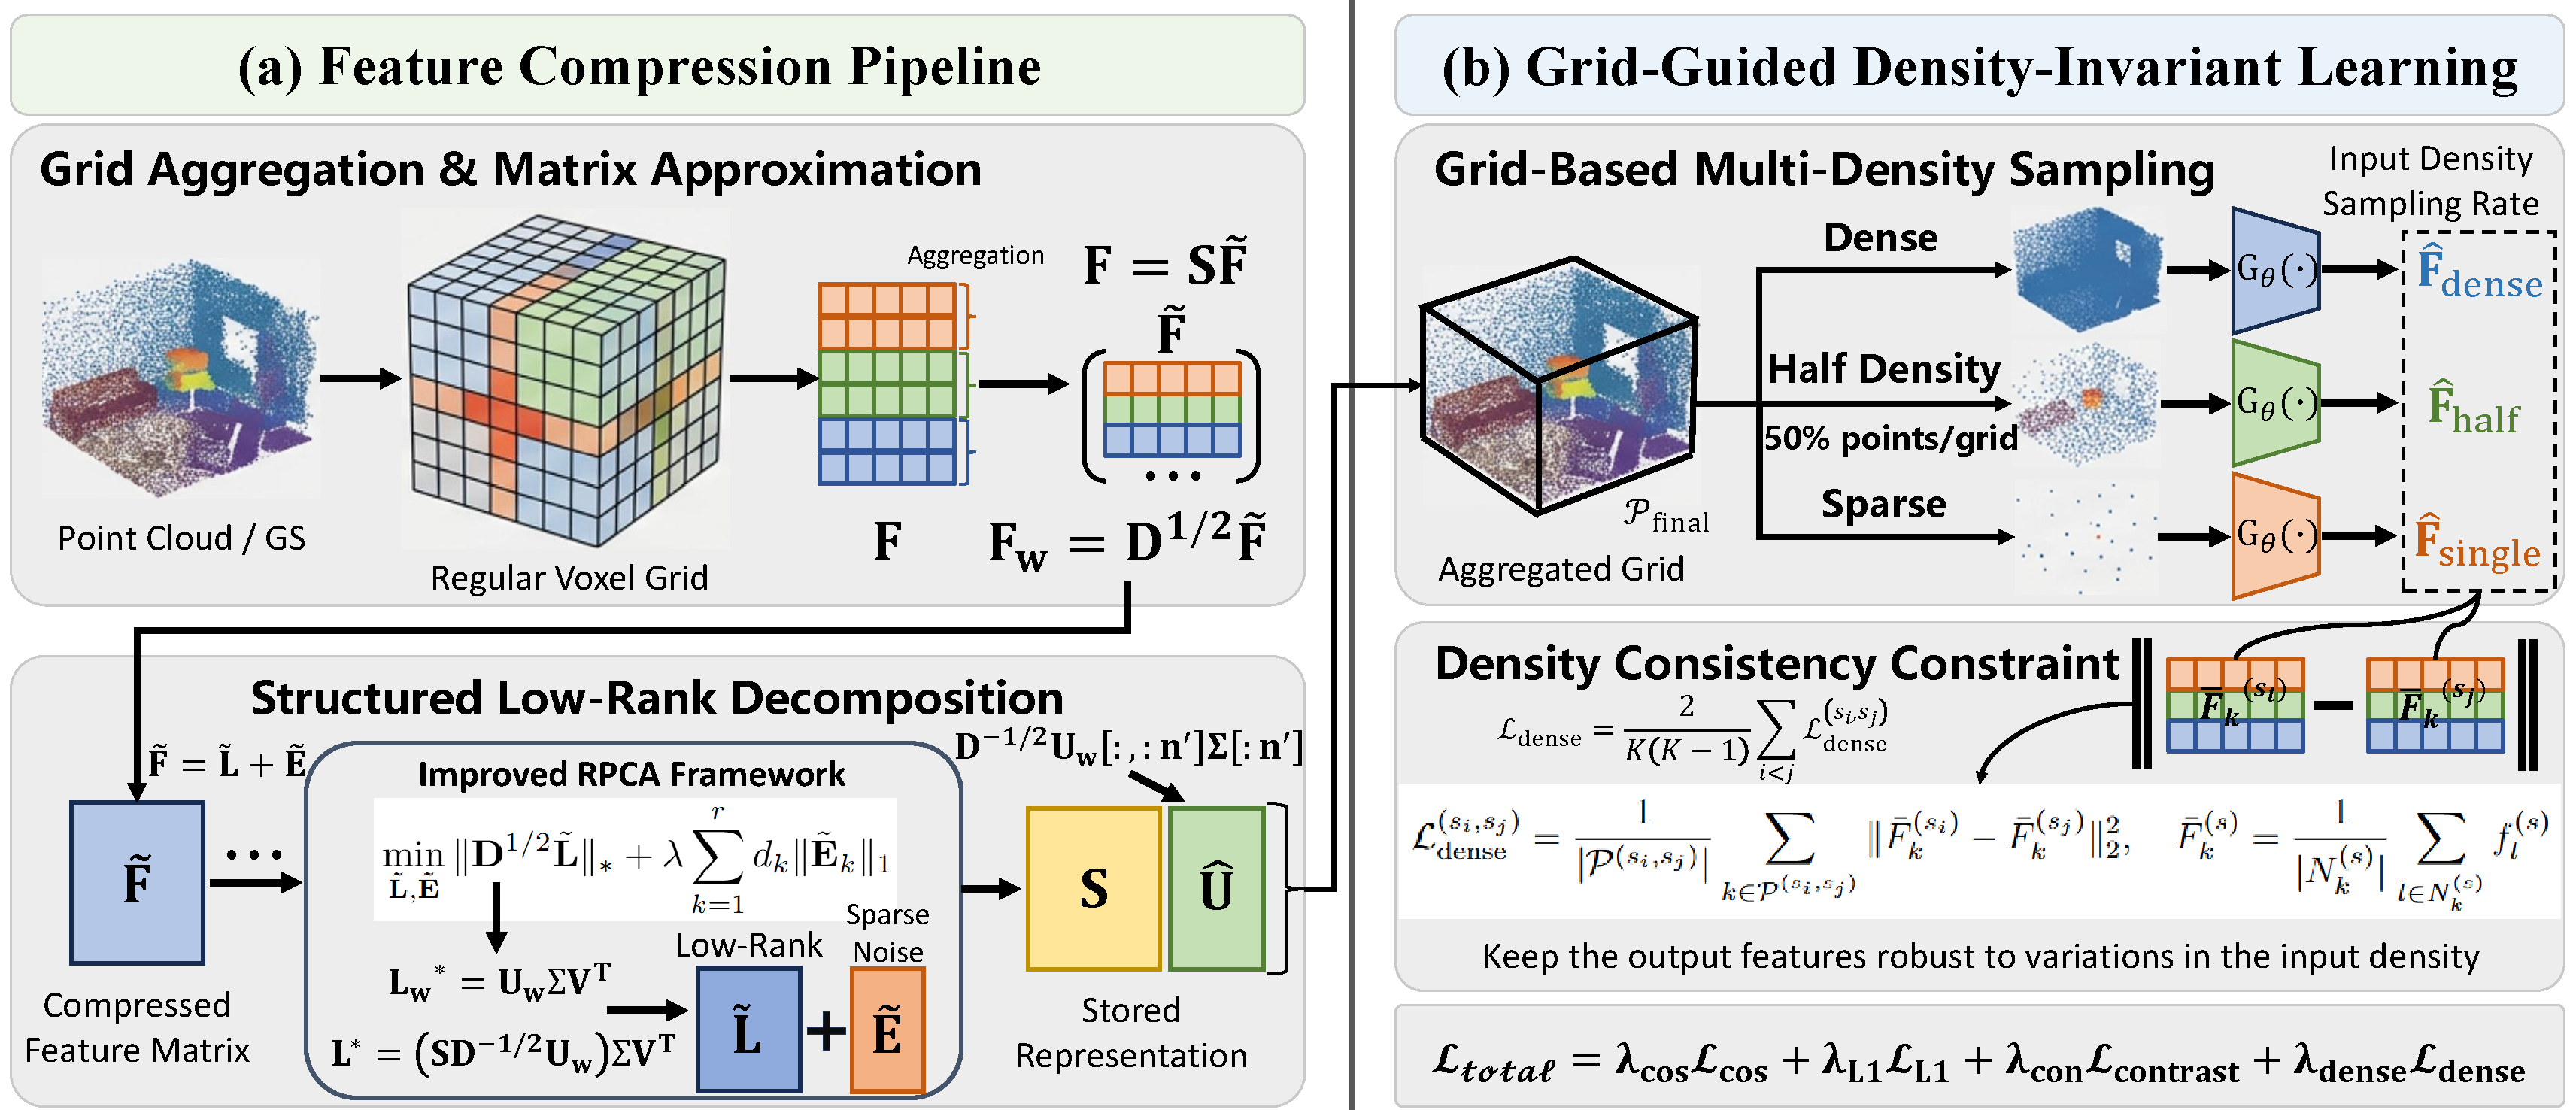
\includegraphics[width=\textwidth]{figs/Method.pdf}
  \caption{\textbf{Overview.} We introduce \textbf{(a)} a Feature Compression Pipeline to eliminate redundancy in 3D language features, and \textbf{(b)} Grid-Guided Density-Invariant Learning for robust, density-agnostic representations.}
  \vspace{-3.2em}
  \label{fig:Method}
\end{figure}

\section{Related Work}
\label{sec:related}

\subsection{Open Vocabulary Scene Understanding}
% 近年来，开放词汇模型的进展显著扩展了视觉-语言理解的能力。基础模型[81, 43, 26, 52, 49, 80, 65]实现了大规模的视觉特征提取，有效支持检测、分割等任务。为将这一能力延伸至3D领域，研究者通过将2D视觉-语言特征嵌入3D场景表示来实现开放词汇理解。早期基于NeRF的先行工作（如LERF[14, 24]和OpenNeRF[6]）采用CLIP[29]嵌入和对齐像素的特征，虽支持开放词汇查询，但因NeRF[21]本身计算密集，面临可扩展性和效率瓶颈。因此，后续研究重点转向了更高效的3D高斯泼溅（3DGS）框架[23, 30, 40, 42]。
Recent advances in open-vocabulary models have significantly advanced vision-language understanding. Foundation models \cite{big_vision,zhai2023sigmoid,radford2021learning,ravi2024sam2,kirillov2023segany,oquab2023dinov2,zhang2022dino} enable large-scale visual feature extraction, supporting tasks like detection and segmentation. To extend these capabilities to 3D, researchers embed 2D vision-language features into 3D scene representations for open-vocabulary understanding. Early NeRF-based methods, such as LERF \cite{lerf2023,rashid2023language} and OpenNeRF \cite{engelmann2024opennerf}, used CLIP \cite{radford2021learning} embeddings and pixel-aligned features to enable open-vocabulary queries. However, due to the high computational cost of NeRF \cite{mildenhall2020nerf}, they face scalability and efficiency limitations. This has shifted research focus toward the more efficient 3D Gaussian Splatting framework \cite {kerbl3Dgaussians, shi2024language, zhou2024feature, zuo2025fmgs}.

% 现有3DGS方法主要沿4个方向发展：
Existing 3DGS-based methods primarily evolve along four directions:
% 基于单场景优化的方法最先出现，其核心是将2D特征注入3DGS并针对每个场景进行优化。例如，LangSplat[27, 47]利用SAM[15]提取多层CLIP特征，再通过自编码器降维以构建紧凑的3D语言场；Feature3DGS[40]则使用卷积神经网络（CNN）提升特征维度。这些方法旨在压缩监督信号，但降维不可避免导致信息损失。另一类方法（如GOI[28]和CCL-LGS[35]）采用单一可训练特征码本存储语言嵌入，通过MLP预测渲染出的2D特征图的离散码本索引，实现了空间上的语义压缩并保留了丰富性，但其性能仍受限于对2D渲染特征图的依赖。
Per-scene optimization methods first inject and optimize 2D features per scene, often employing dimensionality reduction which leads to information loss \cite{qin2024langsplat, zhou2024feature, guo2024semantic, qu2024goi, peng2023openscene, wu2024opengaussian, zuo2025fmgs}. Other approaches use a trainable codebook for spatial compression to preserve semantics, but their 3D understanding remains limited by a reliance on 2D rendering \cite{qu2024goi,li2025instancegaussian,tian2025ccl}.
% 基于语义聚类的方法引入了显式的离散分组步骤作为先验语义结构。这类方法先将3D高斯聚合成有语义的簇（通常对应物体或部件），再为每个簇整体分配语言特征[11,17,19,25,28,37]。例如，OpenGaussian[37]基于空间邻近性和特征相似性进行由粗到细的聚类；SuperGSeg[19]和InstanceGaussian[17]则利用神经高斯建模实例级特征——前者将高斯聚合成“超级高斯”以便分配语言，后者直接为簇分配融合的语义特征；VoteSplat[11]和OpenSplat3D[25]旨在缓解直接蒸馏带来的像素级歧义。此类方法生成的簇图结构支持更高级的推理[19,39]，但通常依赖复杂的三阶段流程，增加了计算复杂度，且因整簇共享同一特征而丢失细粒度细节。
Semantic clustering methods introduce explicit discrete grouping as a prior structure, aggregating 3D Gaussians into semantic clusters (e.g., objects or parts) and assigning a shared language feature to each cluster \cite{jiang2025votesplat,li2025instancegaussian,liang2024supergseg,piekenbrinck2025opensplat3d,qu2024goi,wu2024opengaussian}. These cluster graphs enable higher-level reasoning \cite{liang2024supergseg,zhan2025hi}, but often rely on multi-stage pipelines that increase complexity and lose fine-grained details due to feature sharing.
% 免-单场景优化的方法进一步追求极致效率，致力于绕过耗时的每场景优化或聚类过程。例如，Occam‘s LGS[3, 9]、LUDVIG[38]、梯度加权3DGS[20]以及Dr.Splat[12]采用特征提升或直接注入技术，将所有2D特征投影到3DGS中，从而将计算时间从数小时大幅减少到数秒，在免训练状态下实现快速、准确的开放词汇分割。然而，这类直接特征聚合方法往往不加区分地将2D特征传播给每条相机光线相交的每个高斯，可能忽略场景的几何结构与遮挡关系。
Optimization-free methods bypass per-scene optimization or clustering for extreme efficiency. Approaches like  \cite{cheng2024occamslgssimpleapproach,drsplat25,marrie2025ludvig} project all 2D features into 3DGS \cite{kerbl3Dgaussians} via direct injection, enabling fast open-vocabulary segmentation in seconds without training, but may neglect scene geometry by uniformly propagating features along rays \cite{wang2025vala}.
% 通用化方法则寻求在新场景上实现快速、强大的开放词汇理解。其中，SceneSplat[29]是首个通用化的语言高斯泼溅方法，它直接在3D数据上进行训练和评估，在新场景上实现了显著更快的推理速度，并取得了性能上的重大提升。然而，这类方法依赖大量3D语言预训练数据，这占用了大量存储空间，严重限制了训练和推理效率。因此，我们提出SceneSplat-Compact数据集，在不损失特征质量的条件下大幅压缩存储需求，实现了更高效的训练和推理。
Generalizable approaches aim to achieve fast and robust open‑vocabulary understanding on novel scenes. For instance, SceneSplat \cite{li2025scenesplat}, the first generalizable LGS method, is trained directly on 3D data and delivers rapid inference with strong performance. However, its reliance on massive 3D language‑pretraining data incurs high storage costs and limits efficiency. To address this, we introduce SceneSplat‑Compact, a highly compressed dataset that drastically reduces storage while preserving feature quality, enabling more efficient training \& inference.
\subsection{Learning Compressed Features for Model Compression}
% 在模型压缩领域，基于特征的压缩范式因其直接作用于模型激活而非权重矩阵而受到广泛关注。该方向的开创性研究指出，Transformer架构中的特征（激活）呈现显著的低秩特性，而权重矩阵本身并不低秩，这为直接压缩权重矩阵的传统低秩近似方法提供了重要的理论反思 [Compressing Transformers: Features Are Low-Rank, but Weights Are Not!]。后续工作进一步从理论上论证了对激活进行结构化截断相较于权重压缩的优越性，并提出了可微分的奇异值分解框架，以实现自适应的压缩结构学习 [DOBI‑SVD: DIFFERENTIABLE SVD FOR LLM COMPRESSION AND SOME NEW PERSPECTIVES]。
In model compression, feature‑based methods have gained prominence by targeting model activations instead of weights. Foundational work shows that Transformer activations are intrinsically low‑rank, while the weight matrices are not, challenging traditional low‑rank weight approximation \cite{yu2023compressing}. Later research further establishes the advantage of truncating activations over compressing weights, and introduces a differentiable SVD framework for adaptive compression \cite{wang2025dobi}.
% 近年来，这一范式得到了多维度的拓展与深化。在低秩分解方向，研究重点转向了更精细的联合分解与动态机制。例如，对注意力模块中Q,K,V权重的联合低秩分解能有效减少键值缓存 [QSVD]；层选择性压缩机制能动态识别并压缩冗余矩阵，与非结构化剪枝协同工作 [LS‑PRISM]；而嵌套的、感知激活的分解方法则通过管理异常值提升了逼近精度 [NSVD]。在高效微调与适配方面，将低秩适配器与动态稀疏化相结合，能在保持参数效率的同时增强模型能力 [LoSA]。混合压缩框架的探索也日益活跃，例如统一的后训练量化与低秩压缩框架支持对多种模型架构进行可配置的压缩 [UniQL]；而通过在层级间共享权重并添加低秩差分矩阵，可以大幅降低内存占用 [DeltaLLM]。此外，面向高效推理的预训练压缩方法，通过嵌入式的上下文压缩技术，为长序列处理提供了新的解决方案 [PCC]。
Recent work extends the paradigm in multiple directions. For low‑rank decomposition, methods employ refined joint factorizations and dynamic mechanisms, such as jointly decomposing attention Q,K,V matrices to reduce KV‑cache \cite{wang2025qsvd} and using activation‑aware decomposition to handle outliers \cite{tsitsikas2020nsvd}. Hybrid frameworks that unify quantization with low‑rank compression also advance. \cite{chiang2025uniql,mikaelyan2025deltallm}.

% 然而，目前还没有将低秩分解技术应用于大规模3DGS预训练语言特征的工作。同时，尽管已经有部分工作尝试使用稀疏表示[LangSplatV2]、字典学习[OpenGaussian]、特征降维[OccamLGS]以及量化[Dr. Splat]等技术路径提升效率，针对3D开放词汇语言特征的通用压缩表示仍有待探索。
% 据我们所知，我们是首个将低秩分解技术应用于3D开放词汇语言特征的通用压缩表示的工作。
Low‑rank decomposition has not been applied to large‑scale 3DGS pretrained language features. Meanwhile, methods like sparse representation \cite{li2025langsplatv2}, dictionary learning \cite{wu2024opengaussian}, feature dimensionality reduction \cite{cheng2024occamslgssimpleapproach}, and quantization \cite{drsplat25} have been explored for efficiency, yet a general compression scheme for 3D open‑vocabulary language features remains an open problem.

\section{Method}
\label{sec:method}
\subsection{Preliminary and Definition}
\noindent\textbf{Singular Value Decomposition.} Singular Value Decomposition is a fundamental matrix factorization technique that generalizes the eigen-decomposition to non-square matrices\cite{SVD}. It decomposes any real or complex matrix $A$ into an orthogonal matrix $U$, a diagonal matrix $\Sigma$, and the transpose of another orthogonal matrix $V^T$. The core formula is $A = U \Sigma V^T$.
% \begin{equation}
% A = U \Sigma V^T
% \end{equation}
% The columns of $U$ and $V$ are the left and right singular vectors, respectively, while the diagonal entries of $\Sigma$ are the singular values, which represent the "importance" or "energy" of each component. This decomposition is crucial for applications like dimensionality reduction, noise filtering, and solving linear systems, as it provides the best low-rank approximation of the original matrix.
where $U,V$ are the singular vectors, and the diagonal entries of $\Sigma$ are the singular values. 
% This decomposition is essential for tasks such as dimensionality reduction and noise filtering, as it yields the optimal low‑rank approximation of the matrix.

\noindent\textbf{Robust Principal Component Analysis.} Robust Principal Component Analysis (RPCA) is a powerful matrix decomposition technique\cite{RPCA}, the core objective of which is to decompose a given observed data matrix $M \in \mathbb{R}^{m \times n}$ into two components: a low‑rank matrix $L$ that captures the intrinsic global structure of the data, and a sparse matrix $E$ representing noise, outliers, or specific corruptions. Its basic model can be expressed as: $M=L+E$.
% \begin{equation}
%     M=L+E
% \end{equation}

\begin{equation}
    \min_{L, E} \operatorname{rank}(L) + \lambda \|E\|_0 \quad \text{s.t.} \quad M = L + E \label{eq:RPCA-origin}
\end{equation}
RPCA recasts the original NP‑hard problem into a tractable convex relaxation

\begin{equation}
    \min_{L, E} \|L\|_* + \lambda \|E\|_1 \quad \text{s.t.} \quad M = L + E \label{eq:RPCA-approx}
\end{equation}
Here, $\lambda > 0$ is a regularization parameter that balances the trade-off between the low-rank and sparse components.
This is commonly solved via the Augmented Lagrangian Multiplier (ADMM) method:
\begin{equation}
    \mathcal{L}(L, E, Y, \mu) = \|L\|_* + \lambda \|E\|_1 + \left\langle Y, M - L - E \right\rangle + \frac{\mu}{2} \|M - L - E\|_F^2 \label{eq:RPCA-lagrange}
\end{equation}
where $Y \in \mathbb{R}^{m \times n}$ denotes the Lagrange multiplier matrix, $\mu > 0$ is the penalty parameter, $\langle \cdot, \cdot \rangle$ represents inner product, and  $\|\cdot\|_F$ stands for Frobenius norm.

\subsection{Grid‑based Feature Approximation}
% LERF与3DOVS数据集上的Grid内特征相似度分析。我们计算了原始SceneSplat的768维语言特征以及通过SVD压缩到16维后特征的L1、L2距离以及余弦相似度等指标，所有场景中的Grid内特征间都具有很高的相似度，说明了语言特征矩阵在空间维度上的冗余性。
\begin{table}[tb]
  \caption{Analysis of feature similarity within grids on the LERF and 3DOVS datasets. We compute metrics such as L1, L2 distance, and cosine similarity for both the original 768‑dim SceneSplat language features and the corresponding features compressed to 16 dimensions via SVD. High similarity is consistently observed within grids across all scenes, indicating substantial spatial redundancy in the language feature matrix.}
  \label{tab:gridsim}
  \centering
  \resizebox{\textwidth}{!}{
  \begin{tabular}{@{}l|c|cccc|ccccc|c@{}}
    \toprule
    % 表头行：用 \multicolumn 覆盖竖线
    \multicolumn{1}{c}{\multirow{2}{*}{Setting}} & \multicolumn{1}{c}{\multirow{2}{*}{Metrics}} & \multicolumn{4}{c}{LERF} & \multicolumn{5}{c}{3D-OVS} & \multicolumn{1}{c}{\multirow{2}{*}{Avg}}\\
    \cmidrule(lr){3-6} \cmidrule(lr){7-11}
    \multicolumn{1}{c}{} & & Ramen & Figurines & Teatime & Kitchen & Bed & Bench & Room & Sofa & Lawn & \\
    \midrule
    & L1 & 1.7299 & 1.8044 & 1.9874 & 2.4004 & 0.4819 & 1.3564 & 0.7954 & 1.6470 & 1.1471 & 1.4833\\
    origin & L2 & 0.0822 & 0.0855 & 0.0940 & 0.1135 & 0.0223 & 0.0638 & 0.0373 & 0.0783 & 0.0530 & 0.0700\\
    & Cos & 0.9943 & 0.9935 & 0.9923 & 0.9895 & 0.9993 & 0.9964 & 0.9985 & 0.9927 & 0.9976 & 0.9949\\
    \midrule
    & L1 & 0.1577 & 0.1400 & 0.1768 & 0.1806 & 0.0497 & 0.1605 & 0.0802 & 0.1576 & 0.1327 & 0.1373\\
    SVD-16D & L2 & 0.0501 & 0.0446 & 0.0577 & 0.0577 & 0.0168 & 0.0523 & 0.0256 & 0.0546 & 0.0454 & 0.0450\\
    & Cos & 0.9975 & 0.9976 & 0.9964 & 0.9965 & 0.9995 & 0.9972 & 0.9991 & 0.9949 & 0.9981 & 0.9974\\
    \bottomrule
  \end{tabular}}
\end{table}

% 之前的工作仅关注针对完整数据矩阵的压缩，忽略了某些低秩矩阵的固有特性。例如，开放词汇场景理解中的3D语言特征矩阵，其行与行之间的特征往往是相似的，这是因为在稠密点云条件下，空间中相邻的两个点往往对应相同的语义。由此，我们假设空间上相邻的两个点具有近似相同的语言特征。
% Existing research has predominantly concentrated on compressing the complete data matrix, while neglecting the inherent characteristics of certain low‑rank structures. In open‑vocabulary scene understanding, for example, the 3D language feature matrix demonstrates strong inter‑row similarity, owing to the fact that neighboring points in dense point clouds commonly share the same semantic label. This observation motivates the hypothesis that spatially adjacent points exhibit nearly equivalent language features.
Existing work typically compresses the full data matrix, often overlooking its inherent low‑rank structure. In open‑vocabulary scene understanding, for instance, the 3D language‑feature matrix exhibits strong row‑wise similarity because neighboring points in a dense cloud usually share the same semantic label. We therefore observe that spatially adjacent points have nearly identical language features.

% 如何判断两个点在空间中相邻？参考PTV3的点云序列化流程，我们将同一个Grid内的点云视为相邻，且具有相同serialized encoding。具体而言，将3D点云坐标p归一化后除以网格大小g并向下取整，得到离散化的整数网格坐标p/g，随后映射到特定space-filling curve上的序列化编码\phi^{-1}(p/g).
% 然而，离散化后的网格中很大一部分只含一个点云，称为稀疏网格。为了进一步聚合并压缩相似的点云特征，我们提出一种基于余弦相似度的网格聚合策略。具体而言，针对每个稀疏网格p_i \in \mathcal{P}_{sparse}，我们选出与其距离最近的k个网格\mathcal{P}_{k}，随后于每个网格的平均语言特征计算余弦相似度，选择相似度最高的网格进行合并。
% How can we determine whether two points are spatially adjacent? Following the point cloud serialization procedure of PTv3\cite{wu2024ptv3,wu2022ptv2,wu2024ppt,pointcept2023}, we consider points belonging to the same grid as neighbors and assign them identical serialized encoding. Specifically, after normalizing the 3D point cloud $\mathcal{X} \in \mathbb{R}^{N \times 3}$, we divide it by the grid size $g \in \mathbb{R}$ and take the floor to obtain the discretized integer grid coordinate $\lfloor \mathbf{x}_i/g \rfloor \in \mathbb{R}^{3}$. This coordinate is then mapped to a serialized encoding $\varphi^{-1}(\lfloor \mathbf{x}_i/g \rfloor)$ on a specific space‑filling curve.
% However, a large portion of the discretized grids contain only a single point cloud, referred to as sparse grids. To further aggregate and compress similar point cloud features, we introduce a similarity‑based grid merging strategy. Specifically, for each sparse grid $p_i \in \mathcal{P}_\text{sparse}^i$, we first select the k nearest neighboring grids $\mathcal{P}_k^i$ in spatial distance. Then, we compute the cosine similarity between the average language features of $p_i$ and each grid in $\mathcal{P}_k$, and merge $p_i$ with the grid $p_*$ that yields the highest similarity.

To identify spatially adjacent points, we adopt the point‑cloud serialization of PTv3 \cite{wu2024ptv3,wu2022ptv2,wu2024ppt,pointcept2023}. Points that fall into the same grid are treated as neighbors and share the same serialized code. Concretely, after normalizing the point cloud $\mathcal{X} \in \mathbb{R}^{N \times 3}$, we discretize it by the grid size $g \in \mathbb{R}$ and take the floor to obtain integer grid coordinates $\lfloor \mathbf{x}_i/g \rfloor \in \mathbb{R}^{3}$.
Many of the resulting grids, however, contain only a single point, called sparse grids. To aggregate them, we introduce a similarity‑based merging strategy. For each sparse grid $p_i \in \mathcal{P}_\text{sparse}^i$, we first find its k nearest neighboring grids $\mathcal{P}_k^i$ in spatial distance, then compute the cosine similarity between the average language features of $p_i$ and each grid in $\mathcal{P}_k^i$, and finally merge $p_i$ with the grid $p_*$ that achieves the highest similarity.

\begin{equation}
    \mathcal{P}_k^i = \underset{p_j \in \mathcal{P},\, |\mathcal{P}_k|=k}{\arg\min} \|p_j - p_i\|_2, \quad p_j = \lfloor \mathbf{x}_j/g \rfloor
\end{equation}

\begin{equation}
    p_* = \underset{p_j \in \mathcal{P}_k^i} {\arg\max} \text{ sim}(p_i, p_j), \quad\text{sim}(p_i, p_j) = \frac{\bar{\mathbf{f}}_i \cdot \bar{\mathbf{f}}_j}{\|\bar{\mathbf{f}}_i\| \|\bar{\mathbf{f}}_j\|}
\end{equation}
where $\bar{\mathbf{f}_i} = \frac{1}{N_i} \sum_{j=1}^{N_i} \mathbf{f}_j$ denotes the average language feature of all point clouds within grid $p_i$, and $N_i$ denotes the number of point clouds in $p_i$. 
% 当p_i与p_*合并后，新的网格将加入含多个点云的网格集合，随后继续遍历\mathcal{P}_\text{sparse}^i，直至所有稀疏网格都被合并到其他网格中。最后，将每个网格内的语言特征替换为该网格的平均语言特征，得到原始语言特征矩阵F的近似F'。整套流程可以概括为算法1.
After $p_i$ is merged with $p_*$, the new grid is added to the set of grids containing multiple point clouds. Then, the traversal of $\mathcal{P}_\text{sparse}^i$ continues until all sparse grids have been merged into others. 

Finally, the language features within each grid are replaced by the average language feature $\bar{\mathbf{f}_i'}$, yielding an approximation $\tilde{\mathbf{F}}$ of the original language feature matrix $\mathbf{F}$. The overall pipeline is summarized in Algorithm \ref{alg:algorithm}.
\begin{equation}
    \tilde{\mathbf{F}} = [\bar{\mathbf{f}}_1';\bar{\mathbf{f}}_2';\dots;\bar{\mathbf{f}}_{N'}']^T
\end{equation}

% 我们在LERF与3DOVS数据集上分析了网格化特征聚合算法后，在将所有语言特征近似为平均特征之前，每个Grid内对应的平均特征相似度指标，如表x所示。所有场景的平均余弦相似度都接近1，且具有较小的平均L2距离。在执行SVD分解并压缩到16维特征矩阵后，Grid内特征相似度还有进一步显著提升。这验证了3D语言特征矩阵的行间是高度冗余的。
We analyze the average feature similarity metrics within each grid on the LERF\cite{lerf2023} and 3DOVS\cite{liu2023weakly} datasets after applying the grid‑based feature aggregation algorithm, before approximating all language features with the grid averages. The results are shown in Table \ref{tab:gridsim}. The average cosine similarity across all scenes is close to 1, accompanied by a small mean L2 distance. After performing SVD and compressing to a 16‑dimensional feature matrix, the intra‑grid feature similarity exhibits a further significant improvement. The results validate that rows of the 3D language feature matrix are highly redundant.

\begin{algorithm}[tb]
\caption{Grid feature aggregation.}
\label{alg:algorithm}
% \textbf{Input}: Point clouds $x$, Language feature matrix $\mathbf{F}$.\\
% \textbf{Parameter}: Grid size $g$, Nearest‑neighbor search radius $k$\\
% \textbf{Output}: Approximate language feature matrix $\tilde{\mathbf{F}}$
\begin{algorithmic}[1] %[1] enables line numbers
\Require Point clouds $\mathcal{X}$, language feature matrix $\mathbf{F}$, grid size $g$, nearest‑neighbor search radius $k$
\Ensure Approximate language feature matrix $\tilde{\mathbf{F}}$

\State \textbf{Phase 1: Voxelization with Iterative Feature Averaging}
\State Initialize $N_p \gets 0$, $\bar{\mathbf{f}}_p \gets \mathbf{0}$ \Comment{Initialize count and average}
\State Initialize $\mathcal{P}_{\text{dense}} \gets \emptyset$, $\mathcal{P}_{\text{sparse}} \gets \mathcal{P}$ \Comment{Initially assign to sparse set}
\For{each point $\mathbf{x}_i \in \mathcal{X}$ with feature $\mathbf{f}_i \in \mathbf{F}$}
    \State Compute grid index: $p \gets \lfloor \mathbf{x}_i / g \rfloor$
    \State $N_p \gets N_p + 1$ \Comment{Increment count}
    \State $\bar{\mathbf{f}}_p \gets (1-1/{N_p}) \cdot \bar{\mathbf{f}}_p + \mathbf{f}_i/{N_p}$ \Comment{Iterative update of average}
    \If{$N_p = 2$} \Comment{Transition from sparse to dense when count becomes 2}
        \State $\mathcal{P}_{\text{sparse}} \gets \mathcal{P}_{\text{sparse}} \setminus \{p\}$,  $\mathcal{P}_{\text{dense}} \gets \mathcal{P}_{\text{dense}} \cup \{p\}$
    \EndIf
\EndFor

\State \textbf{Phase 2: Grid Aggregation with Iterative Feature Update}
\While{$\mathcal{P}_{\text{sparse}}$ is not empty}
    \State Pick a sparse grid $p_i \in \mathcal{P}_{\text{sparse}}$
    \State Find $k$ nearest neighbors $\mathcal{P}_k^i \subset \mathcal{P}$ of $p_i$
    \State $p_* \gets \arg\max_{p_j \in \mathcal{P}_k^i} \text{sim}(\bar{\mathbf{f}}_{p_i}, \bar{\mathbf{f}}_{p_j})$
    \State $N_{p_*} \gets N_{p_*} + 1$ \Comment{\textbf{Merge} $p_i$ into $p_*$}
    \State $\bar{\mathbf{f}}_{p_*} \gets (1 - 1/N_{p_*}) \cdot \bar{\mathbf{f}}_{p_*} + \bar{\mathbf{f}}_{p_i} / N_{p_*}$ \Comment{Iterative merge update}
    \State $\mathcal{P}_{\text{sparse}} \gets \mathcal{P}_{\text{sparse}} \setminus \{p_i\}$, $\mathcal{P}_{\text{dense}} \gets \mathcal{P}_{\text{dense}} \cup \{p_*\}$ \Comment{Mark $p_i$ as merged}
    \If{$p_* \in \mathcal{P}_{\text{sparse}}$}
        \State $\mathcal{P}_{\text{sparse}} \gets \mathcal{P}_{\text{sparse}} \setminus \{p_*\}$
    \EndIf
\EndWhile

\State \textbf{Phase 3: Output Feature Assignment}
\For{each grid $p$ in $\mathcal{P}_{\text{dense}}$}
    \For{each point $\mathbf{x}_i \in p$}
        \State Assign average feature: $\tilde{\mathbf{f}}_i \gets \bar{\mathbf{f}}_p$
    \EndFor
\EndFor

\State Construct $\tilde{\mathbf{F}}$ from all $\tilde{\mathbf{f}}_i$
\State \Return $\tilde{\mathbf{F}}$

\end{algorithmic}
\end{algorithm}


\subsection{Structured RPCA}
% 在验证了特征矩阵的冗余性后，我们通过网格化特征聚合算法，以F'近似F实现矩阵压缩。值得注意的是，空间维度上的压缩并不影响F'在特征维度上的冗余，可以进一步通过SVD压缩F'的特征。然而，聚合算法改变了矩阵F的奇异值。因此，本节将探究F与F'间奇异值分解的关系，并将其应用到RPCA算法中，以进一步实现F'在特征维度上的压缩。
% After verifying the redundancy of the feature matrix, we employ the grid‑based feature aggregation algorithm to approximate $\mathbf{F}$ with $\tilde{\mathbf{F}}$, thereby compressing the matrix. Notably, compression along the spatial dimension does not eliminate the redundancy of $\tilde{\mathbf{F}}$ along the feature dimension, which can be further compressed via SVD. However, the aggregation algorithm alters the singular values of matrix $\mathbf{F}$. Thus, this section investigates the relationship between the singular value decompositions of $\mathbf{F}$ and $\tilde{\mathbf{F}}$, and applies it to the RPCA framework to achieve additional compression of $\tilde{\mathbf{F}}$ in the feature dimension.
After confirming the redundancy of the feature matrix, we first apply grid‑based aggregation to spatially compress $\mathbf{F}$ into $\tilde{\mathbf{F}}$. While this reduces spatial redundancy, $\tilde{\mathbf{F}}$ remains redundant along the feature dimension and can be further compressed via SVD. However, the aggregation changes the singular values of the original matrix. We therefore analyze the relationship between the SVDs of $\mathbf{F}$ and $\tilde{\mathbf{F}}$, and incorporate this insight into an RPCA framework to achieve additional, structured compression in the feature dimension.

% 我们首先分析矩阵奇异值分解的变化。
We begin by analyzing how the singular value decomposition of the matrix changes. Let $\mathbf{A} \in \mathbb{R}^{m \times n}$ be the original matrix containing duplicate rows, and let  $\tilde{\mathbf{A}} \in \mathbb{R}^{r \times n}, r \leq m$ be the matrix composed of all its distinct rows. Define a selection matrix  $S \in \{0,1\}^{m \times r}$ such that:
\begin{equation}
    \mathbf{A} = \mathbf{S} \tilde{\mathbf{A}}, \quad\sum_{j=1}^{r} \mathbf{S}_{ij} = 1, \text{ for } \forall i = 1,\ldots,m
    \label{eq:3.31}
\end{equation}
where each row of the selection matrix $\mathbf{S}$ is a one-hot vector. We further define the diagonal weight matrix $\mathbf{D} \in \mathbb{R}^{r \times r}$ as:
\begin{equation}
    \mathbf{D} = \mathbf{S}^T \mathbf{S} = \operatorname{diag}(d_1, d_2, \ldots, d_r)
    \label{eq:3.32}
\end{equation}
where $d_j$ denotes the number of occurrences of the j-th row of $\tilde{\mathbf{A}}$ in $\mathbf{A}$. Then construct the weighted matrix $\mathbf{A}_w \in \mathbb{R}^{r \times n}$: 
% \begin{equation}
%     \mathbf{A_w} = \mathbf{D}^{1/2} \tilde{\mathbf{A}}
%     \label{eq:3.33}
% \end{equation}
\begin{equation}
    \mathbf{A_w} = \mathbf{D}^{1/2} \tilde{\mathbf{A}}, \quad \mathbf{A_w}^T \mathbf{A_w} = \tilde{\mathbf{A}}^T \mathbf{D} \tilde{\mathbf{A}} = \mathbf{A}^T \mathbf{A}
    \label{eq:3.34}
\end{equation}
Consequently, $\mathbf{A}_w$ and $\mathbf{A}$ share the same Gram matrix, and thus have identical singular values. Hence, we perform the compact singular value decomposition on the weighted matrix: $\mathbf{A_w} = \mathbf{U_w} \mathbf{\Sigma} \mathbf{V}^T$. Combining Eq. \eqref{eq:3.31} \& Eq. \eqref{eq:3.34} yields the following equation:
\begin{equation}
    \mathbf{A} = \mathbf{S} \mathbf{D}^{-1/2} \mathbf{A_w} = (\mathbf{S} \mathbf{D}^{-1/2} \mathbf{U_w}) \mathbf{\Sigma} \mathbf{V}^T
    \label{eq:3.35}
\end{equation}
Let $\mathbf{U} = \mathbf{S} \mathbf{D}^{-1/2} \mathbf{U_w} \in \mathbb{R}^{m \times r}$. It can be proved that the columns of $\mathbf{U}$ are orthonormal, and thus $\mathbf{A} = \mathbf{U}\mathbf{\Sigma}\mathbf{V}^T$ is the compact SVD of $\mathbf{A}$.

% 下面分析如何将方程13应用到RPCA算法中对矩阵F进行分解。
We now analyze how Eq. \eqref{eq:3.35} can be applied to the RPCA algorithm for decomposing matrix $\mathbf{F}$. Based on the structural assumption in Eq. \eqref{eq:3.31}, we can rewrite the RPCA problem Eq. \eqref{eq:RPCA-approx} as:
\begin{equation}
    \min_{\tilde{\mathbf{L}}, \tilde{\mathbf{E}}} \|\mathbf{S} \tilde{\mathbf{L}}\|_* + \lambda \|\mathbf{S} \tilde{\mathbf{E}}\|_1 \quad \text{s.t.} \quad \tilde{\mathbf{F}} = \tilde{\mathbf{L}} + \tilde{\mathbf{E}}
    \label{eq:3.36}
\end{equation}
where $\mathbf{L} = \mathbf{S}\tilde{\mathbf{L}}$, $\mathbf{E} = \mathbf{S}\tilde{\mathbf{E}}$. Analogously, we construct the weighted matrix $\mathbf{L_w}=\mathbf{D}^{1/2} \tilde{\mathbf{L}}$. From Eq. \eqref{eq:3.34}, we know that $\mathbf{L}$ and $\mathbf{L_w}$ share the same singular values and therefore have identical nuclear norms.
\begin{equation}
    \|\mathbf{L}\|_* = \|\mathbf{L_w}\|_* = \|\mathbf{D}^{1/2} \tilde{\mathbf{L}}\|_*
    \label{eq:3.37}
\end{equation}

Given that each row of $\mathbf{S}$ contains exactly one nonzero element, we have for the L1‑norm of matrix $\mathbf{E}$:
\begin{equation}
    \|\mathbf{E}\|_1 = \sum_{i=1}^m \sum_{j=1}^n |\mathbf{E}_{ij}| = \sum_{i=1}^m \sum_{j=1}^n \left| \sum_{k=1}^r \mathbf{S}_{ik} \tilde{\mathbf{E}}_{kj} \right| = \sum_{k=1}^r d_k \|\tilde{\mathbf{E}}_{k}\|_1
    \label{eq:3.38}
\end{equation}
where $\tilde{\mathbf{E}}_{k}$ is the k-th row of $\tilde{\mathbf{E}}$, and $\|\tilde{\mathbf{E}}_{k}\|_1$ denotes the L1-norm of the row vector.

Combining Eq. \eqref{eq:3.37} and Eq. \eqref{eq:3.38}, we can transform problem Eq. \eqref{eq:3.36} into:
\begin{equation}
    \min_{\tilde{\mathbf{L}}, \tilde{\mathbf{E}}} \|\mathbf{D}^{1/2} \tilde{\mathbf{L}}\|_* + \lambda \sum_{k=1}^r d_k \|\tilde{\mathbf{E}}_{k}\|_1 \quad \text{s.t.} \quad \tilde{\mathbf{F}} = \tilde{\mathbf{L}} + \tilde{\mathbf{E}}
    \label{eq:3.39}
\end{equation}

\iffalse
\begin{algorithm}[tb]
\caption{Structured RPCA via Weighted Optimization}
\label{alg:structured_rpca}
\begin{algorithmic}[1]
\Require Distinct row matrix $\tilde{\mathbf{F}}$, selection matrix $\mathbf{S}$, regularization parameter $\lambda$, tolerance $\varepsilon$, maximum iterations $K_{\max}$
\Ensure Optimal low-rank component $\mathbf{L}^*$, optimal sparse component $\mathbf{E}^*$
\State Compute weight matrix: $\mathbf{D} \gets \mathbf{S}^T \mathbf{S}$
\State Initialize: $\tilde{\mathbf{L}}^{(0)} \gets \tilde{\mathbf{F}}$, $\tilde{\mathbf{E}}^{(0)} \gets \mathbf{0}$, $\mathbf{Y}^{(0)} \gets \mathbf{0}$, $k \gets 0$, $\mu > 0$
\State Initialize: $c \gets 0$ \Comment{Convergence flag: $0$ = not converged, $1$ = converged}

\While{$k < K_{\max}$ and $c = 0$}
    \State Store previous iterates: $\tilde{\mathbf{L}}^{\text{prev}} \gets \tilde{\mathbf{L}}^{(k)}$, $\tilde{\mathbf{E}}^{\text{prev}} \gets \tilde{\mathbf{E}}^{(k)}$
    
    \State \textbf{Update $\tilde{\mathbf{L}}$}:
    $$\mathbf{M} \gets \tilde{\mathbf{F}} - \tilde{\mathbf{E}}^{(k)} + \mathbf{Y}^{(k)}/\mu$$
    $$\tilde{\mathbf{L}}^{(k+1)} \gets \mathbf{D}^{-1/2} \mathcal{D}_{\lambda/\mu}\left(\mathbf{D}^{1/2} \mathbf{M}\right)$$
    \Comment{$\mathcal{D}_{\tau}(\mathbf{M}) = \mathbf{U} \operatorname{diag}(\max(\sigma_i - \tau, 0)) \mathbf{V}^T$}
    
    \State \textbf{Update $\tilde{\mathbf{E}}$} (row-wise):
    \For{$i = 1$ to $r$}
        $$\tilde{\mathbf{E}}^{(k+1)}[i,:] \gets \mathcal{S}_{\lambda d_i/\mu}\left(\tilde{\mathbf{F}}[i,:] - \tilde{\mathbf{L}}^{(k+1)}[i,:] + \mathbf{Y}^{(k)}[i,:]/\mu\right)$$
        \Comment{$\mathcal{S}_{\tau}(x)=\operatorname{sign}(x)\max(|x|-\tau,0)$}
    \EndFor
    
    \State \textbf{Update Lagrange multiplier}:
    \[
    \mathbf{Y}^{(k+1)} \gets \mathbf{Y}^{(k)} + \mu \left(\tilde{\mathbf{F}} - \tilde{\mathbf{L}}^{(k+1)} - \tilde{\mathbf{E}}^{(k+1)}\right)
    \]
    
    \State \textbf{Compute residuals and check convergence}:
    \State $r_p \gets \|\tilde{\mathbf{F}} - \tilde{\mathbf{L}}^{(k+1)} - \tilde{\mathbf{E}}^{(k+1)}\|_F$ \Comment{Primal residual}
    \State $r_d \gets \mu \|\tilde{\mathbf{L}}^{(k+1)} - \tilde{\mathbf{L}}^{(k)}\|_F$ \Comment{Dual residual}
    \If{$r_p < \varepsilon$ and $r_d < \varepsilon$}
        \State $c \gets 1$ \Comment{Mark as converged}
    \EndIf
    
    \State $k \gets k + 1$
\EndWhile

\State Set optimal solutions: $\tilde{\mathbf{L}}^* \gets \tilde{\mathbf{L}}^{(k)}$, $\tilde{\mathbf{E}}^* \gets \tilde{\mathbf{E}}^{(k)}$
\State Recover original-scale components: $\mathbf{L}^* \gets \mathbf{S} \tilde{\mathbf{L}}^*$, $\mathbf{E}^* \gets \mathbf{S} \tilde{\mathbf{E}}^*$
\State \Return $\mathbf{L}^*$, $\mathbf{E}^*$
\end{algorithmic}
\end{algorithm}
\fi


% 在处理实际的3D语言特征矩阵时，一般有$m>r>>n$，因此标准RPCA的计算复杂度为。相比之下，我们的结构化RPCA算法计算复杂度为，效率大约提升至原来的m/r倍。
% In practical applications involving 3D language feature matrices, the relationship typically satisfies $m > r \gg n$. Consequently, the computational complexity of standard RPCA is $O(mn \cdot min(m,n)) = O(m \cdot n^2)$, whereas that of our structured RPCA algorithm is $O(r \cdot n^2)$. This yields an efficiency improvement by approximately a factor of $m/r$.

% 此外，我们最终存储的并非低秩矩阵L_*，而是其经过SVD分解后压缩至低维的部分。具体而言，根据方程13，假设加权矩阵的SVD分解为\mathbf{L_w}^* = \mathbf{U_w} \mathbf{\Sigma} \mathbf{V}^T，则L_*的SVD分解为\mathbf{L}^* = (\mathbf{S} \mathbf{D}^{-1/2} \mathbf{U_w}) \mathbf{\Sigma} \mathbf{V}^T。因此，我们实际需要存储的数据仅为选择矩阵S以及压缩特征：
Furthermore, what we ultimately store is not the low‑rank matrix $\mathbf{L}^*$ itself, but its compressed low‑dimensional components obtained via SVD. Specifically, following Eq. \eqref{eq:3.35}, given the SVD of the weighted matrix as $\mathbf{L_w}^* = \mathbf{U_w} \mathbf{\Sigma} \mathbf{V}^T$, the SVD of $\mathbf{L}^*$ can be expressed as $\mathbf{L}^* = (\mathbf{S} \mathbf{D}^{-1/2} \mathbf{U_w}) \mathbf{\Sigma} \mathbf{V}^T$. Hence, the actual data we need to store are only the selection matrix $\mathbf{S}$ and the compressed features:
\begin{equation}
    \hat{\mathbf{U}} = \mathbf{D}^{-1/2} \mathbf{U_w}[:,:n'] \mathbf{\Sigma}[:n'] \in \mathbb{R}^{r \times n'}
     \label{eq:3.310}
\end{equation}
where $\mathbf{U_w}[:,:n']$ and $\mathbf{\Sigma}[:n']$ denote the first $n'$ columns of $\mathbf{U_w}$ and the diagonal matrix composed of the first $n'$ singular values of $\mathbf{\Sigma}$, respectively, and $n' \ll n$. \\
% 由于S的每一行都是onehot向量，因此可以压缩成一个m维度的索引向量。最终的存储量减少至：m+rn'，压缩比达到mn / (m+rn').
Since each row of $\mathbf{S}$ is one‑hot, it can be compressed into an m-dimensional index vector. As a result, the final storage is reduced to $m + rn'$, and the compression ratio reaches $mn / (m + rn')$.
Detailed derivations and the structured RPCA algorithm are provided in the supplement.

\subsection{Grid-Guided Density-Invariant Learning}
% 以往绝大部分开放词汇场景理解的工作都是以完整的点云或高斯场景为输入。然而，实际应用场景中往往对输入稠密点云下采样以提升效率。我们发现以往的前馈式方法中存在一定的对稠密点云输入的过拟合现象，当输入下采样的稀疏点云时模型的输出结果会更加不稳定。为了缓解这个问题，我们提出Grid-Guided Density-Invariant Learning以提升模型对任意密度点云输入的鲁棒性。
% Most existing works on open‑vocabulary scene understanding take a complete point cloud or Gaussian scene as input. However, in practical applications, the input dense point cloud is often downsampled to improve efficiency. We observe that previous feed‑forward approaches exhibit a certain overfitting tendency to dense point‑cloud inputs, leading to more unstable outputs when provided with down‑sampled sparse point clouds. To mitigate this issue, we propose Grid‑Guided Density‑Invariant Learning to enhance model robustness against point‑cloud inputs of arbitrary densities.
Most open‑vocabulary 3D understanding methods assume dense point‑cloud inputs, yet in practice the data are often down‑sampled for efficiency. We find that feed‑forward models tend to overfit to dense inputs, becoming unstable on sparse point clouds. To improve robustness to arbitrary input densities, we introduce Grid‑Guided Density‑Invariant Learning.

% 3.2节中的网格聚合算法已经将输入点云聚合于固定大小的网格中，这天然有利于基于网格的下采样方法。我们遍历聚合后的网格集合$\mathcal{P}_{final}$并从每个网格中分别随机采样1个点和50%的点，构成下采样点云集合$\mathcal{X}_{single}$和$\mathcal{X}_{half}$。随后，输入以\theta为参数的网络$G_{\theta}(\cdot)$中得到预测的语言特征$\hat{F} = G_{\theta}(\mathcal{X})$.由此，我们提出Grid-Aligned Cross-Density Consistency Loss以约束不同密度点云输入下预测的特征一致性。
The grid aggregation algorithm in Section 3.2 already groups the input point cloud into fixed‑size grids, which naturally lends itself to grid‑based down‑sampling. We traverse the aggregated grid set $\mathcal{P}_{\text{final}}$ and randomly sample one point from each grid to form the down‑sampled point set $\mathcal{X}_{\text{single}}$, and sample 50\% of the points from each grid to form $\mathcal{X}_{\text{half}}$. These down‑sampled sets are then fed into the network $G_{\theta}(\cdot)$ parameterized by $\theta$, yielding the predicted language features $\hat{F} = G_{\theta}(\mathcal{X})$. Let $\mathcal{S} = \{s_1, s_2, s_3\}$ denote the set of three sampling scenarios: dense, half‑density, and single‑point per‑grid. $\mathcal{P}^{(s_i,s_j)} = \mathcal{P}^{(s_i)} \cap \mathcal{P}^{(s_j)}$ denotes the set of common grids between scenarios $s_i$ and $s_j$. We compute the feature consistency loss $\mathcal{L}_{\text{dense}}^{(s_i,s_j)}$ between different sampling scenarios as follows.

\begin{equation}
    \mathcal{L}_{\text{dense}}^{(s_i,s_j)} = \frac{1}{|\mathcal{P}^{(s_i,s_j)}|} \sum_{k \in \mathcal{P}^{(s_i,s_j)}} \|\bar{F}_k^{(s_i)} - \bar{F}_k^{(s_j)}\|_2^2, \quad \bar{F}_k^{(s)} = \frac{1}{|N_k^{(s)}|} \sum_{l \in N_k^{(s)}} f_l^{(s)}
     \label{eq:loss-dense-perscene}
\end{equation}
  
\begin{equation}
    \mathcal{L}_{\text{dense}} = \frac{2}{K(K-1)} \sum_{i < j} \mathcal{L}_{\text{dense}}^{(s_i,s_j)}
\end{equation}
where $\bar{F}_k^{(s)}$ denotes the average language feature of the k-th grid in scenario $s$, $N_k^{(s)}$ is the number of point clouds, and $f_l^{(s)}$ is the l-th language feature in the k-th grid. The overall consistency constraint loss $\mathcal{L}_{\text{dense}}$ is the mean of the consistency losses between all scenario pairs. We set $K=3$ in this paper.

% 我们在Vision-Language pretraining损失的基础上增加密度一致性约束项，得到如下的训练损失函数。
On top of the Vision‑Language pretraining loss\cite{li2025scenesplat}, we incorporate a density consistency constraint, yielding the following training loss function.
\begin{equation}
    \mathcal{L}_{total} = \lambda_{cos}\mathcal{L}_{cos} + \lambda_{L1}\mathcal{L}_{L1} + \lambda_{con}\mathcal{L}_{contrast} + \lambda_{dense}\mathcal{L}_{dense}
    \label{eq:total-loss}
\end{equation}
% \section{Analysis of Language Feature Redundancy}
\section{The Language Feature is Low-Rank}
\label{sec:analysis}
% LERF 与 3DOVS数据集上的特征空间降维前后的特征分布可视化对比。
\begin{figure}[tb]
  \centering
  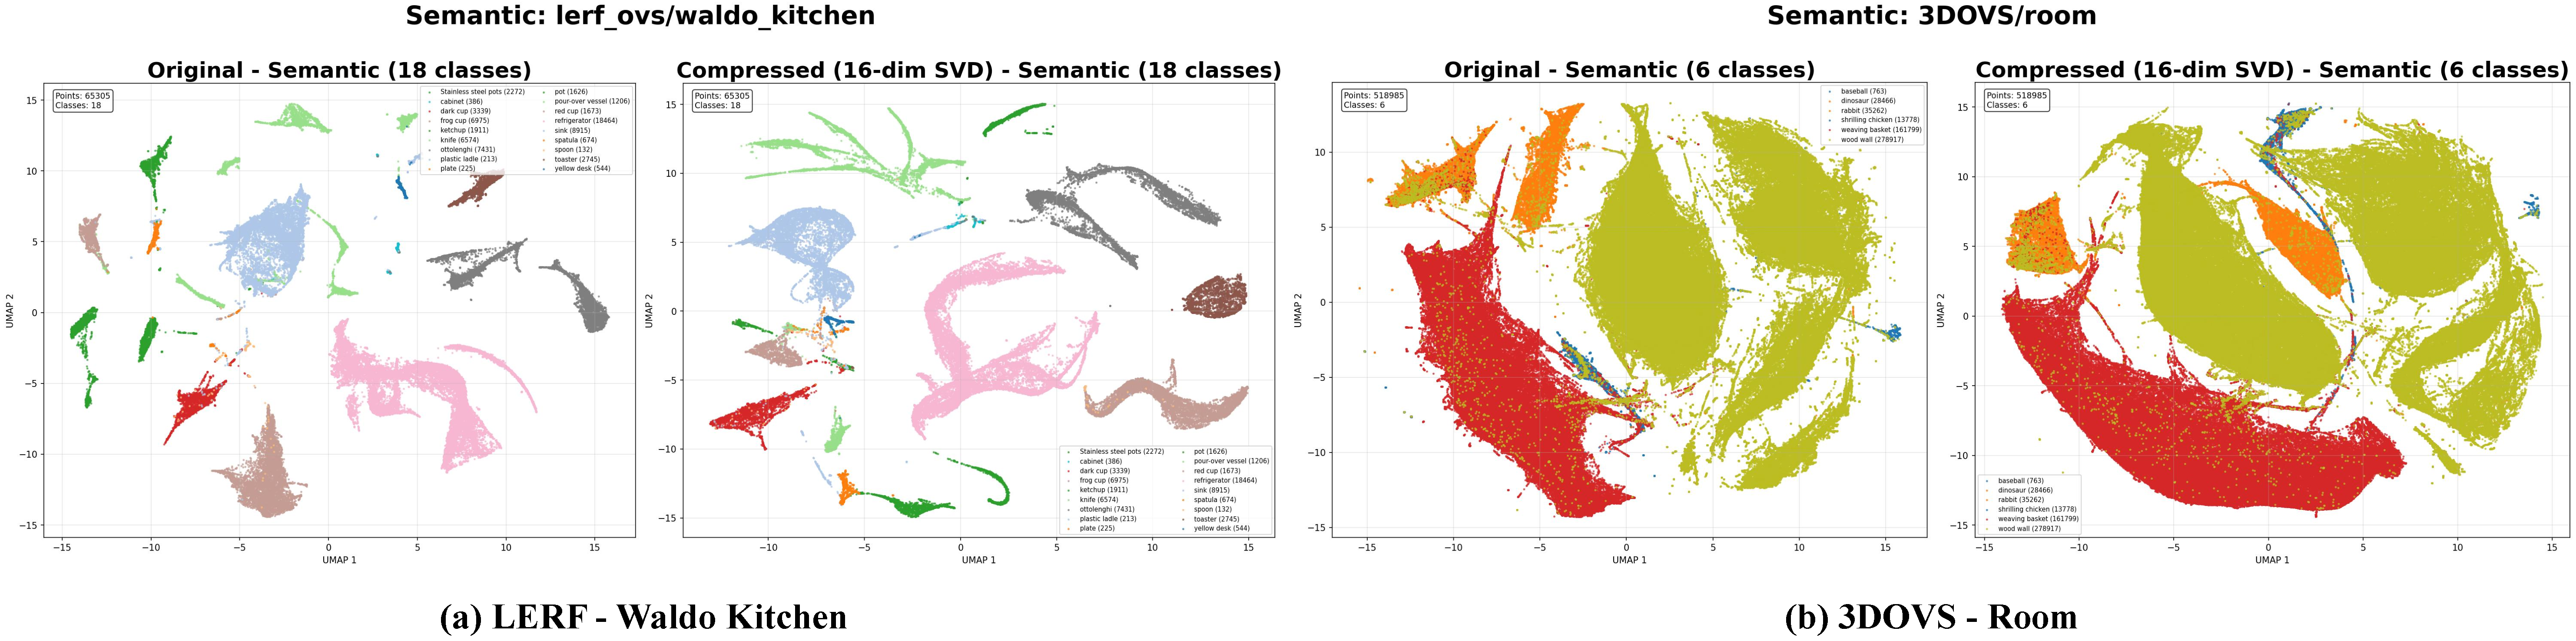
\includegraphics[width=\textwidth]{figs/JM-Visual.pdf}
  \caption{Visual comparison of feature distributions before and after dimensionality reduction in the feature space on the LERF and 3DOVS datasets.}
  \label{fig:JM-visual}
\end{figure}

\begin{table}[tb]
  \caption{Analysis of JM Distance. We present the JM distances computed under a Gaussian distribution assumption, as well as the JM distances obtained after aggregating the high‑dimensional distributions using arithmetic mean (AM) and geometric mean (GM). The compressed average JM distance actually shows an increasing trend.}
  \label{tab:jm-dist}
  \centering
  \resizebox{\textwidth}{!}{
  \begin{tabular}{@{}l|c|cccc|ccccc|c@{}}
    \toprule
    % 表头行：用 \multicolumn 覆盖竖线
    \multicolumn{1}{c}{\multirow{2}{*}{Setting}} & \multicolumn{1}{c}{\multirow{2}{*}{Metrics}} & \multicolumn{4}{c}{LERF} & \multicolumn{5}{c}{3D-OVS} & \multicolumn{1}{c}{\multirow{2}{*}{Avg}}\\
    \cmidrule(lr){3-6} \cmidrule(lr){7-11}
    \multicolumn{1}{c}{} & & Ramen & Figurines & Teatime & Kitchen & Bed & Bench & Room & Sofa & Lawn & \\
    \midrule
    & gaussian & 1.4128 & 1.4139 & 1.4110 & 1.4139 & 1.4142 & 1.4141 & 1.4142 & 1.4115 & 1.3875 & 1.4103\\
    origin & AM & 0.8061 & 0.9071 & 0.9522 & 0.9413 & 1.1786 & 1.0659 & 1.1303 & 1.1031 & 0.9342 & 1.0021\\
    & GM & 0.8506 & 0.9949 & 1.0322 & 1.0291 & 1.2492 & 1.1393 & 1.1987 & 1.1901 & 0.9702 & 1.0727\\
    \midrule
    & gaussian & 1.3887 & 1.4119 & 1.3994 & 1.4119 & 1.4142 & 1.4110 & 1.4137 & 1.4097 & 1.3013 & 1.3958($\textcolor{green}{-1.0\%}$)\\
    ours-16D & AM & 0.8992 & 1.0819 & 1.0661 & 1.1069 & 0.9475 & 1.0429 & 1.0045 & 1.0006 & 0.9539 & 1.0115($\textcolor{red}{+0.9\%}$)\\
    & GM & 0.9466 & 1.1829 & 1.1586 & 1.2319 & 1.1235 & 1.1397 & 1.1203 & 1.1649 & 0.9932 & 1.1179($\textcolor{red}{+4.2\%}$)\\
    \bottomrule
  \end{tabular}}
\end{table}

% 在这一节中，我们通过开放词汇场景领域常用的数据集，3DOVS与LERF数据集上的实验验证了SceneSplat-7k数据集中语言特征矩阵的低秩特性，并通过定量的方式验证了压缩后的特征空间的有效性。
In this section, we validate the low-rank property of the language feature matrix in the SceneSplat-7k \cite{li2025scenesplat} dataset through experiments on the commonly used open‑vocabulary scene datasets, namely 3DOVS \cite{liu2023weakly} and LERF\cite{lerf2023}, and quantitatively verify the effectiveness of the compressed feature space.

% 我们使用与SceneSplat相同的方法处理两个数据集，得到768维SigLIP2语言特征，并通过Occam's LGS聚合得到3D语言特征。随后，我们通过反投影的方式将2D标注映射到3DGS,并基于投票机制确定每个高斯的伪标签。我们使用UMap方法对原始特征空间和基于我们的方法压缩至16维的特征空间中各类别数据分布进行可视化，结果如图x所示。
% 压缩特征空间维度会细微影响各类别特征空间分布，但不影响类别间的可分性，原始高维空间中的不同簇在低维空间中亦不会重叠。
% Following the same procedure as in SceneSplat, we process both datasets to obtain 768‑dimensional SigLIP2 language features, which are then aggregated into 3D language features via Occam’s LGS \cite{cheng2024occamslgssimpleapproach}. The 2D annotations are subsequently back-projected onto the 3D Gaussians, and a voting mechanism is applied to assign pseudo‑labels to each Gaussian. We visualize the per‑class data distributions in the original feature space and in the 16‑dimensional feature space compressed by our method using UMAP, as shown in Figure \ref{fig:JM-visual}.
% While compressing the feature‑space dimension slightly alters the distribution of each class, it does not compromise inter‑class separability. The distinct clusters present in the original high‑dimensional space remain non‑overlapping after compression.
We follow SceneSplat’s procedure to process both datasets, extracting 768‑dim SigLIP2 \cite{tschannen2025siglip} language features and aggregating them into 3D language features via Occam’s LGS \cite{cheng2024occamslgssimpleapproach}. The 2D annotations are back‑projected onto 3D Gaussians, and a voting mechanism assigns pseudo‑labels to each Gaussian. In Figure \ref{fig:JM-visual}, we visualize the per‑class distributions in the original feature space and in our compressed 16‑dime space using UMAP.
Although feature‑space compression alters the within‑class distribution slightly, it preserves inter‑class separability: the distinct clusters observed in the original high‑dimensional space remain clearly separated after compression.

% 随后，我们使用JM距离对特征空间压缩前后各类别间的可分性进行定量分析。JM距离是一种衡量两个概率分布差异的距离度量，其值域为[0, √2]，值越大表示两类别的可分性越好。JM距离的定义基于巴氏距离，对于类别i,j，其概率分布$\tilde{p}_i(x)$与$\tilde{p}_j(x)}$间的巴氏距离为：
Subsequently, we employ the Jeffries-Matusita distance to quantitatively analyze the inter‑class separability before and after feature‑space compression. The JM distance, defined on the basis of the Bhattacharyya distance, measures the divergence between two probability distributions, ranging from 0 to $\sqrt{2}$, with larger values indicating better separability between two classes. The Bhattacharyya distance $B_{ij}$ between the probability distributions $\tilde{p}_i(x)$ and $\tilde{p}_j(x)$ is given by:
\begin{equation}
    B_{ij} = -\ln \left( \int \sqrt{\tilde{p}_i(x) \, \tilde{p}_j(x)} \, \mathrm{d}x \right)
\end{equation}
Hence, the JM distance between classes i and j is defined as $\text{JM}_{ij} = \sqrt{2(1 - e^{-B_{ij}})}$. We compute the average JM distance $\overline{\text{JM}}$ across all class pairs in a scene, where $c$ denotes the total number of classes.
\begin{equation}
    \overline{\text{JM}} = \frac{2}{c(c-1)} \sum_{i=1}^{c} \sum_{j>i}^{c} \sqrt{2(1 - e^{-B_{ij}})}
\end{equation}

% 实际计算过程中，需要先确定类别的分布以计算巴氏距离。当假设所有类别均为高斯分布时，类别i,j间的巴氏距离为：
To compute the Bhattacharyya distance in practice, the distribution of each class must first be estimated. Under the assumption that all classes follow Gaussian distributions, the Bhattacharyya distance between classes i and j is:
\begin{equation}
    B_{ij}^{\text{g}} = \frac{1}{8} (\mathbf{M}_i - \mathbf{M}_j)^T \left( \frac{\mathbf{V}_i + \mathbf{V}_j}{2} \right)^{-1} (\mathbf{M}_i - \mathbf{M}_j) + \frac{1}{2} \ln \left( \frac{ | \frac{\mathbf{V}_i + \mathbf{V}_j}{2} | }{ \sqrt{ | \mathbf{V}_i | \cdot | \mathbf{V}_j | } } \right)
\end{equation}
where $\mathbf{M}_i$ and $\mathbf{M}_j$ are the mean vectors of classes i and j, respectively, and $\mathbf{V}_i$ and $\mathbf{V}_j$ are their corresponding covariance matrices.
% 然而，所有类别不一定都满足高斯分布。同时，基于高斯分布假设计算JM距离时，高维特征的JM距离理论上大于低维特征，因为每个独立维度都为Bhattacharyya距离贡献非负值，产生累积的"维度红利"效应。因此，我们使用离散化方式计算任意分布间的JM距离。
% 具体而言，对每个维度的特征值进行离散化分箱统计得到各维度直方图，计算每维度的Bhattacharyya系数后通过算术/几何平均聚合，最后转换为JM距离。采用平均聚合的原因是各维度一般不满足相互独立，通过按维度平均的策略避免维度红利。基于算术和几何平均聚合的JM距离计算公式分别如Eq25,Eq26。
% However, not all classes necessarily follow Gaussian distributions. Moreover, when computing JM distances under the Gaussian assumption, the distance for high‑dimensional features is theoretically greater than that for low‑dimensional ones, because each independent dimension contributes a non‑negative value to the Bhattacharyya distance, resulting in a cumulative ``dimensional bonus'' effect. Therefore, we compute JM distances between arbitrary distributions using a discretization approach.
% Specifically, the feature values in each dimension are discretized into bins to obtain per‑dimensional histograms. The Bhattacharyya coefficient is computed for each dimension and then aggregated via arithmetic or geometric averaging, after which it is converted to  JM distance. Averaging across dimensions is adopted because the dimensions are generally not independent. This strategy avoids the dimensional bonus effect. 
Not all classes follow Gaussian distributions, and under the Gaussian assumption, high‑dimensional features obtain artificially inflated JM distances because each independent dimension adds a non‑negative contribution—a “dimensional‑bonus” effect. To avoid this, we compute JM distances via discretization. We bin the feature values in each dimension, compute the Bhattacharyya coefficient per dimension, aggregate the coefficients by arithmetic or geometric averaging, since dimensions are generally correlated, and finally convert the result to JM distance. This procedure makes no Gaussian or independence assumptions and eliminates the dimensional bonus.
The formulas for the JM distance based on arithmetic and geometric‑mean aggregation are given in Eq.\eqref{eq:jmam} and Eq.\eqref{eq:jmgm}, respectively.
\begin{equation}
    \text{JM}_{ij}^{\text{AM}} = \sqrt{2 \left(1 - \frac{1}{D} \sum_{d=1}^{D} \sum_{k=1}^{n_{b}} \sqrt{\tilde{p}_i(d,k) \cdot \tilde{p}_j(d,k)}\right)} 
    \label{eq:jmam}
\end{equation}
\vspace{-3.0em}
\begin{equation}
    \text{JM}_{ij}^{\text{GM}} = \sqrt{2 \left(1 - \exp\left(\frac{1}{D} \sum_{d=1}^{D} \ln\left(\sum_{k=1}^{n_{b}} \sqrt{\tilde{p}_i(d,k) \cdot \tilde{p}_j(d,k)}\right)\right)\right)}
    \label{eq:jmgm}
\end{equation}
where $n_b$ denotes the number of bins in the histogram, and $D$ indicates the feature dimensionality. 
% 各场景3种平均JM距离如表2所示。使用我们的方法压缩至16维的特征空间，其平均JM距离甚至整体高于原始特征空间，这证明了原始特征矩阵的冗余性。即使在高度压缩的低维空间中，不同类别特征分布间依然能保持良好的可分性，因此在不损失分类性能前提下进行降维是可能的。
The average JM distances across scenarios for different aggregation methods are presented in Table \ref{tab:jm-dist}. Our 16‑dimensionally compressed feature space yields an even higher average JM distance than the original space, confirming the redundancy of the original feature matrix. The distinct classes remain well‑separable in this low‑dimensional space, demonstrating that dimensionality reduction can be achieved without degrading classification performance.

\section{Experiments}
\label{sec:experiment}
% 
\begin{figure}[tb]
  \centering
  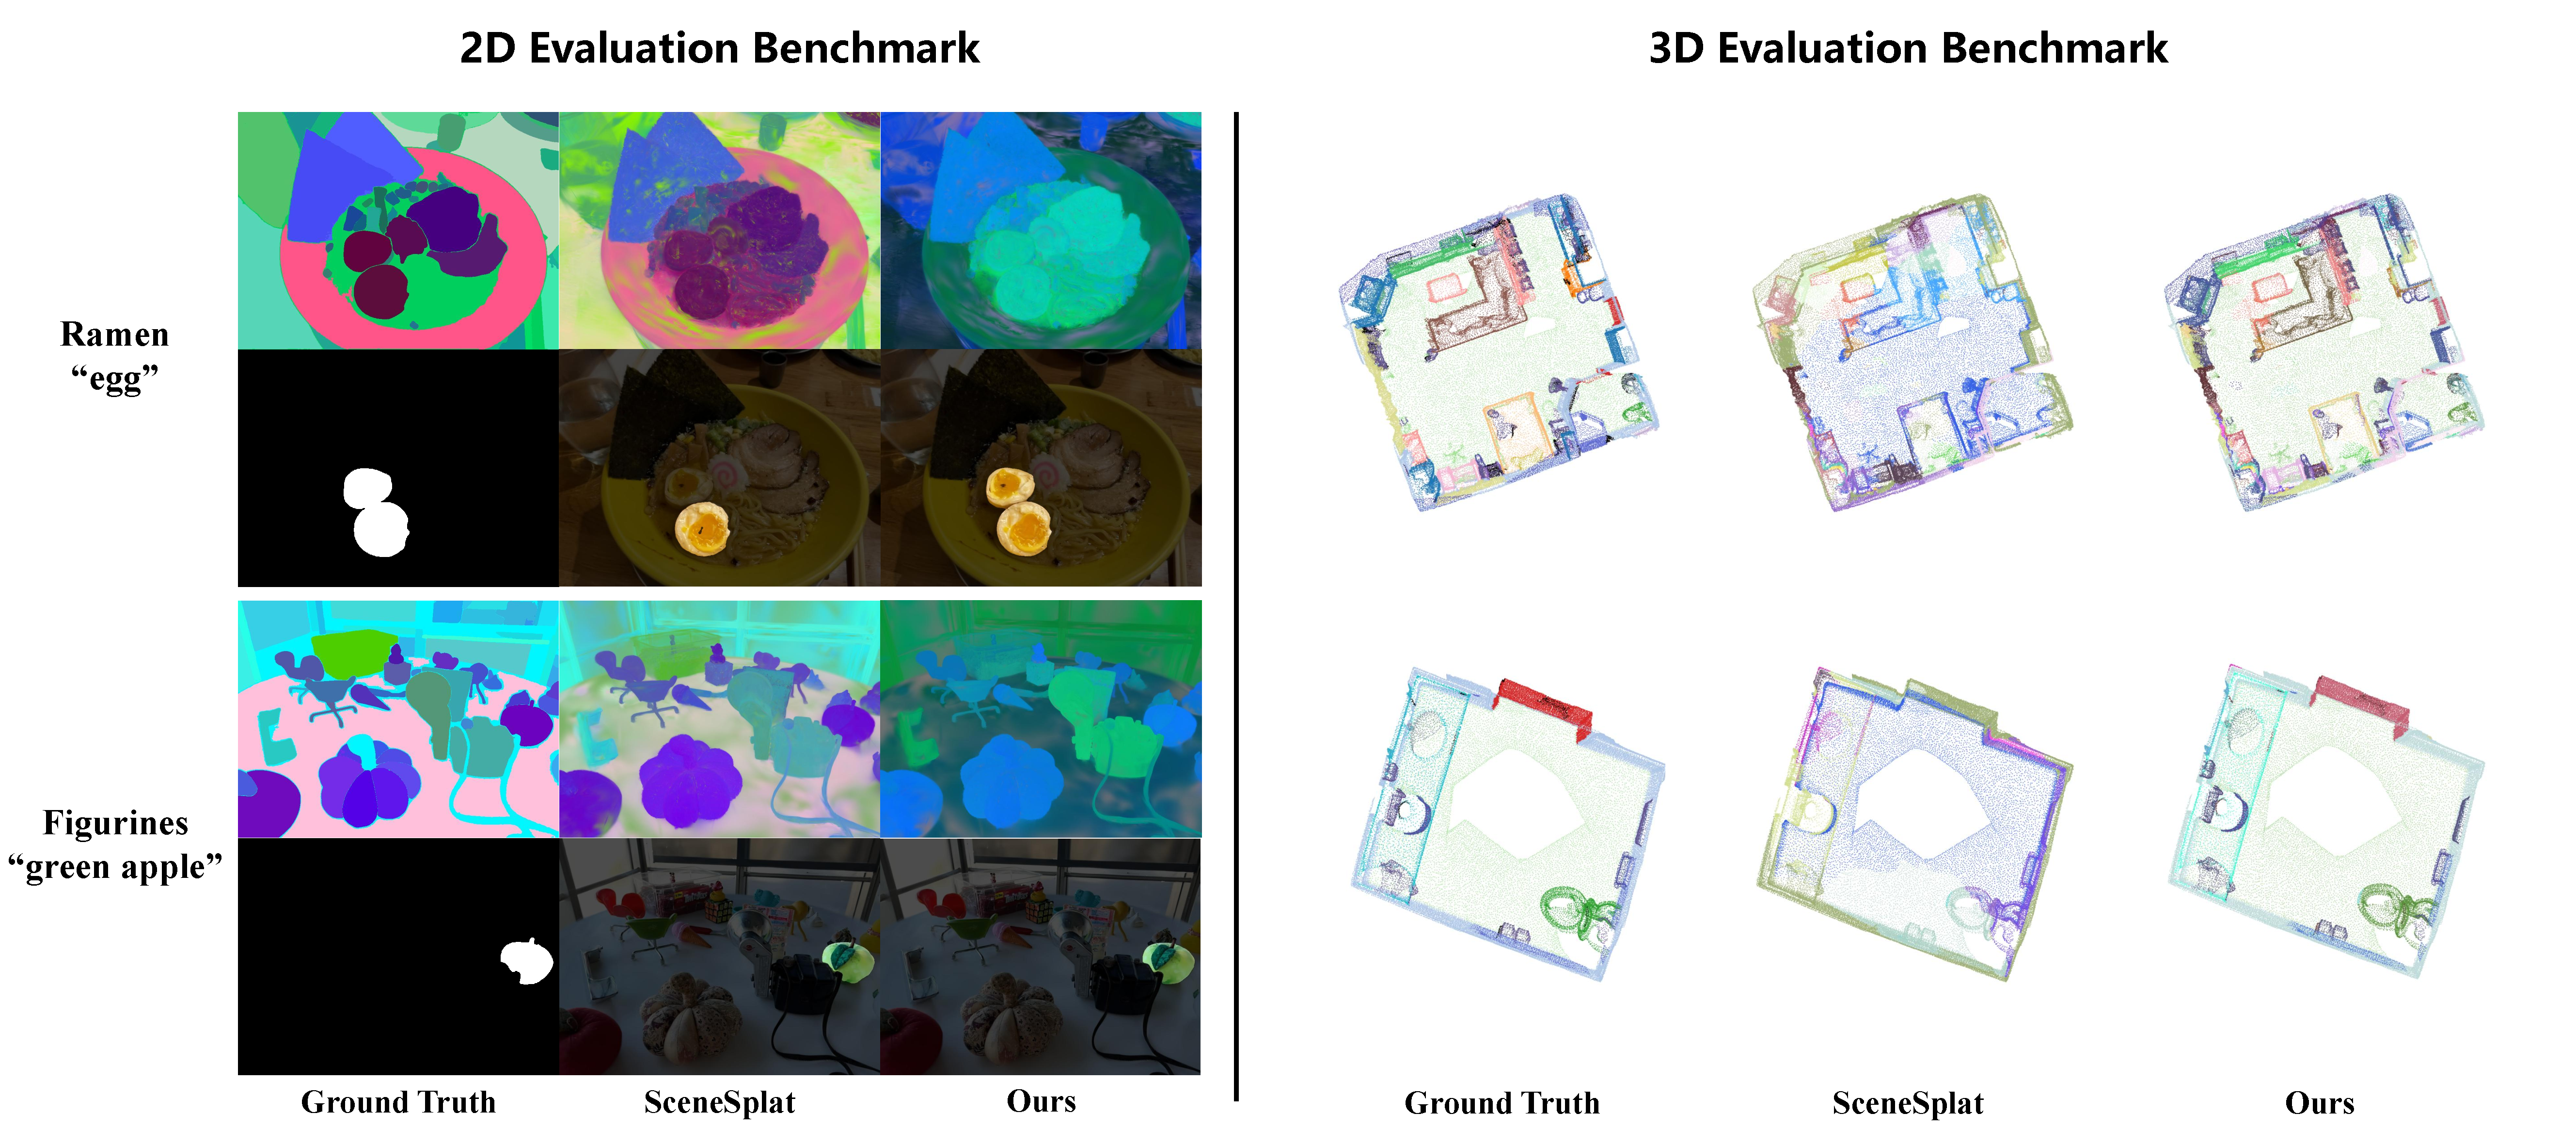
\includegraphics[width=\textwidth]{figs/Visualize-All.pdf}
  \caption{\textbf{Left:} PCA visualization of semantic features on the LERF dataset. \textbf{Right:} Qualitative results of zero‑shot 3D semantic segmentation on ScanNet++ scenes.}
  \label{fig:Visualize}
\end{figure}

\subsection{Setup}
\noindent\textbf{Datasets.}
% 我们遵循 SceneSplat 的评估协议，在涵盖 超300个语义类别 的 ScanNet（20 类与 200 类划分）、ScanNet++（100 类）以及 Matterport3D（160 类）三个数据集上进行训练与评估。该协议在三维空间中综合衡量几何一致性、语义准确性（如前景平均交并比 f‑mIoU 与前景平均准确率 f‑mAcc）以及计算效率。我们设置的查询物体涵盖从鼠标到床等多种尺度，以检验模型对不同规模物体的开放词汇理解能力。
We adopt SceneSplat’s evaluation protocol, training and testing on ScanNet (20/200 classes), ScanNet++ (100 classes), and Matterport3D (160 classes), together covering over 300 semantic categories. The protocol evaluates 3D geometric consistency, semantic accuracy (e.g., foreground mIoU and mAcc), and computational efficiency. Using 160 classes for Matterport3D follows SceneSplat’s fine‑grained setting to test recognition of long‑tail objects. 
% Our object queries span scales from a mouse to a bed, assessing open‑vocabulary understanding across sizes.
% 我们同样遵循LERF与3DOVS的评估协议，在2D渲染图上评估语义性能。
% LERF数据集包含多样物体的日常室内场景，我们根据LERF评估协议[13]，在常用场景Ramen、Figurines、Teatime和Waldo Kitchen上进行了定量评估。在这些场景中，我们评估了开放词汇分割任务（mIoU）与定位精度。
% 3D-OVS数据集涵盖多样背景下的长尾物体，我们在sofa、lawn、bed、room和bench五个场景中评估分割性能。评估时，我们采用[23]为这两个数据集提供的标注。
We also evaluate 2D semantic performance following LERF\cite{lerf2023} protocols. On LERF’s everyday indoor scenes, we report open‑vocabulary segmentation (mIoU) and localization accuracy on standard evaluation scenes.
% For the 3D‑OVS dataset, which includes long‑tail objects in varied backgrounds, we evaluate segmentation performance on five scenes: sofa, lawn, bed, room, and bench. 
% The annotations used for both datasets are those provided by \cite{qin2024langsplat}.
The annotations are provided by \cite{qin2024langsplat}.

\noindent\textbf{Baselines.}
% 在SceneSplat数据集上，我们与SceneSplat等[Mosaic3D，OV3D，RegionPLC，PLA，OpenScene]当前最先进的通用3D开放词汇分割方法进行比较。在LERF与3DOVS数据集上，我们与当前最先进的Per-Scene方法进行比较，同时也和SceneSplat比较。对于大多数方法，我们直接报告其已发表的最佳定量结果。
On the SceneSplat dataset, we compare with state-of-the-art general 3D open-vocabulary segmentation methods such as SceneSplat \cite{li2025scenesplat,lee2025mosaic3d,jiang2024open,yang2024regionplc,ding2022language,peng2023openscene}. On the LERF and 3D-OVS datasets, we compare with state-of-the-art Per-Scene methods\cite{drsplat25,cheng2024occamslgssimpleapproach}, and also with SceneSplat. For most methods, we directly report their best published quantitative results.

\noindent\textbf{Implementations.} The implementation details are provided in the supplement.

\subsection{Comparison}
\begin{table}[tb]
\caption{Zero-Shot 3D Semantic Segmentation on the Fine-Grained ScanNet++ (100 classes), Matterport3D (160 classes) and ScanNet200 (200 classes) Benchmarks.}
  \label{tab:scene-splat}
  \centering
  \resizebox{\textwidth}{!}{
\begin{tabular}{l|l|c|cc|cc|cc}
\toprule
 \multirow{2}{*}{Method} & \multirow{2}{*}{Training Source} & Model & \multicolumn{2}{c|}{ScanNet200} & \multicolumn{2}{c|}{Matterport3D} & \multicolumn{2}{c}{ScanNet++} \\
 & & Params & f-mIoU & f-mAcc & f-mIoU & f-mAcc & f-mIoU & f-mAcc \\
 \midrule
 OpenScene\cite{peng2023openscene} & SN & 14.69M & 6.4 & 12.2 & 5.7 & 10.7 & 8.8 & 14.7 \\
 PLA\cite{ding2022language} & SN & \underline{11.73M} & 1.8 & 3.1 & - & - & - & - \\
 RegionPLC\cite{yang2024regionplc} & SN & 46.72M & 9.2 & 16.4 & 6.2 & 13.3 & 11.3 & 20.1 \\
 OV3D\cite{jiang2024open} & SN & - & 8.7 & - & - & - & - & - \\
 Mosaic3D\cite{lee2025mosaic3d} & SN & 683.72M & 13.0 & 24.5 & 8.6 & 17.8 & \textbf{16.2} & \textbf{27.1} \\
 SceneSplat\cite{li2025scenesplat} & SN & 91.72M & \underline{18.9} & \underline{31.7} & \textbf{10.8} & \textbf{18.7} & \underline{14.7} & 24.7 \\
 Ours & SN & \textbf{9.58M} & \textbf{19.0} & \textbf{31.9} & \underline{10.6} & \underline{18.3} & \underline{14.7} & \underline{24.9} \\
 % Ours(PTv3) & SN & -M & - & - & - & - & - & - \\
 \midrule
 Mosaic3D & SN, SN++, ARKitS, MP3D, S3D & 683.72M & 15.7 & 28.3 & \underline{13.1} & 27.7 & 18.0 & 29.0 \\
 SceneSplat & SN++ & 91.72M & 11.8 & 19.2 & 10.6 & 18.6 & 26.8 & 45.3 \\
 SceneSplat & SN, SN++, MP3D & 91.72M & \textbf{21.4} & \textbf{38.7} & \textbf{13.8} & \underline{31.8} & \textbf{28.4} & \textbf{50.0} \\
 Ours & SN, SN++, MP3D & \textbf{9.58M} & \underline{21.2} & \underline{38.6} & \textbf{13.8} & \textbf{31.9} & \underline{28.0} & \underline{49.6} \\
 % Ours(PTv3) & SN, SN++, MP3D & -M & - & - & - & - & - & - \\
\bottomrule
\end{tabular}}
\end{table}


\begin{table*}[tb]
\centering
\caption{Performance of open vocabulary 3D object selection and rendering on LERF. Accuracy is measured by mAcc@0.25. $*$ indicates officially provided pre‑trained weights. }
\label{tab:lerf-ovs}
% We observe that the SceneSplat checkpoint suffers from severe mode collapse, resulting in only foreground‑background separation in LERF.
% \setlength{\tabcolsep}{3.5mm}
\resizebox{\textwidth}{!}{
\begin{tabular}{@{}l|cccccccc|cc|c}
\toprule
\multirow{2}{*}{Methods} &
\multicolumn{2}{c} {figurines} & 
\multicolumn{2}{c} {ramen} & 
\multicolumn{2}{c} {teatime} & 
\multicolumn{2}{c|} {waldo-kitchen} & 
\multicolumn{2}{c|} {Average} & \multirow{2}{*}{Time}\\ 
& mIou$\uparrow$ & mAcc$\uparrow$ & mIou$\uparrow$ & mAcc$\uparrow$ & mIou$\uparrow$ & mAcc$\uparrow$ & mIou$\uparrow$ & mAcc$\uparrow$ & mIou$\uparrow$ & mAcc$\uparrow$ \\
\midrule 
% \specialrule{0.4pt}{0pt}{0pt}
LangSplat\cite{qin2024langsplat} & 10.16 & 8.93 & 7.92 & 11.27 & 11.38 & 20.34 & 9.18 & 9.09 & 9.66 & 12.41 & >1h\\
LEGaussians\cite{shi2024language} & 17.99 & 23.21 & 15.79 & 26.76 & 19.27 & 27.12 & 11.78 & 18.18 & 16.21 & 23.82 & >4h\\
GSGrouping\cite{ye2024gaussian} & 55.38 & 76.61 & 32.58 & 54.45 & 33.82 & 52.21 & 30.02 & 50.23 & 37.95 & 58.38 & >2h\\
OpenGaussian\cite{wu2024opengaussian} & 39.29 & 55.36 & 31.01 & 42.25 & 60.44 & 76.27 & 22.70 & 31.82 & 38.36 & 51.43 & >1h\\
InstanceGS\cite{li2025instancegaussian} & 52.04 & 69.64 & 22.36 & 38.03 & 53.35 & 71.19 & 37.07 & 54.55 & 41.21 & 58.35 & >2h\\
Dr.Splat\cite{drsplat25} & 54.42 & 80.36 & 24.33 & 35.21 & 57.35 & 77.97 & 37.05 & 63.64 & 43.29 & \underline{64.30} & 0.57min\\
% CAGS & 60.85 & 82.14 & 36.29 & 46.48 & 68.40 & 86.44 & 37.62 & 63.64 & 50.79 & 69.62 \\
% SLAG & 48.10 & 69.95 & 24.76 & 64.77 & 56.12 & 81.68 & 27.55 & 48.88 & 39.13 & 66.32 \\
LUDVIG\cite{marrie2025ludvig} & 54.43 & - & 50.11 & - & 69.01 & - & 56.03 & - & \textbf{57.40} & - & 10min\\
OccamLGS\cite{cheng2024occamslgssimpleapproach} & 56.12 & 75.00 & 42.26 & 45.07 & 68.66 & 79.66 & 55.92 & 81.82 & \underline{55.74} & \textbf{70.39} & 2min \\
\midrule
% \specialrule{0.4pt}{0pt}{0pt}
SceneSplat* & 45.58 & 67.86 & 26.75 & 38.03 & 49.02 & 62.71 & 38.75 & 50.00 & 40.03 & 54.65 & \underline{0.18min} \\
Ours & 41.87 & 60.71 & 39.22 & 42.25 & 67.83 & 81.36 & 47.74 & 68.18 & 49.17 & 63.13 & \textbf{0.04min}\\
\bottomrule
\end{tabular}}
\end{table*}

% 表4展示了在细粒度数据集ScanNet++（100类）、Matterport3D（160类）和ScanNet200（200类）上的零样本3D语义分割结果。我们使用压缩后的数据集训练PTv3的轻量化变体，关于网络架构的消融将在附录中展示。
% 当仅在ScanNet上训练时，我们的方法在ScanNet200上达到了最优，同时在另两个数据集上达到了与SceneSplat相近的性能。
% 在扩展训练数据后，我们的方法在Matterport3D数据集上取得了领先，而在其他数据集上同样取得了与SceneSplat接近的性能。值得注意的是，我们的方法使用了最轻量化的模型，相比SceneSplat小将近10倍，其中一大原因是我们大幅压缩了特征维度，使decoder的参数量大大减小。
Table \ref{tab:scene-splat} presents the zero-shot 3D semantic segmentation results on the fine-grained datasets ScanNet++, Matterport3D, and ScanNet200. We train a lightweight variant of PTv3\cite{wu2024ptv3,yuelitept2026} using the compressed dataset, and ablations on the network architecture are provided in the appendix.
Trained solely on ScanNet, our method achieves the best performance on ScanNet200 and matches SceneSplat on the other two datasets. With expanded training data, it leads on Matterport3D and remains competitive elsewhere. Critically, our model is nearly 10× smaller than SceneSplat, largely due to feature dimensionality compression that drastically reduces decoder parameters.

% 表5展示了我们的方法在LERF数据集上的open vocabulary 3D object selection性能。SceneSplat和我们的方法主要由3D特征监督，在2D分割指标上相比其他直接基于2D语义监督的方法稍有劣势，但是我们的方法实现了最快的推理速度，实现了准实时的开放词汇语义推理。
Table \ref{tab:lerf-ovs} presents the open‑vocabulary 3D object selection performance of our method on the LERF dataset. Both SceneSplat and our method are primarily supervised by 3D features, resulting in slightly lower 2D segmentation metrics compared to other methods that rely directly on 2D semantic supervision. However, our method achieves the fastest inference speed, enabling near real‑time open‑vocabulary semantic inference.

% 如图4所示，我们的方法在2D和3D开放词汇分割评估体系下均实现了与SceneSplat接近的性能，实现了准确的开放词汇分割与物体查询。值得注意的是，我们的特征图可视化与SceneSplat和GT略有区别，这是因为我们已经将特征投影到低维空间，此时通过PCA进行可视化会与直接对原始特征PCA存在差异。然而，可以直观感受到，即使在低维空间中，不同物体间特征依旧保持良好的可分性，这印证了第4章的分析。此外，得益于SVD分解的线性特性，我们能够通过简单的线性投影将原始特征与压缩后的特征在低维空间中重新对齐，从而在低维空间直接进行查询，详细的步骤将在附录中展示。每场景特征对齐的用时均在毫秒级别，相比基于Auto encoder的特征降维方法，我们能节省大量per scene优化成本。
As shown in Fig. \ref{fig:Visualize}, our method delivers accurate open‑vocabulary segmentation and object querying, achieving performance close to SceneSplat in both 2D and 3D evaluations. While our feature‑map visualizations differ slightly from SceneSplat and the ground truth—because we project features into a low‑dimensional space where PCA behaves differently—different objects remain clearly separable, confirming the analysis in Section \ref{sec:analysis}. Moreover, the linearity of SVD allows original and compressed features to be realigned via a simple projection, enabling direct low‑dimensional querying (details in appendix). This per‑scene alignment takes only milliseconds, avoiding the costly per‑scene optimization required by Auto‑Encoder‑based reduction.

\subsection{Ablation Study}
% 表6展示了我们在Scannet200和LERF数据集上的消融，我们提出的方法相比仅使用SVD压缩特征均有显著提升，这是因为RPCA对特征维度的噪声具有鲁棒性，Density-Invariant learning对空间维度的噪声具有鲁棒性。
Ablation on ScanNet200 and LERF (Table \ref{tab:ablation-m}) shows our full method surpasses SVD‑only compression. The gain comes from RPCA’s robustness to feature noise and Density‑Invariant Learning’s robustness to spatial noise.
% 表7展示了对压缩特征维度的消融，当使用32维度的特征时达到了接近SOTA的水平，而16维特征则在精度与推理效率间取得了平衡。
Table \ref{tab:ablation_rank_tradeoff} ablates compressed feature dimensions. 32‑D features achieve near‑SOTA accuracy, whereas 16‑D features balance accuracy and inference efficiency.
% 表8展示了我们的Structured RPCA算法在效率上相比普通RPCA快了3个数量级，误差尽管增大却在可接受范围内，其原因是对原始矩阵中相似行的近似。
Table \ref{tab:ablation_latency} shows that our Structured RPCA is three orders of magnitude faster than standard RPCA. The slight increase in error remains acceptable, resulting from our approximation of similar matrix rows.
\vspace{-1.0em}
\begin{table}[htbp]
    \centering
    % 第一个表格
    \begin{minipage}[t]{0.5\textwidth}
    \caption{Ablation study on different components of our method on ScanNet200 and LERF datasets using 16-dim features.}
    \label{tab:ablation-m}
    \centering
    \resizebox{1\linewidth}{!}{
      \begin{tabular}{@{}lcccc@{}}
        \toprule
        \multirow{2}{*}{Method} & \multicolumn{2}{c}{ScanNet200} & \multicolumn{2}{c}{LERF} \\
        \cmidrule(lr){2-3} \cmidrule(lr){4-5}
        & mIoU & mAcc & mIoU & mAcc \\
        \midrule
        Full Method (Ours) & 19.0 & 31.9 & 49.2 & 63.1 \\
        w/o Density-Invariant & 18.4 & 31.2 & 44.1 & 60.9 \\
        w/o RPCA & 18.7 & 31.5 & 46.2 & 61.3 \\
        Only SVD & 18.2 & 30.8 & 41.3 & 59.2 \\
        \bottomrule
      \end{tabular}
    }
    \end{minipage}%
    \hfill%
    % 第二个表格
    \begin{minipage}[t]{0.48\textwidth}%
    \caption{Accuracy-latency trade-off with varying feature dimensions on LERF.}
    \vspace{-1.0em}
    \label{tab:ablation_rank_tradeoff}
    \centering
    \resizebox{!}{1cm}{
    \begin{tabular}{@{}l|cc|cc@{}}
    \toprule
    Rank & mIoU & mAcc & Latency (s) & Speedup \\
    \midrule
    768  & - & - & 10.98 & 1.00$\times$ \\
    32   & 55.82 & 67.52 & 3.39 & 2.95$\times$ \\
    16   & 49.17 & 63.13 & 2.44 & 4.50$\times$ \\
    8    & 43.64 & 57.15 & 2.15 & 4.65$\times$ \\
    \bottomrule
    \end{tabular}}

    \caption{RPCA ablations on LERF.}
    \vspace{-1.0em}
    \label{tab:ablation_latency}
    \centering
    \resizebox{!}{1cm}{
    \begin{tabular}{@{}l|cc@{}}
    \toprule
    Method & Error & Latency \\
    \midrule
    RPCA-CPU & $6.28 \times 10^{-6}$ & >2h \\
    RPCA-GPU & $6.28 \times 10^{-6}$ & 330.55s \\ 
    Structured RPCA & $9.37 \times 10^{-3}$ & 0.18s \\ %0.1782
    \bottomrule
    \end{tabular}}
    \end{minipage}
\end{table}
\vspace{-3.0em}
\section{Conclusion}
In this paper, we tackle the storage and computational inefficiency in open‑vocabulary 3D Gaussian Splatting. We propose a two‑stage compression pipeline, Grid‑based Feature Approximation and Structured RPCA, that jointly exploits redundancy in 3D language features, preserving semantic separability in a compact feature space. Coupled with Grid‑Guided Density‑Invariant Learning for input‑density robustness, our approach compresses SceneSplat‑7k language features by $\sim100\times$. The resulting lightweight model achieves state‑of‑the‑art accuracy with significantly lower latency, enabling efficient and real‑time 3D scene understanding.

\iffalse
\section{Introduction}
\label{sec:intro}

This document serves as an example submission to ECCV \ECCVyear{}.
It illustrates the format authors must follow when submitting a paper. 
At the same time, it gives details on various aspects of paper submission, including preservation of anonymity and how to deal with dual submissions.
We advise authors to read this document carefully.

The document is based on Springer LNCS instructions as well as on ECCV policies, as established over the years.

\section{Initial Submission}

\subsection{Language}
All manuscripts must be in English.


\subsection{Template}
Papers must be prepared with the official LNCS style from Springer.
This applies to both review and camera-ready versions.
Springer requires manuscripts to be prepared in \LaTeX{} (strongly encouraged) or Microsoft Word. 

Authors preparing their paper with \LaTeX{} must use the template provided by ECCV, which is based on the corresponding Springer class file \texttt{llncs.cls} but includes line numbers for review (\cref{sec:line-numbering}) and properly anonymizes the paper for review (as in this example document).
Authors who -- for whatever reason -- cannot use \LaTeX{} can alternatively use the official LNCS Word template from Springer.
However, it is the authors' responsibility to ensure that the resulting PDF file is consistent with this example paper and follows it as closely as possible (\ie, includes line numbers, is properly anonymized, \etc).

We would like to stress that the class/style files and the template must not be manipulated and that the guidelines regarding font sizes and format must be adhered to. 
For example, please refrain from using any \LaTeX{} or \TeX{} command that modifies the layout settings of the template (\eg, \verb+\textheight+, \verb+\vspace+, \verb+\baselinestretch+, \etc).
Such manual layout adjustments should be limited to very exceptional cases.
This is to ensure that the end product is as homogeneous as possible.

Papers that differ significantly from the required style may be rejected without review.


\subsubsection{Fonts.}
Springer's templates for \LaTeX{} are based on CMR, and the XML templates for Word are based on Times. 
We ask you to use the font according to the template used for your papers. 
Specifically, please refrain from using Times when preparing your paper with \LaTeX{}.
Using a different font can be interpreted as purposely circumventing the length limitations and may lead to rejection without review.


\subsection{Paper Length}
Papers submitted for review must be complete. 
The length should match that intended for final publication. 
Papers accepted for the conference will be allocated 14 pages (plus additional pages for references) in the proceedings. 
Note that the allocated 14 pages do not include the references. 
The reason for this policy is that we do not want authors to omit references for sake of space limitations.

Papers with more than 14 pages (excluding references) will be rejected without review.
This includes papers where the margins and formatting including the font are deemed to have been significantly altered from those laid down by this style guide.

The reason such papers will not be reviewed is that there is no provision for supervised revisions of manuscripts. 
The reviewing process cannot determine the suitability of the paper for presentation in 14 pages if it is reviewed in 16.


\subsection{Paper ID}
It is imperative that the paper ID is mentioned on each page of the manuscript of the review version.
Enter your paper ID in the appropriate place in the \LaTeX{} template (see \texttt{\%TODO REVIEW}).
The paper ID is a number automatically assigned to your submission when registering your paper submission on the submission site.


\subsection{Line Numbering}
\label{sec:line-numbering}
All lines should be numbered in the initial submission, as in this example document. 
This makes reviewing more efficient, because reviewers can refer to a line on a page. 
Line numbering is removed in the camera-ready version.


\section{Policies}
The policies governing the review process of ECCV \ECCVyear{} are detailed on the conference webpage (see \url{ https://eccv.ecva.net/Conferences/2026/SubmissionPolicies}), such as regarding confidentiality, dual submissions, double-blind reviewing, plagiarism, and more. 
By submitting a paper to ECCV, the authors acknowledge that they have read the submission policies and that the submission follows the rules set forth.

Accepted papers will be published in LNCS proceedings with Springer.
To that end, authors must follow the Springer Nature Code of Conduct for Authors (see \url{https://www.springernature.com/gp/authors/book-authors-code-of-conduct}).
We would like to draw particular attention to the policies regarding figures and illustrations, as well as ethical approval and informed consent, which are also reproduced on the ECCV website.


\section{Preserving Anonymity}
\label{sec:blind}
ECCV reviewing is double blind, in that authors do not know the names of the area chair/reviewers of their papers, and the area chairs/reviewers cannot, beyond reasonable doubt, infer the names of the authors from the submission and the additional material. 
You must not identify the authors nor provide links to websites that identify the authors, neither in the paper nor in the supplemental material.
If you need to cite a different paper of yours that is being submitted concurrently to ECCV, you should \emph{(1)} cite these papers anonymously, \emph{(2)} argue in the body of your paper why your ECCV paper is non-trivially different from these concurrent submissions, and \emph{(3)} include anonymized versions of those papers in the supplemental material.
Violation of any of these guidelines may lead to rejection without review. 

Many authors misunderstand the concept of anonymizing for blind review.
Blind review does not mean that one must remove citations to one's own work---in fact it is often impossible to review a paper unless the previous citations are known and available.

Blind review means that you do not use the words ``my'' or ``our'' when citing previous work.
That is all.
(But see below for tech reports.)

Saying ``this builds on the work of Lucy Smith [1]'' does not say that you are Lucy Smith;
it says that you are building on her work.
If you are Smith and Jones, do not say ``as we show in [7]'', say ``as Smith and Jones show in [7]'' and at the end of the paper, include reference 7 as you would any other cited work.

An example of a bad paper just asking to be rejected:
\begin{quote}
  \begin{center}
      An analysis of the frobnicatable foo filter.
  \end{center}

   In this paper we present a performance analysis of our previous paper [1], and show it to be inferior to all previously known methods.
   Why the previous paper was accepted without this analysis is beyond me.

   [1] Removed for blind review
\end{quote}

An example of an acceptable paper:
\begin{quote}
  \begin{center}
     An analysis of the frobnicatable foo filter.
  \end{center}

   In this paper we present a performance analysis of the  paper of Smith \etal [1], and show it to be inferior to all previously known methods.
   Why the previous paper was accepted without this analysis is beyond me.

   [1] Smith, L and Jones, C. ``The frobnicatable foo filter, a fundamental contribution to human knowledge''. Nature 381(12), 1-213.
\end{quote}

If you are making a submission to another conference at the same time, which covers similar or overlapping material, you may need to refer to that submission in order to explain the differences, just as you would if you had previously published related work.
In such cases, include the anonymized parallel submission [1] as supplemental material and cite it as
\begin{quote}
  [1] Authors. ``The frobnicatable foo filter'', ECCV \ECCVyear Submission ID 00324, Supplied as supplemental material {\tt 00324.pdf}.
\end{quote}

Finally, you may feel you need to tell the reader that more details can be found elsewhere, and refer them to a technical report.
For conference submissions, the paper must stand on its own, and not \emph{require} the reviewer to go to a tech report for further details.
Thus, you may say in the body of the paper ``further details may be found in~\cite{Anonymous24b}''.
Then submit the tech report as supplemental material.
Again, you may not assume the reviewers will read this material.

Sometimes your paper is about a problem, which you tested using a tool that is widely known to be restricted to a single institution.
For example, let's say it's 1969, you have solved a key problem on the Apollo lander, and you believe that the ECCV audience would like to hear about your
solution.
The work is a development of your celebrated 1968 paper entitled ``Zero-g frobnication: How being the only people in the world with access to the Apollo lander source code makes us a wow at parties'', by Zeus \etal.

You can handle this paper like any other.
Do not write ``We show how to improve our previous work [Anonymous, 1968].
This time we tested the algorithm on a lunar lander [name of lander removed for blind review]''.
That would be silly, and would immediately identify the authors.
Instead write the following:
\begin{quotation}
   We describe a system for zero-g frobnication.
   This system is new because it handles the following cases:
   A, B.  Previous systems [Zeus et al. 1968] did not  handle case B properly.
   Ours handles it by including a foo term in the bar integral.

   ...

   The proposed system was integrated with the Apollo lunar lander, and went all the way to the moon, don't you know.
   It displayed the following behaviours, which show how well we solved cases A and B: ...
\end{quotation}
As you can see, the above text follows standard scientific convention, reads better than the first version, and does not explicitly name you as the authors.
A reviewer might think it likely that the new paper was written by Zeus \etal, but cannot make any decision based on that guess.
He or she would have to be sure that no other authors could have been contracted to solve problem B.

For sake of anonymity, authors must omit acknowledgements in the review copy. 
They can be added later when you prepare the final copy.


\section{Formatting Guidelines}

\subsection{Headings}
Headings should be capitalized (\ie, nouns, verbs, and all other words except articles, prepositions, and conjunctions should be set with an initial capital) and should, with the exception of the title, be aligned to the left.
Only the first two levels of section headings should be numbered, as shown in \cref{tab:headings}.
The respective font sizes are also given in \cref{tab:headings}. 
Kindly refrain from using ``0'' when numbering your section headings.
Words joined by a hyphen are subject to a special rule. 
If the first word can stand alone, the second word should be capitalized.

\begin{table}[tb]
  \caption{Font sizes of headings. 
    Table captions should always be positioned \emph{above} the tables.
  }
  \label{tab:headings}
  \centering
  \begin{tabular}{@{}lll@{}}
    \toprule
    Heading level & Example & Font size and style\\
    \midrule
    Title (centered)  & {\Large\bf Lecture Notes \dots} & 14 point, bold\\
    1st-level heading & {\large\bf 1 Introduction} & 12 point, bold\\
    2nd-level heading & {\bf 2.1 Printing Area} & 10 point, bold\\
    3rd-level heading & {\bf Headings.} Text follows \dots & 10 point, bold\\
    4th-level heading & {\it Remark.} Text follows \dots & 10 point, italic\\
  \bottomrule
  \end{tabular}
\end{table}

Here are some examples of headings: 
``Criteria to Disprove Context-Freeness of Collage Languages'', ``On Correcting the Intrusion of Tracing Non-deterministic Programs by Software'', ``A User-Friendly and Extendable Data Distribution System'', ``Multi-flip Networks: Parallelizing GenSAT'', ``Self-determinations of Man''.


\subsection{Figures}
\label{sect:figures}
For \LaTeX{} users, we recommend integrating figures in your paper using the package \texttt{graphicx}.

It is essential that all illustrations are clear and legible. 
Vector graphics (rather than rasterized images) should be used for diagrams and schemas whenever possible. 
Please check that the lines in line drawings are not interrupted and have a constant width. 
Line drawings are to have a resolution of at least 800 dpi (preferably 1200 dpi).
Grids and details within figures must be clearly legible and may not be written one on top of the other. 
The lettering in figures should not use font sizes smaller than 6\:pt ($\sim$2\:mm character height). 

Figures should be numbered and should have a caption, which should always be positioned \emph{under} the figures, in contrast to the caption belonging to a table, which should always appear \emph{above} the table.
Figures and Tables should be cross-referred in the text.

If they are short, they are centered between the margins (\cf \cref{fig:short}). 
Longer captions, covering more than one line, are justified (\cref{fig:example} shows an example). 
Captions that do not constitute a full sentence, do not have a period.


\begin{figure}[tb]
  \centering
  \includegraphics[height=6.5cm]{eijkel2}
  \caption{One kernel at $x_s$ (\emph{dotted kernel}) or two kernels at $x_i$ and $x_j$ (\emph{left and right}) lead to the same summed estimate at $x_s$.
    This shows a figure consisting of different types of lines.
    Elements of the figure described in the caption should be set in italics, in parentheses, as shown in this sample caption. 
    The last sentence of a figure caption should generally end with a full stop, except when the caption is not a full sentence.
  }
  \label{fig:example}
\end{figure}

\begin{figure}[tb]
  \centering
  \begin{subfigure}{0.68\linewidth}
    \fbox{\rule{0pt}{0.5in} \rule{.9\linewidth}{0pt}}
    \caption{An example of a subfigure}
    \label{fig:short-a}
  \end{subfigure}
  \hfill
  \begin{subfigure}{0.28\linewidth}
    \fbox{\rule{0pt}{0.5in} \rule{.9\linewidth}{0pt}}
    \caption{Another example of a subfigure}
    \label{fig:short-b}
  \end{subfigure}
  \caption{Centered, short example caption}
  \label{fig:short}
\end{figure}

If possible (\eg, if you use \LaTeX) please define figures as floating objects. 
\LaTeX{} users, please avoid using the location parameter ``h'' for ``here''. 
If you have to insert a pagebreak before a figure, please ensure that the previous page is completely filled.


\subsection{Formulas}
Displayed equations or formulas are centered and set on a separate line (with an extra line or half line space above and below). 
Equations should be numbered for reference. 
The numbers should be consecutive within the contribution, with numbers enclosed in parentheses and set on the right margin.
For example,
\begin{align}
  \psi (u) & = \int_{0}^{T} \left[\frac{1}{2}
  \left(\Lambda_{0}^{-1} u,u\right) + N^{\ast} (-u)\right] \text{d}t \; \\
& = 0
\end{align}
and 
\begin{equation}
  E = m\cdot c^2.
  \label{eq:important}
\end{equation}
Please do not include section counters in the numbering.

Numbering equations makes reviewing more efficient, because reviewers can refer to a line on a page.  
It is important for readers to be able to refer to any particular equation.
Just because you did not refer to it in the text does not mean some future reader might not need to refer to it.
It is cumbersome to have to use circumlocutions like ``the equation second from the top of page 3''.
(Note that the ruler will not be present in the final copy, so is not an alternative to equation numbers).
All authors will benefit from reading Mermin's description of how to write mathematics:
\url{https://doi.org/10.1063/1.2811173}.

% No color equations in Springer publications.
Equations should never be in color and should be punctuated in the same way as ordinary text.
They should not be pasted in as figures.


\subsubsection{Lemmas, Propositions, and Theorems.}
The numbers accorded to lemmas, propositions, and theorems, \etc should appear in consecutive order, starting with Lemma 1. 
Please do not include section counters in the numbering like ``Theorem 1.1''.


\subsection{Footnotes.}
The superscript numeral used to refer to a footnote appears in the text either directly after the word to be discussed or -- in relation to a phrase or a sentence -- following the punctuation mark (comma, semicolon, or period).%
\footnote{The footnote numeral is set flush left and the text follows with the usual word spacing. 
  Second and subsequent lines are indented. 
}
For remarks pertaining to the title or the authors' names, in the header of a paper, symbols should be used instead of a number.
Please note that no footnotes may be included in the abstract.


\subsection{Cross References}
For the benefit of author(s) and readers, please use the
\begin{verbatim}
  \cref{...}
\end{verbatim}
command for cross-referencing to figures, tables, equations, or sections.
This will automatically insert the appropriate label alongside the cross reference as in this example:
\begin{quotation}
  To see how our method outperforms previous work, please see \cref{fig:example} and \cref{tab:headings}.
  It is also possible to refer to multiple targets as once, \eg~to \cref{fig:example,fig:short-a}.
  You may also return to \cref{sec:intro} or look at \cref{eq:important}.
\end{quotation}
If you do not wish to abbreviate the label, for example at the beginning of the sentence, you can use the
\begin{verbatim}
  \Cref{...}
\end{verbatim}
command. Here is an example:
\begin{quotation}
  \Cref{fig:example} is also quite important.
\end{quotation}


\subsection{Program Code}
Program listings or program commands in the text are normally set in typewriter font (\eg, \texttt{printf("Hello world!\textbackslash{}n");}).


\subsection{Citations}
Arabic numbers are used for citation, which is sequential either by order of citation or by alphabetical order of the references, depending on which sequence is used in the list of references. 
The reference numbers are given in brackets and are not superscript.
Please observe the following guidelines:
\begin{itemize}
\item Single citation: \cite{Anonymous24}
\item Multiple citation: \cite{Alpher02,Alpher03,Alpher05,Anonymous24b,Anonymous24}. 
  The numbers should be listed in numerical order.
  If you use the template as advised, this will be taken care of automatically.
\item If an author's name is used in the text: Alpher \cite{Alpher02} was the first \ldots
\end{itemize}
Please write all references using the Latin alphabet. If the title of the book you are referring to is, \eg, in Russian or Chinese, then please write (in Russian) or (in Chinese) at the end of the transcript or translation of the title.
All references cited in the text should be in the list of references and vice versa.

References should be formatted with the official LNCS reference style.
The \LaTeX{} template already takes care of that through the use of the \texttt{splncs04.bst} Bib\TeX{} style file.
Springer strongly encourages you to include DOIs (Digital Object Identifiers) in your references (\cf \cite{ECCV2022}). 
The DOI is a unique code allotted by the publisher to each online paper or journal article. 
It provides a stable way of finding published papers and their metadata. 
The insertion of DOIs increases the overall length of the references section, but this should not concern you as the reference section is not counted toward the page limit.


\subsection{Miscellaneous}
Compare the following:
\begin{center}
  \begin{tabular}{ll}
    \verb'$conf_a$'          & $\qquad conf_a$ \\
    \verb'$\mathit{conf}_a$' & $\qquad \mathit{conf}_a$
  \end{tabular}
\end{center}
See The \TeX book, p.\ 165.

The space after \eg, meaning ``for example'', should not be a sentence-ending space.
So \eg is correct, \emph{e.g.} is not.
The provided \verb'\eg' macro takes care of this.

When citing a multi-author paper, you may save space by using ``et alia'', 
shortened to ``\etal'' (not ``{\em et.\ al.}'' as ``{\em et\hskip 0.1em}'' is a complete word).
If you use the \verb'\etal' macro provided, then you need not worry about double periods when used at the end of a sentence as in Alpher \etal.
However, use it only when there are three or more authors.
Thus, the following is correct:
   ``Frobnication has been trendy lately.
   It was introduced by Alpher~\cite{Alpher02}, and subsequently developed by
   Alpher and Fotheringham-Smythe~\cite{Alpher03}, and Alpher \etal~\cite{Alpher04}.''

This is incorrect: ``... subsequently developed by Alpher \etal~\cite{Alpher03} ...'' because reference~\cite{Alpher03} has just two authors.


\subsection{Most Frequently Encountered Issues}
Please kindly use the checklist below to deal with some of the most frequently encountered issues in the latex files of ECCV submissions.

\begin{itemize}
\item I have removed all \verb| \vspace| and \verb|\hspace|  commands from my paper.
\item I have not used \verb|\cite| command in the abstract.
\item I have entered a correct \verb|\titlerunning{}| command and selected a meaningful short name for the paper.
\item I have used the same name spelling in all my papers accepted to ECCV and ECCV Workshops.
\item I have added acknowledgments without a section number, e.g. using the \verb|\section*{}| command.
\item Excluding references and acknowledgments, my paper is no longer than 14 pages.
\item I have not decreased the font size of any part of the paper (except tables) to fit into 14 pages, I understand Springer editors will remove such commands.
\end{itemize}

\fi

\bibliographystyle{splncs04}
\bibliography{main,supp_only}

\clearpage
\setcounter{section}{0}
\setcounter{equation}{0}
\setcounter{figure}{0}
\setcounter{table}{0}
% ---------------------------------------------------------------
% Overview Section
% ---------------------------------------------------------------
\section{Supplementary Overview}
\label{sec:supp-overview}
This supplementary material provides additional details and results to support our main paper. 
We organize the content as follows:
\begin{itemize}
    \item In Sec.~\ref{sec:method_details}, we provide a more detailed description of our proposed method, including algorithmic pseudocode and theoretical analysis omitted from the main text due to space constraints.
    \item Sec.~\ref{sec:exp_details} describes the detailed experimental settings, including hyperparameter configurations, implementation specifics, and dataset splits.
    % \item Extended quantitative comparisons with baseline and generalized methods across additional datasets are provided in Sec.~\ref{sec:add_comparisons}.
    \item We present extensive ablation studies on module designs and parameter sensitivity in Sec.~\ref{sec:ablation_details}.
    \item Additional qualitative visualizations illustrating the behavior of our approach are shown in Sec.~\ref{sec:add_vis}.
    \item Finally, a discussion on limitations and potential future work is provided in Sec.~\ref{sec:future}.
\end{itemize}

% ---------------------------------------------------------------
% Section A: Additional Method Description and Theoretical Proofs
% ---------------------------------------------------------------
\section{Additional Method Description and Theoretical Analysis}
\label{sec:method_details}
% 此外，我们还通过Orthogonal Procrustes Analysis将压缩后的语言特征与原始的高维text embeddings进行高效对齐，从而在低维实现开放词汇定位与查询的完整流程。
In this section, we provide a more comprehensive description of the proposed algorithm, including the complete optimization procedure and theoretical analysis of Structured RPCA that were omitted from the main paper due to space constraints. 
Furthermore, we employ Orthogonal Procrustes Analysis to efficiently align the compressed language features with the original high-dimensional text embeddings (Sec.\ref{subsec:OPA}). This alignment enables a complete pipeline for open-vocabulary localization and querying within the low-dimensional space. Importantly, the alignment is only required when comparing compressed scene features with text embeddings at inference time; it is not an additional optimization step inside model training.

\subsection{Preliminary and Definition}
\label{sec:preliminaries}
For completeness, we briefly review the matrix-decomposition preliminaries used in the main text.

\noindent\textbf{Singular Value Decomposition.} Singular Value Decomposition is a fundamental matrix factorization technique that generalizes the eigen-decomposition to non-square matrices\cite{SVD}. It decomposes any real or complex matrix $A$ into an orthogonal matrix $U$, a diagonal matrix $\Sigma$, and the transpose of another orthogonal matrix $V^T$. The core formula is $A = U \Sigma V^T$.
% \begin{equation}
% A = U \Sigma V^T
% \end{equation}
% The columns of $U$ and $V$ are the left and right singular vectors, respectively, while the diagonal entries of $\Sigma$ are the singular values, which represent the "importance" or "energy" of each component. This decomposition is crucial for applications like dimensionality reduction, noise filtering, and solving linear systems, as it provides the best low-rank approximation of the original matrix.
where $U,V$ are the singular vectors, and the diagonal entries of $\Sigma$ are the singular values. 
% This decomposition is essential for tasks such as dimensionality reduction and noise filtering, as it yields the optimal low‑rank approximation of the matrix.

\noindent\textbf{Robust Principal Component Analysis.} Robust Principal Component Analysis (RPCA) is a powerful matrix decomposition technique\cite{RPCA}, the core objective of which is to decompose a given observed data matrix $M \in \mathbb{R}^{m \times n}$ into two components: a low‑rank matrix $L$ that captures the intrinsic global structure of the data, and a sparse matrix $E$ representing noise, outliers, or specific corruptions. Its basic model can be expressed as: $M=L+E$.
% \begin{equation}
%     M=L+E
% \end{equation}

\begin{equation}
    \min_{L, E} \operatorname{rank}(L) + \lambda \|E\|_0 \quad \text{s.t.} \quad M = L + E \label{eq:RPCA-origin}
\end{equation}
RPCA recasts the original NP‑hard problem into a tractable convex relaxation

\begin{equation}
    \min_{L, E} \|L\|_* + \lambda \|E\|_1 \quad \text{s.t.} \quad M = L + E \label{eq:RPCA-approx}
\end{equation}
Here, $\lambda > 0$ is a regularization parameter that balances the trade-off between the low-rank and sparse components.
This is commonly solved via the Augmented Lagrangian Multiplier (ADMM) method:
\begin{equation}
    \mathcal{L}(L, E, Y, \mu) = \|L\|_* + \lambda \|E\|_1 + \left\langle Y, M - L - E \right\rangle + \frac{\mu}{2} \|M - L - E\|_F^2 \label{eq:RPCA-lagrange}
\end{equation}
where $Y \in \mathbb{R}^{m \times n}$ denotes the Lagrange multiplier matrix, $\mu > 0$ is the penalty parameter, $\langle \cdot, \cdot \rangle$ represents inner product, and  $\|\cdot\|_F$ stands for Frobenius norm.

\subsection{Algorithmic Details of Structured RPCA}
\label{subsec:algorithm}
While the main paper outlines the core conceptual framework, here we present the complete optimization procedure for the low-rank and sparse decomposition in Algorithm~\ref{alg:structured_rpca}, titled \textbf{Structured RPCA via Weighted Optimization}. 
Specifically, this algorithm details the iterative Alternating Direction Method of Multipliers (ADMM) process, an efficient variant of the Augmented Lagrangian Method that alternates updates to decouple variables, used to separate the distinct row matrix $\tilde{\mathbf{F}}$ into its low-rank component $\mathbf{L}^*$ and sparse component $\mathbf{E}^*$. 
Key steps include the weighted singular value thresholding (Line 6) to enforce global structural consistency and the row-wise soft-thresholding (Lines 7--8) guided by the selection matrix $\mathbf{S}$ to handle local outliers.

\begin{algorithm}[tb]
\caption{Structured RPCA via Weighted Optimization}
\label{alg:structured_rpca}
\begin{algorithmic}[1]
\Require Distinct row matrix $\tilde{\mathbf{F}}$, selection matrix $\mathbf{S}$, regularization parameter $\lambda$, tolerance $\varepsilon$, maximum iterations $K_{\max}$
\Ensure Optimal low-rank component $\mathbf{L}^*$, optimal sparse component $\mathbf{E}^*$
\State Compute weight matrix: $\mathbf{D} \gets \mathbf{S}^\top \mathbf{S}$
\State Initialize: $\tilde{\mathbf{L}}^{(0)} \gets \tilde{\mathbf{F}}$, $\tilde{\mathbf{E}}^{(0)} \gets \mathbf{0}$, $\mathbf{Y}^{(0)} \gets \mathbf{0}$, $k \gets 0$, $\mu > 0$
\State Initialize: $c \gets 0$ \Comment{Convergence flag: $0$ = not converged, $1$ = converged}

\While{$k < K_{\max}$ and $c = 0$}
    \State Store previous iterates: $\tilde{\mathbf{L}}^{\text{prev}} \gets \tilde{\mathbf{L}}^{(k)}$, $\tilde{\mathbf{E}}^{\text{prev}} \gets \tilde{\mathbf{E}}^{(k)}$
    
    \State \textbf{Update $\tilde{\mathbf{L}}$}:
    $$\mathbf{M} \gets \tilde{\mathbf{F}} - \tilde{\mathbf{E}}^{(k)} + \mathbf{Y}^{(k)}/\mu$$
    $$\tilde{\mathbf{L}}^{(k+1)} \gets \mathbf{D}^{-1/2} \mathcal{D}_{\lambda/\mu}\left(\mathbf{D}^{1/2} \mathbf{M}\right)$$
    \Comment{$\mathcal{D}_{\tau}(\mathbf{M}) = \mathbf{U} \operatorname{diag}(\max(\sigma_i - \tau, 0)) \mathbf{V}^\top$}
    
    \State \textbf{Update $\tilde{\mathbf{E}}$} (row-wise):
    \For{$i = 1$ to $r$}
        $$\tilde{\mathbf{E}}^{(k+1)}[i,:] \gets \mathcal{S}_{\lambda d_i/\mu}\left(\tilde{\mathbf{F}}[i,:] - \tilde{\mathbf{L}}^{(k+1)}[i,:] + \mathbf{Y}^{(k)}[i,:]/\mu\right)$$
        \Comment{$\mathcal{S}_{\tau}(x)=\operatorname{sign}(x)\max(|x|-\tau,0)$}
    \EndFor
    
    \State \textbf{Update Lagrange multiplier}:
    \[
    \mathbf{Y}^{(k+1)} \gets \mathbf{Y}^{(k)} + \mu \left(\tilde{\mathbf{F}} - \tilde{\mathbf{L}}^{(k+1)} - \tilde{\mathbf{E}}^{(k+1)}\right)
    \]
    
    \State \textbf{Compute residuals and check convergence}:
    \State $r_p \gets \|\tilde{\mathbf{F}} - \tilde{\mathbf{L}}^{(k+1)} - \tilde{\mathbf{E}}^{(k+1)}\|_F$ \Comment{Primal residual}
    \State $r_d \gets \mu \|\tilde{\mathbf{L}}^{(k+1)} - \tilde{\mathbf{L}}^{(k)}\|_F$ \Comment{Dual residual}
    \If{$r_p < \varepsilon$ and $r_d < \varepsilon$}
        \State $c \gets 1$ \Comment{Mark as converged}
    \EndIf
    
    \State $k \gets k + 1$
\EndWhile

\State Set optimal solutions: $\tilde{\mathbf{L}}^* \gets \tilde{\mathbf{L}}^{(k)}$, $\tilde{\mathbf{E}}^* \gets \tilde{\mathbf{E}}^{(k)}$
\State Recover original-scale components: $\mathbf{L}^* \gets \mathbf{S} \tilde{\mathbf{L}}^*$, $\mathbf{E}^* \gets \mathbf{S} \tilde{\mathbf{E}}^*$
\State \Return $\mathbf{L}^*$, $\mathbf{E}^*$
\end{algorithmic}
\end{algorithm}

% \noindent\textbf{Implementation Note.} 
% To ensure numerical stability during the computation of the weighted inverse square root $\mathbf{D}^{-1/2}$ in Line 4, we employ a small epsilon $\epsilon=10^{-7}$ added to the diagonal elements of $\mathbf{D}$. 
% Furthermore, the penalty parameter $\mu$ is adaptively updated in practice (though omitted in the pseudocode for clarity) to accelerate convergence, following the strategy described in Sec.~\ref{sec:exp_details}. 
% In the subsequent sections, we will detail the complementary algorithms for [Next Algorithm Name, e.g., Gaussian Parameter Updates] which utilize the decomposed components $\mathbf{L}^*$ and $\mathbf{E}^*$.

\subsection{Theoretical Analysis of Structured RPCA}
\label{subsec:theory}
We now present additional theoretical analysis of our Structured RPCA formulation, detailing the mathematical derivations and clarifying the assumptions under which the weighted optimization is well behaved. This section is intended to justify the reformulation used in our compression pipeline rather than to claim that Structured RPCA is universally preferable to standard RPCA in every setting.

\noindent\textbf{Verification of the orthogonality of U.}
% 由公式\eqref{eq:3.35},我们可以直接证明矩阵U的正交性
From Equation \ref{eq:3.35}, we can directly prove the orthogonality of matrix $\mathbf{U} = \mathbf{S} \mathbf{D}^{-1/2} \mathbf{U_w} \in \mathbb{R}^{m \times r}$.

\begin{equation}
    \begin{aligned}
    \mathbf{U}^\top \mathbf{U} &= (\mathbf{S} \mathbf{D}^{-1/2} \mathbf{U_w})^\top (\mathbf{S} \mathbf{D}^{-1/2} \mathbf{U_w}) \\
    &= \mathbf{U_w}^\top \mathbf{D}^{-1/2} \mathbf{S}^\top \mathbf{S} \mathbf{D}^{-1/2} \mathbf{U_w} \\
    &= \mathbf{U_w}^\top \mathbf{D}^{-1/2} \mathbf{D} \mathbf{D}^{-1/2} \mathbf{U_w} \\
    &= \mathbf{U_w}^\top \mathbf{U_w} = \mathbf{I}_r
\end{aligned}
\end{equation}
% 由于$\mathbf{A_w} = \mathbf{U_w} \mathbf{\Sigma} \mathbf{V}^\top$为标准SVD，因此$\mathbf{\Sigma}$与$\mathbf{V}^\top$分别满足非负与正交的性质，$A = U \Sigma V$是该矩阵的Compact SVD。
Since $\mathbf{A_w} = \mathbf{U_w} \mathbf{\Sigma} \mathbf{V}^\top$ constitutes a standard Singular Value Decomposition, the matrix $\mathbf{\Sigma}$ contains non-negative diagonal entries, and $\mathbf{V}$ is orthogonal. Consequently, the decomposition $\mathbf{A} = \mathbf{U} \mathbf{\Sigma} \mathbf{V}^\top$ represents the compact SVD of $\mathbf{A}$.

\noindent\textbf{Detailed derivation of the ADMM optimization procedure.} 
% 在RPCA的迭代求解算法（如ADMM）中，关键步骤是奇异值阈值操作。根据正文中的推导，我们最终要优化的目标为Eq. \eqref{eq:3.39}。
In the iterative solution algorithms for RPCA (such as ADMM), the key step is the singular value thresholding operation. Based on the derivation in the main text, the final objective we aim to optimize is Eq.\eqref{eq:opt-target}.

\begin{equation}
    \min_{\tilde{\mathbf{L}}, \tilde{\mathbf{E}}} \|\mathbf{D}^{1/2} \tilde{\mathbf{L}}\|_* + \lambda \sum_{k=1}^r d_k \|\tilde{\mathbf{E}}_{k}\|_1 \quad \text{s.t.} \quad \tilde{\mathbf{F}} = \tilde{\mathbf{L}} + \tilde{\mathbf{E}}
    \label{eq:opt-target}
\end{equation}

% 由此构造其增广拉格朗日函数为：
Accordingly, the augmented Lagrangian function is constructed as:
\begin{equation}
\mathcal{L}_{\mu}(\tilde{\mathbf{L}}, \tilde{\mathbf{E}}, \mathbf{Y}) = 
\|\mathbf{D}^{1/2} \tilde{\mathbf{L}}\|_* 
+ \lambda \sum_{k=1}^{r} d_k \|\tilde{\mathbf{E}}_{k}\|_1 
+ \langle \mathbf{Y}, \tilde{\mathbf{F}} - \tilde{\mathbf{L}} - \tilde{\mathbf{E}} \rangle 
+ \frac{\mu}{2} \|\tilde{\mathbf{F}} - \tilde{\mathbf{L}} - \tilde{\mathbf{E}}\|_F^2
\end{equation}
where $Y \in \mathbb{R}^{m \times n}$ denotes the Lagrange multiplier matrix, $\mu > 0$ is the penalty parameter, $\langle \cdot, \cdot \rangle$ represents inner product, and  $\|\cdot\|_F$ stands for Frobenius norm.

The ADMM algorithm optimizes variables alternately. In the $(k+1)$-th iteration, the following three steps are executed sequentially:
\begin{enumerate}
    \item \textbf{$\tilde{\mathbf{L}}$-update:} With $\tilde{\mathbf{{E}}}^k$ and $\mathbf{Y}^k$ fixed, minimize the augmented Lagrangian $\mathcal{\mathbf{L}}_\mu$ with respect to $\tilde{\mathbf{L}}$.
    
    \item \textbf{$\tilde{\mathbf{E}}$-update:} With $\tilde{\mathbf{L}}^{k+1}$ and $\mathbf{Y}^k$ fixed, minimize $\mathcal{L}_\mu$ with respect to $\tilde{\mathbf{E}}$.
    
    \item \textbf{$\mathbf{Y}$-update:} Update the Lagrange multiplier $\mathbf{Y}$ along the direction of the dual gradient.
\end{enumerate}

\noindent\textbf{Derivation of the $\tilde{\mathbf{L}}$-subproblem.}
Holding $\tilde{\mathbf{E}} = \tilde{\mathbf{E}}^k$ and $\mathbf{Y} = \mathbf{Y}^k$ fixed, we minimize $\mathcal{L}_{\mu}$ with respect to $\tilde{\mathbf{L}}$:

\begin{equation}
\tilde{\mathbf{L}}^{k+1} = \arg\min_{\tilde{\mathbf{L}}} \mathcal{L}_{\mu}(\tilde{\mathbf{L}}, \tilde{\mathbf{E}}^k, \mathbf{Y}^k)
\end{equation}

Expanding the augmented Lagrangian and completing the square, we obtain:

\begin{equation}
\tilde{\mathbf{L}}^{k+1} = \arg\min_{\tilde{\mathbf{L}}} \|\mathbf{D}^{1/2} \tilde{\mathbf{L}}\|_* + \frac{\mu}{2} \left\| \tilde{\mathbf{F}} - \tilde{\mathbf{E}}^k + \frac{\mathbf{Y}^k}{\mu} - \tilde{\mathbf{L}} \right\|_F^2
\end{equation}

Define the intermediate matrix: $\mathbf{M}^k = \tilde{\mathbf{F}} - \tilde{\mathbf{E}}^k + {\mathbf{Y}^k}/{\mu}$.
Then the optimization problem becomes:

\begin{equation}
\tilde{\mathbf{L}}^{k+1} = \arg\min_{\tilde{\mathbf{L}}} \|\mathbf{D}^{1/2} \tilde{\mathbf{L}}\|_* + \frac{\mu}{2} \|\tilde{\mathbf{L}} - \mathbf{M}^k\|_F^2
\end{equation}

Introduce the variable substitution $\mathbf{H} = \mathbf{D}^{1/2} \tilde{\mathbf{L}}$, which yields:

\begin{equation}
\mathbf{H}^{k+1} = \arg\min_{\mathbf{H}} \|\mathbf{H}\|_* + \frac{\mu}{2} \|\mathbf{D}^{-1/2} \mathbf{H} - \mathbf{M}^k\|_F^2
\end{equation}

The solution to this convex optimization problem is obtained via the singular value thresholding (SVT) operator \cite{cai2010singular,RPCA}. 
% Specifically, for a problem of the form $\min_{\mathbf{X}} \|\mathbf{X}\|_* + \frac{1}{2\tau}\|\mathbf{X} - \mathbf{Y}\|_F^2$, the optimal solution is given by $\mathcal{D}_\tau(\mathbf{Y}) = \mathbf{U} \operatorname{diag}(\max(\sigma_i - \tau, 0)) \mathbf{V}^\top$, where $\mathbf{Y} = \mathbf{U}\boldsymbol{\Sigma}\mathbf{V}^\top$ is the standard SVD of $\mathbf{Y}$.
In our setting, we first compute the SVD of the weighted matrix $\mathbf{D}^{1/2} \mathbf{M}^k$:

\begin{equation}
\mathbf{D}^{1/2} \mathbf{M}^k = \mathbf{U} \boldsymbol{\Sigma} \mathbf{V}^\top, \quad \boldsymbol{\Sigma} = \operatorname{diag}(\sigma_1, \sigma_2, \ldots, \sigma_{\min(r,n)})
\end{equation}

Define the element-wise soft-thresholding operator $\mathcal{D}_{\tau}(\sigma) = \max(\sigma - \tau, 0)$. Then, applying the SVT theorem with threshold $\lambda/\mu$ yields:

\begin{equation}
\mathbf{H}^{k+1} = \mathbf{U} \, \operatorname{diag}\left( \mathcal{D}_{\lambda / \mu}(\sigma_1), \ldots, \mathcal{D}_{\lambda / \mu}(\sigma_{\min(r,n)}) \right) \mathbf{V}^\top
\end{equation}

Finally, the update for $\tilde{\mathbf{L}}$ is:

\begin{equation}
\tilde{\mathbf{L}}^{k+1} = \mathbf{D}^{-1/2} \mathbf{H}^{k+1} = \mathbf{D}^{-1/2} \cdot \mathcal{D}_{\lambda / \mu}\left( \mathbf{D}^{1/2} \mathbf{M}^k \right)
\label{eq:L-update}
\end{equation}

\noindent\textbf{Derivation of the $\tilde{\mathbf{E}}$-subproblem.}
With $\tilde{\mathbf{L}} = \tilde{\mathbf{L}}^{k+1}$ and $\mathbf{Y} = \mathbf{Y}^k$ fixed, we minimize $\mathcal{L}_{\mu}$ with respect to $\tilde{\mathbf{E}}$:

\begin{equation}
\tilde{\mathbf{E}}^{k+1} = \arg\min_{\tilde{\mathbf{E}}} \mathcal{L}_{\mu}(\tilde{\mathbf{L}}^{k+1}, \tilde{\mathbf{E}}, \mathbf{Y}^k)
\end{equation}

Expanding and completing the square:

\begin{equation}
\tilde{\mathbf{E}}^{k+1} = \arg\min_{\tilde{\mathbf{E}}} \lambda \sum_{i=1}^r d_i \|\tilde{\mathbf{E}}_{i}\|_1 + \frac{\mu}{2} \left\| \tilde{\mathbf{F}} - \tilde{\mathbf{L}}^{k+1} + \frac{\mathbf{Y}^k}{\mu} - \tilde{\mathbf{E}} \right\|_F^2
\end{equation}

Define $\mathbf{C}^{k+1} = \tilde{\mathbf{F}} - \tilde{\mathbf{L}}^{k+1} + {\mathbf{Y}^k}/{\mu}$.
The problem simplifies to:

\begin{equation}
\tilde{\mathbf{E}}^{k+1} = \arg\min_{\tilde{\mathbf{E}}} \lambda \sum_{i=1}^r d_i \|\tilde{\mathbf{E}}_{i}\|_1 + \frac{\mu}{2} \|\tilde{\mathbf{E}} - \mathbf{C}^{k+1}\|_F^2
\end{equation}

The objective function is separable across rows. Consequently, for each row $i = 1, \ldots, r$, we solve the following $\ell_1$-regularized least-squares subproblem:

\begin{equation}
\tilde{\mathbf{E}}_{i}^{k+1} = \arg\min_{\mathbf{e} \in \mathbb{R}^n} \lambda d_i \|\mathbf{e}\|_1 + \frac{\mu}{2} \|\mathbf{e} - \mathbf{C}_{i}^{k+1}\|_2^2
\end{equation}

This convex subproblem admits a closed-form solution via the proximal operator of the $\ell_1$-norm, which corresponds to the element-wise soft-thresholding operator \cite{Proximal,neal2011distributed}. Define the soft-thresholding operator $\mathcal{S}_{\tau}: \mathbb{R} \to \mathbb{R}$ as:

\begin{equation}
\mathcal{S}_{\tau}(x) = \operatorname{sign}(x) \cdot \max(|x| - \tau, 0)
\end{equation}

Then, applying the operator component-wise yields the optimal row update:

\begin{equation}
\tilde{\mathbf{E}}_{i}^{k+1} = \mathcal{S}_{\lambda d_i / \mu}\left( \mathbf{C}_{i}^{k+1} \right)
\label{eq:E-update}
\end{equation}

\noindent\textbf{Update of the Lagrange Multiplier $\mathbf{Y}$.}
With $\tilde{\mathbf{L}} = \tilde{\mathbf{L}}^{k+1}$ and $\tilde{\mathbf{E}} = \tilde{\mathbf{E}}^{k+1}$ fixed, the Lagrange multiplier $\mathbf{Y}$ is updated via a dual ascent step. The gradient of the augmented Lagrangian $\mathcal{L}_{\mu}$ with respect to $\mathbf{Y}$ equals the primal residual $\tilde{\mathbf{F}} - \tilde{\mathbf{L}} - \tilde{\mathbf{E}}$ \cite{RPCA,neal2011distributed}. Hence, applying gradient ascent with step size $\mu$ yields the standard dual update in ADMM:

\begin{equation}
\mathbf{Y}^{k+1} = \mathbf{Y}^k + \mu \left( \tilde{\mathbf{F}} - \tilde{\mathbf{L}}^{k+1} - \tilde{\mathbf{E}}^{k+1} \right)
\label{eq:Y-update}
\end{equation}
% This update adjusts the multiplier according to the current constraint violation, driving the algorithm towards primal feasibility.

\noindent\textbf{Residuals and Stopping Criteria.}
To monitor convergence, we compute the primal residual $r_p^{k+1}$ and the dual residual $r_d^{k+1}$ at each iteration:

\begin{equation}
r_p^{k+1} = \|\tilde{\mathbf{F}} - \tilde{\mathbf{L}}^{k+1} - \tilde{\mathbf{E}}^{k+1}\|_F
\end{equation}

\begin{equation}
r_d^{k+1} = \mu \|\tilde{\mathbf{L}}^{k+1} - \tilde{\mathbf{L}}^{k}\|_F
\end{equation}

The primal residual measures the violation of the equality constraint $\tilde{\mathbf{F}} = \tilde{\mathbf{L}} + \tilde{\mathbf{E}}$, while the dual residual reflects the change in the low-rank component. Given a predefined tolerance $\varepsilon > 0$, the algorithm terminates when $r_p^{k+1} < \varepsilon$ and $r_d^{k+1} < \varepsilon$.

\noindent\textbf{Adaptive Penalty Parameter Strategy.}
The choice of the penalty parameter $\mu$ significantly affects the convergence rate of ADMM. We employ an adaptive strategy based on the ratio of the primal and dual residuals:

\begin{equation}
\mu^{k+1} = 
\begin{cases}
\min(\rho \mu^k, \mu_{\max}) & \text{if } r_p^{k+1} > \eta \, r_d^{k+1} \\
\max(\mu^k / \rho, \mu_{\min}) & \text{if } r_d^{k+1} > \eta \, r_p^{k+1} \\
\mu^k & \text{otherwise}
\end{cases}
\label{eq:mu-adaptation}
\end{equation}
where $\rho > 1$ is a growth factor, $\eta > 1$ is a threshold parameter, and $\mu_{\min}$ and $\mu_{\max}$ are the minimum and maximum allowed values for $\mu$, respectively. This strategy increases $\mu$ when the primal residual is relatively large to enforce the constraint more strongly, and decreases $\mu$ when the dual residual is relatively large to accelerate convergence. We use $\rho=1.5$ and $\eta=10$ in our paper.

\noindent\textbf{Convergence Analysis.}
Under standard assumptions, the ADMM algorithm described above converges globally to the optimal solution. Specifically, if the objective functions $\|\mathbf{D}^{1/2} \tilde{\mathbf{L}}\|_*$ and $\lambda \sum_i d_i \|\tilde{\mathbf{E}}_i\|_1$ are closed, proper, and convex, and the augmented Lagrangian has a saddle point, then the sequence $\{(\tilde{\mathbf{L}}^k, \tilde{\mathbf{E}}^k, \mathbf{Y}^k)\}$ generated by the algorithm satisfies:

\begin{enumerate}
\item The primal residual converges to zero: $\lim_{k \to \infty} r_p^k = 0$.
\item The objective value converges to the optimal value: $\lim_{k \to \infty} f(\tilde{\mathbf{L}}^k, \tilde{\mathbf{E}}^k) = f^*$.
\item The dual variable converges: $\lim_{k \to \infty} \mathbf{Y}^k = \mathbf{Y}^*$.
\end{enumerate}
Here, $f(\tilde{\mathbf{L}}, \tilde{\mathbf{E}}) = \|\mathbf{D}^{1/2} \tilde{\mathbf{L}}\|_* + \lambda \sum_i d_i \|\tilde{\mathbf{E}}_i\|_1$, $f^*$ is the optimal value, and $\mathbf{Y}^*$ is the optimal dual variable.

\noindent\textbf{Computational Complexity Analysis.}
% Computational Complexity Analysis
In practical applications involving 3D language feature matrices, the dimensional configuration typically follows $m > r \gg n$, where $m$ is the total number of rows, $r$ denotes the number of unique rows, and $n$ represents the feature dimension. For standard RPCA, performing singular value decomposition on an $m \times n$ matrix incurs a computational cost of $\mathcal{O}(m \cdot n^2)$ per iteration (assuming $m > n$). 

Our structured RPCA operates on the compact unique-row matrix $\tilde{\mathbf{F}}$ of size $r \times n$. The dominant per-iteration cost reduces to the SVD of $\tilde{\mathbf{F}}$, yielding a complexity of $\mathcal{O}(r \cdot n^2)$. This corresponds to an approximate speedup factor of $m/r$ relative to standard RPCA. Given that $m$ is typically much larger than $r$ in practice, the efficiency gain is substantial.

% Note: The analysis assumes $r > n$. Otherwise, the complexity becomes $O(r^2 \cdot n)$. The condition $r \gg n$ holds in the target application scenarios.

% 基于正交普鲁克特斯分析的坐标对齐
\subsection{Coordinate Alignment via Orthogonal Procrustes Analysis}
\label{subsec:OPA}
Since SVD yields low-dimensional representations under arbitrary orthogonal bases, direct similarity computation (e.g., Euclidean or cosine distance) between two independently reduced matrices is ill-defined. To enable meaningful comparison, their coordinate systems must be unified. We leverage the structural relationship between the original language feature matrix $\mathbf{L}$ and the class-specific text embeddings $\mathbf{L}_c$. Specifically, $\mathbf{L}$ can be approximately reconstructed from $\mathbf{L}_c$ via a selection matrix $\mathbf{S}_c$ derived from category labels, such that $\mathbf{L} \approx \mathbf{S}_c \mathbf{L}_c$. This correspondence allows us to align the spaces using Orthogonal Procrustes Analysis directly in the sample space. During training, the network regresses the compressed target features associated with each scene in that scene's own reduced space; a globally shared semantic basis is therefore not required for the supervised objective. Cross-scene comparability becomes necessary only when low-dimensional scene features are matched to text embeddings at inference time, which is why the lightweight alignment step is applied there.

First, both $\mathbf{L} \in \mathbb{R}^{M \times D}$ and $\mathbf{L}_c \in \mathbb{R}^{C \times D}$ are projected into a $d$-dimensional subspace via SVD. Let $\mathbf{L} = \mathbf{U}_\mathbf{L} \mathbf{\Sigma}_\mathbf{L} \mathbf{V}_{\mathbf{L}}^\top$ and $\mathbf{L}_c = \mathbf{U}_{\mathbf{L}_c} \mathbf{\Sigma}_{\mathbf{L}_c} \mathbf{V}_{\mathbf{L}_c}^\top$. We retain the top $d$ right singular vectors to obtain the low-rank representations $\mathbf{A} = \mathbf{L} \mathbf{V}_{\mathbf{L}}^d \in \mathbb{R}^{M \times d}$ and $\mathbf{B} = \mathbf{L}_c \mathbf{V}_{\mathbf{L}_c}^d \in \mathbb{R}^{C \times d}$. The selection matrix $\mathbf{S}_c \in \{0,1\}^{M \times C}$ maps each of the $M$ samples to one of the $C$ classes. 

Instead of extracting a subset of rows, we formulate the alignment objective by mapping the class prototypes $\mathbf{B}$ back to the sample space via $\mathbf{S}_c$. The goal is to find an optimal orthogonal rotation matrix $\mathbf{Q} \in \mathbb{R}^{d \times d}$ (satisfying $\mathbf{Q}^\top \mathbf{Q} = \mathbf{I}_d$) that minimizes the discrepancy between the rotated sample representations $\mathbf{A}\mathbf{Q}$ and the mapped class prototypes $\mathbf{S}_c \mathbf{B}$:
\begin{equation}
    \min_{\mathbf{Q}^\top \mathbf{Q} = \mathbf{I}} \| \mathbf{A} \mathbf{Q} - \mathbf{S}_c \mathbf{B} \|_F^2.
    \label{eq:procrustes_sample_space}
\end{equation}

Expanding the squared Frobenius norm using the trace operator property $\| \mathbf{M} \|_F^2 = \text{Tr}(\mathbf{M}^\top \mathbf{M})$, we obtain:
\begin{equation}
    \| \mathbf{A} \mathbf{Q} - \mathbf{S}_c \mathbf{B} \|_F^2 = \text{Tr}\left( (\mathbf{A} \mathbf{Q} - \mathbf{S}_c \mathbf{B})^\top (\mathbf{A} \mathbf{Q} - \mathbf{S}_c \mathbf{B}) \right).
\end{equation}

Distributing the terms inside the trace yields:
\begin{equation}
    \text{Tr}(\mathbf{Q}^\top \mathbf{A}^\top \mathbf{A} \mathbf{Q}) - 2\text{Tr}(\mathbf{Q}^\top \mathbf{A}^\top \mathbf{S}_c \mathbf{B}) + \text{Tr}(\mathbf{B}^\top \mathbf{S}_c^\top \mathbf{S}_c \mathbf{B}).
\end{equation}

Utilizing the cyclic property of the trace and the orthogonality constraint ($\mathbf{Q}\mathbf{Q}^\top = \mathbf{I}$), the first term simplifies to $\text{Tr}(\mathbf{A}^\top \mathbf{A})$, which is independent of $\mathbf{Q}$. Similarly, the third term is constant with respect to $\mathbf{Q}$. Consequently, minimizing the original objective function is mathematically equivalent to maximizing the cross-term:
\begin{equation}
    \max_{\mathbf{Q}^\top \mathbf{Q} = \mathbf{I}} \text{Tr}(\mathbf{Q}^\top \mathbf{M}), \quad \text{where } \mathbf{M} = \mathbf{A}^\top \mathbf{S}_c \mathbf{B}.
\end{equation}

To solve the maximization problem $\max_{\mathbf{Q}^\top \mathbf{Q} = \mathbf{I}} \text{Tr}(\mathbf{Q}^\top \mathbf{M})$, where $\mathbf{M} = \mathbf{A}^\top \mathbf{S}_c \mathbf{B}$, we derive the closed-form solution using the properties of the trace operator and the singular value decomposition.

First, we compute the SVD of the cross-covariance matrix $\mathbf{M} \in \mathbb{R}^{d \times d}$:
\begin{equation}
    \mathbf{M} = \mathbf{U}_{\mathbf{M}} \mathbf{\Sigma}_{\mathbf{M}} \mathbf{V}_{\mathbf{M}}^\top,
\end{equation}
where $\mathbf{U}_{\mathbf{M}}, \mathbf{V}_{\mathbf{M}} \in \mathbb{R}^{d \times d}$ are orthogonal matrices, and $\mathbf{\Sigma}_{\mathbf{M}} = \operatorname{diag}(\sigma_1, \ldots, \sigma_d)$ contains non-negative singular values in descending order. Substituting this into the objective function and applying the cyclic property of the trace yields:
\begin{equation}
    \text{Tr}(\mathbf{Q}^\top \mathbf{M}) = \text{Tr}(\mathbf{Q}^\top \mathbf{U}_{\mathbf{M}} \mathbf{\Sigma}_{\mathbf{M}} \mathbf{V}_{\mathbf{M}}^\top) = \text{Tr}(\mathbf{V}_{\mathbf{M}}^\top \mathbf{Q}^\top \mathbf{U}_{\mathbf{M}} \mathbf{\Sigma}_{\mathbf{M}}).
\end{equation}
Let $\mathbf{Z} = \mathbf{V}_{\mathbf{M}}^\top \mathbf{Q}^\top \mathbf{U}_{\mathbf{M}}$. Since $\mathbf{Q}, \mathbf{U}_{\mathbf{M}},$ and $\mathbf{V}_{\mathbf{M}}$ are orthogonal, $\mathbf{Z}$ is also an orthogonal matrix. The objective simplifies to $\text{Tr}(\mathbf{Z} \mathbf{\Sigma}_{\mathbf{M}})$.

According to Von Neumann's Trace Inequality, for any two matrices with singular values sorted in descending order, the trace of their product is maximized when their singular vectors are aligned \cite{vonNeumann1937}. Specifically, for an orthogonal matrix $\mathbf{Z}$ and a diagonal matrix $\mathbf{\Sigma}_{\mathbf{M}}$ with non-negative entries, $\text{Tr}(\mathbf{Z} \mathbf{\Sigma}_{\mathbf{M}}) \leq \sum_{i=1}^d \sigma_i$, with equality holding if and only if $\mathbf{Z} = \mathbf{I}$. Thus, the optimal condition is:
\begin{equation}
    \mathbf{Z} = \mathbf{V}_{\mathbf{M}}^\top \mathbf{Q}^{*T} \mathbf{U}_{\mathbf{M}} = \mathbf{I}.
\end{equation}

Solving for $\mathbf{Q}^*$: $\mathbf{Q}^{*T} = \mathbf{V}_{\mathbf{M}} \mathbf{U}_{\mathbf{M}}^\top \implies \mathbf{Q}^* = \mathbf{U}_{\mathbf{M}} \mathbf{V}_{\mathbf{M}}^\top.$
Therefore, the closed-form optimal rotation matrix is:
\begin{equation}
    \mathbf{Q}^* = \mathbf{U}_{\mathbf{M}} \mathbf{V}_{\mathbf{M}}^\top.
    \label{eq:optimal_Q}
\end{equation}
This solution ensures $\mathbf{Q}^*$ is orthogonal and maximizes the alignment between the rotated sample features $\mathbf{A}\mathbf{Q}$ and the projected class prototypes $\mathbf{S}_c \mathbf{B}$.

Finally, we apply this transformation to the entire dataset by computing $\hat{\mathbf{A}} = \mathbf{A} \mathbf{Q}^*$, effectively rotating the low-dimensional representation into the coordinate system aligned with $\mathbf{L}_c$. To circumvent the prohibitive cost of performing SVD on the large matrix $\mathbf{L} \in \mathbb{R}^{M \times D}$, we leverage a grid aggregation strategy that maps the $M$ samples to $N$ unique prototypes ($\tilde{\mathbf{L}} \in \mathbb{R}^{N \times D}$). Performing a compact SVD on the frequency-weighted matrix $\tilde{\mathbf{L}}_w = \mathbf{D}^{1/2}\tilde{\mathbf{L}}$ (where $\mathbf{D}=\mathbf{S}^\top\mathbf{S}$ is the diagonal matrix of pattern frequencies) yields:
\begin{equation}
    \tilde{\mathbf{L}}_w = \mathbf{U}_w \mathbf{\Sigma}_w \mathbf{V}_w^\top, \quad \text{with } \mathbf{U}_w \in \mathbb{R}^{N \times K}.
    \label{eq:svd_weighted}
\end{equation}

Since $\mathbf{L}^\top\mathbf{L} = \tilde{\mathbf{L}}_w^\top\tilde{\mathbf{L}}_w$, the original matrix $\mathbf{L}$ shares identical singular values $\mathbf{\Sigma}_w$ and right singular vectors $\mathbf{V}_w$ with its weighted counterpart (i.e., $\mathbf{\Sigma}_\mathbf{L} = \mathbf{\Sigma}_w$ and $\mathbf{V}_{\mathbf{L}} = \mathbf{V}_w$). While the left singular vectors differ in dimensionality, the standard decomposition $\mathbf{L} = \mathbf{U}_\mathbf{L} \mathbf{\Sigma}_\mathbf{L} \mathbf{V}_{\mathbf{L}}^\top$ can be exactly recovered by expanding $\mathbf{U}_w$ to the full sample space via the selection structure:
\begin{equation}
    \mathbf{L} = \underbrace{(\mathbf{S} \mathbf{D}^{-1/2} \mathbf{U}_w)}_{\mathbf{U}_\mathbf{L} \in \mathbb{R}^{M \times K}} \mathbf{\Sigma}_w \mathbf{V}_w^\top.
    \label{eq:recovered_svd_unified}
\end{equation}

This derivation establishes that the source projection subspace is determined solely by the $N$ unique grid patterns. Crucially, this efficiency extends to the computation of the Procrustes rotation $\mathbf{Q}^*$, which relies on the SVD of the cross-covariance matrix $\mathbf{M} = \mathbf{A}^\top (\mathbf{S}_c \mathbf{B})$. By exploiting the structural redundancy $\mathbf{L} = \mathbf{S}\tilde{\mathbf{L}}$ and the property that $\mathbf{L}$ and $\tilde{\mathbf{L}}_w$ share the right singular vectors $\mathbf{V}_w$, the low-dimensional source coordinates for the unique patterns simplify to $\tilde{\mathbf{L}}\mathbf{V}_w^d = \mathbf{D}^{-1/2} \mathbf{U}_w^d \mathbf{\Sigma}_w^d \triangleq \hat{\mathbf{U}}$, where $\hat{\mathbf{U}} \in \mathbb{R}^{N \times d}$ is the compact representation defined in Eq.~\ref{eq:3.310}. Consequently, the full source matrix can be expressed as $\mathbf{A} = \mathbf{S}\hat{\mathbf{U}}$.

Substituting this form into the covariance formulation allows us to aggregate the target terms analogously. Let $\mathbf{B}_{\text{agg}} = \mathbf{S}^\top \mathbf{S}_c \mathbf{B} \in \mathbb{R}^{N \times d}$ denote the aggregated target coordinates. The cross-covariance matrix $\mathbf{M}$ then simplifies to a product of compact matrices:
\begin{equation}
    \mathbf{M} = (\mathbf{S} \hat{\mathbf{U}})^\top (\mathbf{S}_c \mathbf{B}) = \hat{\mathbf{U}}^\top (\mathbf{S}^\top \mathbf{S}_c \mathbf{B}) = \hat{\mathbf{U}}^\top \mathbf{B}_{\text{agg}}.
    \label{eq:final_M}
\end{equation}
Consequently, $\mathbf{Q}^*$ is derived exclusively from the compact $N \times d$ matrices $\hat{\mathbf{U}}$ and $\mathbf{B}_{\text{agg}}$, bypassing operations on the full $M \times D$ dataset. This reduces the computational complexity from the standard $\mathcal{O}(M d^2)$ to $\mathcal{O}(M d + N d^2)$, where the linear term $\mathcal{O}(M d)$ covers sample aggregation and the quadratic term $\mathcal{O}(N d^2)$ reflects processing on the unique prototypes. This yields a speedup proportional to $M/N$ in the dominant quadratic component while preserving exact mathematical equivalence to the full-batch solution.

% ---------------------------------------------------------------
% Section B: Experimental Details
% ---------------------------------------------------------------
\section{The Language Feature is Low-Rank}
\label{sec:analysis}
% LERF 与 3DOVS数据集上的特征空间降维前后的特征分布可视化对比。
\begin{figure}[tb]
  \centering
  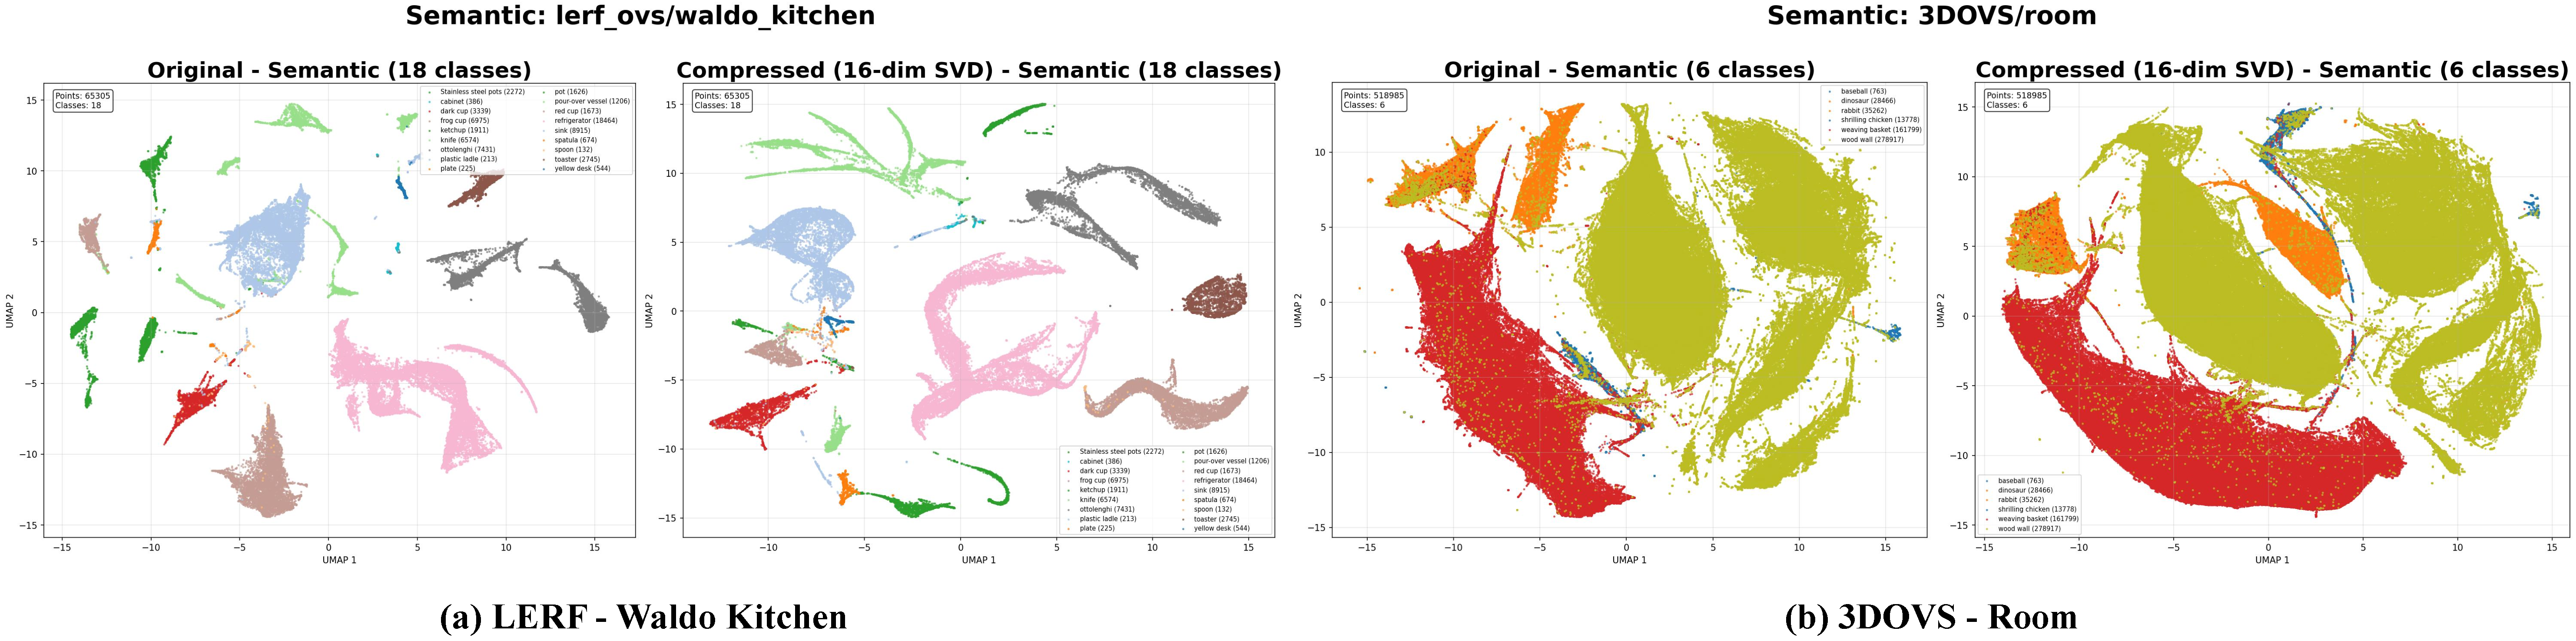
\includegraphics[width=\textwidth]{figs/JM-Visual.pdf}
  \caption{Visual comparison of feature distributions before and after dimensionality reduction in the feature space on the LERF and 3DOVS datasets.}
  \label{fig:JM-visual}
\end{figure}

\begin{table}[tb]
  \caption{Analysis of JM Distance. We present the JM distances computed under a Gaussian distribution assumption, as well as the JM distances obtained after aggregating the high‑dimensional distributions using arithmetic mean (AM) and geometric mean (GM). The compressed average JM distance actually shows an increasing trend.}
  \label{tab:jm-dist}
  \centering
  \resizebox{\textwidth}{!}{
  \begin{tabular}{@{}l|c|cccc|ccccc|c@{}}
    \toprule
    % 表头行：用 \multicolumn 覆盖竖线
    \multicolumn{1}{c}{\multirow{2}{*}{Setting}} & \multicolumn{1}{c}{\multirow{2}{*}{Metrics}} & \multicolumn{4}{c}{LERF} & \multicolumn{5}{c}{3D-OVS} & \multicolumn{1}{c}{\multirow{2}{*}{Avg}}\\
    \cmidrule(lr){3-6} \cmidrule(lr){7-11}
    \multicolumn{1}{c}{} & & Ramen & Figurines & Teatime & Kitchen & Bed & Bench & Room & Sofa & Lawn & \\
    \midrule
    & gaussian & 1.4128 & 1.4139 & 1.4110 & 1.4139 & 1.4142 & 1.4141 & 1.4142 & 1.4115 & 1.3875 & 1.4103\\
    origin & AM & 0.8061 & 0.9071 & 0.9522 & 0.9413 & 1.1786 & 1.0659 & 1.1303 & 1.1031 & 0.9342 & 1.0021\\
    & GM & 0.8506 & 0.9949 & 1.0322 & 1.0291 & 1.2492 & 1.1393 & 1.1987 & 1.1901 & 0.9702 & 1.0727\\
    \midrule
    & gaussian & 1.3887 & 1.4119 & 1.3994 & 1.4119 & 1.4142 & 1.4110 & 1.4137 & 1.4097 & 1.3013 & 1.3958($\textcolor{green}{-1.0\%}$)\\
    ours-16D & AM & 0.8992 & 1.0819 & 1.0661 & 1.1069 & 0.9475 & 1.0429 & 1.0045 & 1.0006 & 0.9539 & 1.0115($\textcolor{red}{+0.9\%}$)\\
    & GM & 0.9466 & 1.1829 & 1.1586 & 1.2319 & 1.1235 & 1.1397 & 1.1203 & 1.1649 & 0.9932 & 1.1179($\textcolor{red}{+4.2\%}$)\\
    \bottomrule
  \end{tabular}}
\end{table}

% 在这一节中，我们通过开放词汇场景领域常用的数据集，3DOVS与LERF数据集上的实验验证了SceneSplat-7k数据集中语言特征矩阵的低秩特性，并通过定量的方式验证了压缩后的特征空间的有效性。
In this section, we validate the low-rank property of the language feature matrix in the SceneSplat-7k \cite{li2025scenesplat} dataset through experiments on the commonly used open‑vocabulary scene datasets, namely 3DOVS \cite{liu2023weakly} and LERF\cite{lerf2023}, and quantitatively verify the effectiveness of the compressed feature space.

% 我们使用与SceneSplat相同的方法处理两个数据集，得到768维SigLIP2语言特征，并通过Occam's LGS聚合得到3D语言特征。随后，我们通过反投影的方式将2D标注映射到3DGS,并基于投票机制确定每个高斯的伪标签。我们使用UMap方法对原始特征空间和基于我们的方法压缩至16维的特征空间中各类别数据分布进行可视化，结果如图x所示。
% 压缩特征空间维度会细微影响各类别特征空间分布，但不影响类别间的可分性，原始高维空间中的不同簇在低维空间中亦不会重叠。
% Following the same procedure as in SceneSplat, we process both datasets to obtain 768‑dimensional SigLIP2 language features, which are then aggregated into 3D language features via Occam’s LGS \cite{cheng2024occamslgssimpleapproach}. The 2D annotations are subsequently back-projected onto the 3D Gaussians, and a voting mechanism is applied to assign pseudo‑labels to each Gaussian. We visualize the per‑class data distributions in the original feature space and in the 16‑dimensional feature space compressed by our method using UMAP, as shown in Figure \ref{fig:JM-visual}.
% While compressing the feature‑space dimension slightly alters the distribution of each class, it does not compromise inter‑class separability. The distinct clusters present in the original high‑dimensional space remain non‑overlapping after compression.
We follow SceneSplat’s procedure to process both datasets, extracting 768‑dim SigLIP2 \cite{tschannen2025siglip} language features and aggregating them into 3D language features via Occam’s LGS \cite{cheng2024occamslgssimpleapproach}. The 2D annotations are back‑projected onto 3D Gaussians, and a voting mechanism assigns pseudo‑labels to each Gaussian. In Figure \ref{fig:JM-visual}, we visualize the per‑class distributions in the original feature space and in our compressed 16‑dime space using UMAP.
Although feature‑space compression alters the within‑class distribution slightly, it preserves inter‑class separability: the distinct clusters observed in the original high‑dimensional space remain clearly separated after compression.

% 随后，我们使用JM距离对特征空间压缩前后各类别间的可分性进行定量分析。JM距离是一种衡量两个概率分布差异的距离度量，其值域为[0, √2]，值越大表示两类别的可分性越好。JM距离的定义基于巴氏距离，对于类别i,j，其概率分布$\tilde{p}_i(x)$与$\tilde{p}_j(x)}$间的巴氏距离为：
Subsequently, we employ the Jeffries-Matusita distance to quantitatively analyze the inter‑class separability before and after feature‑space compression. The JM distance, defined on the basis of the Bhattacharyya distance, measures the divergence between two probability distributions, ranging from 0 to $\sqrt{2}$, with larger values indicating better separability between two classes. The Bhattacharyya distance $B_{ij}$ between the probability distributions $\tilde{p}_i(x)$ and $\tilde{p}_j(x)$ is given by:
\begin{equation}
    B_{ij} = -\ln \left( \int \sqrt{\tilde{p}_i(x) \, \tilde{p}_j(x)} \, \mathrm{d}x \right)
\end{equation}
Hence, the JM distance between classes i and j is defined as $\text{JM}_{ij} = \sqrt{2(1 - e^{-B_{ij}})}$. We compute the average JM distance $\overline{\text{JM}}$ across all class pairs in a scene, where $c$ denotes the total number of classes.
\begin{equation}
    \overline{\text{JM}} = \frac{2}{c(c-1)} \sum_{i=1}^{c} \sum_{j>i}^{c} \sqrt{2(1 - e^{-B_{ij}})}
\end{equation}

% 实际计算过程中，需要先确定类别的分布以计算巴氏距离。当假设所有类别均为高斯分布时，类别i,j间的巴氏距离为：
To compute the Bhattacharyya distance in practice, the distribution of each class must first be estimated. Under the assumption that all classes follow Gaussian distributions, the Bhattacharyya distance between classes i and j is:
\begin{equation}
    B_{ij}^{\text{g}} = \frac{1}{8} (\mathbf{M}_i - \mathbf{M}_j)^T \left( \frac{\mathbf{V}_i + \mathbf{V}_j}{2} \right)^{-1} (\mathbf{M}_i - \mathbf{M}_j) + \frac{1}{2} \ln \left( \frac{ | \frac{\mathbf{V}_i + \mathbf{V}_j}{2} | }{ \sqrt{ | \mathbf{V}_i | \cdot | \mathbf{V}_j | } } \right)
\end{equation}
where $\mathbf{M}_i$ and $\mathbf{M}_j$ are the mean vectors of classes i and j, respectively, and $\mathbf{V}_i$ and $\mathbf{V}_j$ are their corresponding covariance matrices.
% 然而，所有类别不一定都满足高斯分布。同时，基于高斯分布假设计算JM距离时，高维特征的JM距离理论上大于低维特征，因为每个独立维度都为Bhattacharyya距离贡献非负值，产生累积的"维度红利"效应。因此，我们使用离散化方式计算任意分布间的JM距离。
% 具体而言，对每个维度的特征值进行离散化分箱统计得到各维度直方图，计算每维度的Bhattacharyya系数后通过算术/几何平均聚合，最后转换为JM距离。采用平均聚合的原因是各维度一般不满足相互独立，通过按维度平均的策略避免维度红利。基于算术和几何平均聚合的JM距离计算公式分别如Eq25,Eq26。
% However, not all classes necessarily follow Gaussian distributions. Moreover, when computing JM distances under the Gaussian assumption, the distance for high‑dimensional features is theoretically greater than that for low‑dimensional ones, because each independent dimension contributes a non‑negative value to the Bhattacharyya distance, resulting in a cumulative ``dimensional bonus'' effect. Therefore, we compute JM distances between arbitrary distributions using a discretization approach.
% Specifically, the feature values in each dimension are discretized into bins to obtain per‑dimensional histograms. The Bhattacharyya coefficient is computed for each dimension and then aggregated via arithmetic or geometric averaging, after which it is converted to  JM distance. Averaging across dimensions is adopted because the dimensions are generally not independent. This strategy avoids the dimensional bonus effect. 
Not all classes follow Gaussian distributions, and under the Gaussian assumption, high‑dimensional features obtain artificially inflated JM distances because each independent dimension adds a non‑negative contribution—a “dimensional‑bonus” effect. To avoid this, we compute JM distances via discretization. We bin the feature values in each dimension, compute the Bhattacharyya coefficient per dimension, aggregate the coefficients by arithmetic or geometric averaging, since dimensions are generally correlated, and finally convert the result to JM distance. This procedure makes no Gaussian or independence assumptions and eliminates the dimensional bonus.
The formulas for the JM distance based on arithmetic and geometric‑mean aggregation are given in Eq.\eqref{eq:jmam} and Eq.\eqref{eq:jmgm}, respectively.
\begin{equation}
    \text{JM}_{ij}^{\text{AM}} = \sqrt{2 \left(1 - \frac{1}{D} \sum_{d=1}^{D} \sum_{k=1}^{n_{b}} \sqrt{\tilde{p}_i(d,k) \cdot \tilde{p}_j(d,k)}\right)} 
    \label{eq:jmam}
\end{equation}
\begin{equation}
    \text{JM}_{ij}^{\text{GM}} = \sqrt{2 \left(1 - \exp\left(\frac{1}{D} \sum_{d=1}^{D} \ln\left(\sum_{k=1}^{n_{b}} \sqrt{\tilde{p}_i(d,k) \cdot \tilde{p}_j(d,k)}\right)\right)\right)}
    \label{eq:jmgm}
\end{equation}
where $n_b$ denotes the number of bins in the histogram, and $D$ indicates the feature dimensionality. 
% 各场景3种平均JM距离如表2所示。使用我们的方法压缩至16维的特征空间，其平均JM距离甚至整体高于原始特征空间，这证明了原始特征矩阵的冗余性。即使在高度压缩的低维空间中，不同类别特征分布间依然能保持良好的可分性，因此在不损失分类性能前提下进行降维是可能的。
The average JM distances across scenarios for different aggregation methods are presented in Table \ref{tab:jm-dist}. Our 16‑dimensionally compressed feature space yields an even higher average JM distance than the original space, confirming the redundancy of the original feature matrix. The distinct classes remain well‑separable in this low‑dimensional space, demonstrating that dimensionality reduction can be achieved without degrading classification performance.


\section{Details of Experimental Setup}
\label{sec:exp_details}

\subsection{Dataset Splits and Evaluation Details}

\noindent\textbf{SceneSplat-7k.} We evaluate our method on SceneSplat-7K, a large-scale indoor benchmark comprising 7,916 high-fidelity 3DGS scenes~\cite{dai2017scannet, yeshwanth2023scannet++, straub2019replica, roberts2021hypersim, wald20193rscan, dehghan2021arkitscenes, chang2017matterport3d}. Following its protocol, we pretrain on 4,114 scenes from ScanNet, ScanNet++ v2, and Matterport3D, and evaluate on their respective test sets across diverse object scales. We report average foreground IoU and accuracy.

\noindent\textbf{LERF-OVS.} Quantitative evaluations are conducted on the LERF-OVS dataset, which comprises everyday indoor scenes featuring diverse objects with pixel-wise semantic masks and paired short text queries. Adhering to the standard LERF evaluation protocol~\cite{lerf2023}, we focus on four representative scenes: Ramen, Figurines, Teatime, and Waldo Kitchen. Performance is assessed using two key metrics: mean IoU for open-vocabulary segmentation and localization accuracy.

% \noindent\textbf{LERF-MASK.} The LERF-Mask benchmark~\cite{ye2024gaussian}, a semantic subset of the original LERF dataset~\cite{lerf2023}, serves as the foundation for our evaluation. Comprising three indoor scenes (Figures, Ramen, and Teatime) annotated with 23 text prompts and 6--10 dense object masks per scene, this benchmark facilitates precise open-vocabulary segmentation assessment. Following~\cite{ye2024gaussian,lyu2024gaga}, we assess performance using mean Intersection over Union (mIoU) and boundary IoU (mBIoU).

% \noindent\textbf{3DOVS.} Evaluation of our method is also conducted on the 3D-OVS dataset \cite{liu2023weakly}, which features long-tail objects situated in diverse backgrounds. Following the protocol established in Occam's LGS \cite{cheng2024occamslgssimpleapproach}, we employ a dynamic thresholding strategy to identify and evaluate only stable regions. Quantitative assessment is conducted on five representative scenes: Sofa, Lawn, Bed, Room, and Bench. We utilize the ground-truth annotations provided by \cite{qin2024langsplat} to measure segmentation performance for these scenes.

% \noindent\textbf{Replica.}
% The Replica dataset~\cite{replica19arxiv} offers high-fidelity indoor reconstructions with dense geometry and comprehensive ground-truth annotations. Following the protocol in~\cite{Zhi:etal:ICCV2021,lyu2024gaga}, we select eight scenes and utilize their provided rendered imagery. For each scene, we uniformly split the data into 20\% for training and 20\% for testing, yielding 180 images per set. To evaluate the multi-view consistency of 3D segmentation masks, we leverage the dataset's ground-truth panoptic labels, disregarding specific class semantics.

% 我们的方法默认使用16-dim的特征进行训练，并报告指标。
\noindent\textbf{Note.} By default, our method employs \textbf{16-dim} features for training and reports the corresponding metrics.
\subsection{Implementation Details}
% SceneSplat使用PTv3作为基础模型进行基于3DGS的Vision-Language Pretraining。由于我们对特征进行了大幅度降维，因此可以使用更小，更轻量化的模型预测低维度的语言特征参数。我们使用LitePT作为基础模型，冻结其编码器并修改解码器架构以适配更低维度的输出。同时，我们也实现了一个基于PTv3的，仅修改解码器特征维度的版本。模型详细架构分别如表1和2所示，我们将在Sec.\ref{}进行详细消融实验。
SceneSplat employs PTv3 \cite{wu2024ptv3} as the backbone for 3DGS-based vision-language pretraining. Given our significant reduction in feature dimensionality, we can leverage smaller, more lightweight models to predict these low-dimensional language feature parameters. Specifically, we utilize LitePT \cite{yuelitept2026} as the backbone, freezing its encoder while modifying the decoder architecture to accommodate the lower-dimensional output. Additionally, we implement a variant based on PTv3 that modifies only the decoder's feature dimensionality. The detailed model architectures are presented in Table \ref{tab:litept} and \ref{tab:ptv3}, with comprehensive ablation studies provided in Section \ref{sec:ablation_details}.

We optimize all parameters of the 3D Gaussian primitives, including center position, color, opacity, quaternion rotation, and scale. The model is trained using the AdamW optimizer (initial learning rate $0.001$, weight decay $0.05$) coupled with a OneCycle scheduler featuring cosine annealing. Our objective function combines cosine similarity ($\lambda_{cos}=0.1$), L1 regularization ($\lambda_{L1}=1.0$), density consistency regularization ($\lambda_{dense}=1.0$)and contrastive loss ($\lambda_{con}=0.02$, temperature $\tau=0.2$). Notably, the contrastive loss is activated only during the final 75\% of the training process. To enhance robustness, we employ extensive data augmentation strategies, including random rotations, scaling, flipping, jittering, and elastic distortions.

% 我们使用4个RTX4090 GPU进行800轮data epochs训练。所有代码均基于PyTorch框架实现。
Training is conducted for 800 data epochs on four NVIDIA RTX 4090 GPUs. All inference experiments are conducted on a single NVIDIA RTX 4090. All implementations are built upon the PyTorch framework.

% 需要注意的是，针对2D评估标准，为了与SceneSplat方法进行公平比较，我们遵循官方提供的数据预处理流程基于训练视图提取768维度的siglip2-sam2语言特征，并统一进行10 epoch的微调。其余方法均使用512维CLIP特征，因此与我们的方法不能进行直接的比较，我们主要以SceneSplat为参考。
It is important to note that for the 2D evaluation metrics, we strictly adhere to the official data preprocessing pipeline of SceneSplat to ensure a fair comparison. Specifically, we extract 768-dimensional \textbf{SigLIP2-SAM2} language features from the training views. Since other baseline methods typically employ 512-dimensional CLIP features, direct comparison with them is not feasible due to the feature dimension mismatch. Consequently, our primary benchmark for evaluation is SceneSplat.

\begin{table}[htbp]
    \centering
    % PTv3
    \begin{minipage}[t]{0.5\textwidth}
    \caption{Model Configs for LitePT Vision-Language Pretraining.}
    \label{tab:litept}
    \resizebox{1\linewidth}{!}{
    \begin{tabular}{l|l}
    \toprule
    Config & Value \\
    \midrule
    embedding depth & 2 \\
    embedding channels & 32 \\
    encoder depth & [2, 2, 2, 6, 2] \\
    encoder channels & [36, 72, 144, 252, 504] \\
    encoder num heads & [2, 4, 8, 14, 28] \\
    encoder patch size & [1024, 1024, 1024, 1024, 1024] \\
    decoder depth & [2, 2, 2, 2] \\
    decoder channels & [16, 32, 64, 126] \\
    decoder num heads & [1, 2, 4, 7] \\
    decoder patch size & [1024, 1024, 1024, 1024] \\
    down stride & $[\times 2, \times 2, \times 2, \times 2, \times 2]$ \\
    mlp ratio & 2 \\
    qkv bias & True \\
    drop path & 0.3 \\
    \bottomrule
    \end{tabular}}
    \end{minipage}%
    \hfill%
    % 针对高维语言特征的不同适配与对齐方法在显存消耗与用时方面的对比。
    \begin{minipage}[t]{0.48\textwidth}%
    \caption{Model Configs for PTv3 Vision-Language Pretraining.}
    \label{tab:ptv3}
    \resizebox{1\linewidth}{!}{
    \begin{tabular}{l|l}
    \toprule
    Config & Value \\
    \midrule
    embedding depth & 2 \\
    embedding channels & 32 \\
    encoder depth & [2, 2, 2, 6] \\
    encoder channels & [32, 64, 128, 256] \\
    encoder num heads & [2, 4, 8, 16] \\
    encoder patch size & [1024, 1024, 1024, 1024] \\
    decoder depth & [2, 2, 2] \\
    decoder channels & [16, 64, 256] \\
    decoder num heads & [8, 8, 8] \\
    decoder patch size & [1024, 1024, 1024] \\
    down stride & $[\times 2, \times 2, \times 2, \times 2]$ \\
    mlp ratio & 2 \\
    qkv bias & True \\
    drop path & 0.3 \\
    \bottomrule
    \end{tabular}}
    \end{minipage}
\end{table}
% ---------------------------------------------------------------
% Section C: Additional Comparisons
% ---------------------------------------------------------------
% \section{Additional Comparison Results}
% \label{sec:add_comparisons}

\iffalse
\begin{table}[htbp]
\caption{Comparison of average IoU and F1 score on Replica Dataset.}
\begin{center}
\begin{tabular}{l|c|c|cc|c}
\toprule
Method & Venue & Type & mIoU(\%) & F-score (\%) & Time \\
\midrule
% LERF \cite{lerf2023} & ICCV'23 & Per-scene Optimization & 37.2 & 29.3 & >1h\\
% LangSplat \cite{qin2024langsplat} & CVPR'24 & Per-scene Optimization & 57.6 & 53.6 & >1h\\
Gaga \cite{lyu2024gaga} & Arxiv'24 & Semantic Clustering & 46.2 & 44.4 & 8min\\ %8.11min
GS-Grouping \cite{ye2024gaussian} & ECCV'24 & Semantic Clustering & 23.6 & 30.4 & >2h\\
OmniSeg3D-GS \cite{ying2023omniseg3d} & CVPR'24 & Per-scene Optimization & 39.1 & 35.9 & 20min\\ %20.35min
Unified-Lift \cite{zhu2025rethinking}& CVPR'25 & Per-scene Codebook & 41.6 & 43.9 & >2h\\

\midrule
SceneSplat* \cite{li2025scenesplat}& ICCV'25 & Generalizable & 40.1 & 40.3 & \underline{0.36min}\\
Ours & - & Generalizable & - & - & \textbf{0.06min}\\
\bottomrule
\end{tabular}
\label{tab: LERF}
\end{center}
\end{table}

\begin{table}[htbp]
\caption{Comparison of average IoU on 3D-OVS Dataset.}
\begin{center}
\resizebox{\textwidth}{!}{
\begin{tabular}{l|c|ccccc|c|c}
\toprule
Methods & Type & Bed & Bench & Room & Sofa & Lawn & Overall & Time\\
\midrule
% \specialrule{0.4pt}{0pt}{0pt} 
% LSeg & 56.0 & 6.0 & 19.2 & 4.5 & 17.5 & 20.6 \\
% LERF & 73.5 & 53.2 & 46.6 & 27.0 & 73.7 & 54.8 \\
GS-Grouping \cite{ye2024gaussian}& Semantic Clustering & 83.0 & 91.5 & 85.9 & 87.3 & 90.6 & 87.7 & >2h\\
Feature-3DGS \cite{zhou2024feature}& Per-scene Optimization & 83.5 & 90.7 & 84.7 & 86.9 & 93.4 & 87.8 & >3h\\
LEGaussians \cite{shi2024language}& Per-scene Optimization & 84.9 & 91.1 & 86.0 & 87.8 & 92.5 & 88.5 & >3h\\
GOI \cite{qu2024goi}& Per-scene Codebook & 89.4 & 92.8 & 91.3 & 85.6 & 94.1 & 90.6 & 45min\\
ILGS \cite{jsmbankILGS}& Per-scene Optimization & 96.4 & 95.5 & 93.6 & 92.2 & 94.2 & \underline{94.4} & 50min\\
LangSplat \cite{qin2024langsplat}& Per-scene Optimization & 92.5 & 94.2 & 94.1 & 90.0 & 96.1 & 93.4 & >1h\\
OccamLGS \cite{cheng2024occamslgssimpleapproach}& Per-scene Optimization-Free & 96.8 & 95.8 & 96.5 & 88.8 & 97.0 & \textbf{95.0} & 2min\\
\midrule
SceneSplat* \cite{li2025scenesplat}& Generalizable & 88.4 & 92.7 & 93.7 & 86.7 & 93.9 & 91.1 & \underline{0.22min}\\
Ours & Generalizable & 90.5 & 94.1 & 91.3 & 89.4 & 95.0 & 92.1 & \textbf{0.04min}\\
\bottomrule
\end{tabular}}
\label{tab: 3DOVS}
\end{center}
\end{table}
\fi

\iffalse
\begin{table}[tb]
  \centering
  \caption{Quantitative comparisons with generalized methods on [Dataset].}
  \label{tab:supp_comp_llff}
  \begin{tabular}{l c c c c}
    \toprule
    \textbf{Method} & \textbf{Setting} & \textbf{PSNR $\uparrow$} & \textbf{SSIM $\uparrow$} & \textbf{LPIPS $\downarrow$} \\
    \midrule
    Method A~\cite{RefA} & Pre-trained & 12.34 & 0.250 & 0.591 \\
    Method A~\cite{RefA} & Fine-tuned  & 17.07 & 0.436 & 0.529 \\
    Method B~\cite{RefB} & Pre-trained & 7.93  & 0.272 & 0.682 \\
    \textbf{Ours}        & \textbf{Sparse-view} & \textbf{20.45} & \textbf{0.712} & \textbf{0.196} \\
    \bottomrule
  \end{tabular}
\end{table}
\fi

% ---------------------------------------------------------------
% Section D: Ablation Studies Details
% ---------------------------------------------------------------
\section{Additional Ablation Results}
\label{sec:ablation_details}
\label{sec:extended-ablation}
\begin{table}[tb]
  \centering
  \caption{RPCA ablations on LERF.}
  \label{tab:ablation_latency}
  \begin{tabular}{@{}l|cc@{}}
    \toprule
    Method & Error & Latency \\
    \midrule
    RPCA-CPU & $6.28 \times 10^{-6}$ & >2h \\
    RPCA-GPU & $6.28 \times 10^{-6}$ & 330.55s \\
    Structured RPCA & $9.37 \times 10^{-3}$ & 0.18s \\
    \bottomrule
  \end{tabular}
\end{table}
\begin{table}[tb]
  \centering
  \caption{Ablation study on model architecture. We report the supervised semantic segmentation performance on ScanNet20.}
  \label{tab:ablation-arch}
  \begin{tabular}{c|cc|cc}
    \toprule
    \textbf{Model} &  mIoU(\%) & mAcc (\%) & Params(M) & Inference Time \\
    \midrule
    SceneSplat & 77.2 & 84.6 & 91.72 & 0.16min \\
    \midrule
    Ours-PTv3 & 77.2 & 84.5 & \underline{20.99} & \underline{0.05min} \\
    Ours-LitePT & 77.0 & 84.3 & \textbf{9.58} & \textbf{0.03min} \\
    \bottomrule
  \end{tabular}
\end{table}

We provide comprehensive ablation studies regarding efficiency, architectural choices and input
densities that could not be included in the main paper due to space constraints.

\subsection{Ablations on Model Architecture}
% 如表3所示，我们在ScanNet数据集上分别对LitePT与PTv3两种架构进行了有监督语义分割的性能评估。使用LitePT的版本相比PTv3版本在性能上不会有很大差距，却有着更小的参数量和更快的推理速度。虽然使用LitePT是最优选择，使用PTv3相比baseline依旧实现了4倍的参数量减小和3倍的推理加速。这说明了我们的语言特征压缩方法的有效性。
As shown in Table \ref{tab:ablation-arch}, we evaluate the supervised semantic segmentation performance of both LitePT and PTv3 architectures on the ScanNet dataset. The LitePT variant achieves performance comparable to PTv3, yet with significantly fewer parameters and faster inference speeds. While LitePT represents the optimal choice, the PTv3 variant still delivers a 4-fold reduction in parameters and a 3-fold acceleration in inference compared to the baseline. These results underscore the effectiveness of our language feature compression method.

\subsection{Ablations on input densities}
% 我们在ScanNet200上进行消融实验，以说明我们方法针对不同密度输入的鲁棒性。我们按照不同比例对原始3DGS进行下采样后输入模型，得到稀疏的3D语言特征，随后基于近邻投票策略进行0样本3D分割。随着采样率逐渐降低，整体性能成下降趋势，这是因为下采样一定程度上破坏了局部的几何结构和语义信息。而我们的Density Invariant learning策略相比不应用时在稀疏输入下有明显的性能提升，这说明了我们方法对稀疏输入的鲁棒性。
We conduct ablation studies on the ScanNet200 dataset in Table \ref{tab:sample-ablation} to demonstrate the robustness of our method against inputs of varying densities. Specifically, we downsample the original 3DGS at various ratios to generate sparse 3D language features, which are then processed via a nearest-neighbor voting strategy for zero-shot 3D segmentation.
In this paper, we set $K=3$, corresponding to the three sampling scenarios used in the density consistency loss: dense, half-density, and single-point-per-grid inputs.
As the sampling rate decreases, overall performance exhibits a downward trend, which is consistent with downsampling partially disrupting local geometric structures and semantic information. However, compared to the baseline without our Density-Invariant Learning strategy, our approach yields consistent improvements under sparse input conditions. The gains are modest at moderate compression levels but remain directionally stable across the sampling settings we evaluate, suggesting improved robustness when handling sparse data.


\begin{table}[htbp]
    \centering
    % Scannet 数据集上针对不同采样设置下，不同密度输入下性能的消融。
    \begin{minipage}[t]{0.5\textwidth}
    \caption{Ablation study on performance under different sampling settings and input densities on the ScanNet200 benchmark.}
    \label{tab:sample-ablation}
    \resizebox{1\linewidth}{!}{
    \begin{tabular}{c|cc|cc}
    \toprule
    \multirow{2}{*}{\textbf{Sample Rate}} & \multicolumn{2}{c}{with $\mathcal{L}_{dense}$} & \multicolumn{2}{c}{w/o $\mathcal{L}_{dense}$} \\
    \cmidrule(lr){2-3} \cmidrule(lr){4-5}
    & mIoU & mAcc & mIoU & mAcc \\
    \midrule
    30$\%$ & 18.0 & 30.6 & 16.0 & 29.1\\
    50$\%$ & 18.5 & 31.2 & 17.2 & 30.0\\
    70$\%$ & 18.8 & 31.7 & 18.0 & 30.7\\
    100$\%$ & 19.0 & 31.9 & 18.4 & 31.2\\
    \bottomrule
    \end{tabular}}
    \end{minipage}%
    \hfill%
    % 针对高维语言特征的不同适配与对齐方法在显存消耗与用时方面的对比。
    \begin{minipage}[t]{0.48\textwidth}%
      \caption{Comparison of memory consumption and runtime for different adaptation and alignment methods targeting high-dimensional language features.}
      \label{tab:efficiency}
      \resizebox{1\linewidth}{!}{
      \begin{tabular}{c|cc}
        \toprule
        \textbf{Method} & GPU Mem(MB) & Time \\
        \midrule
        Auto Encoder & 494 & 1h \\
        \midrule
        Ours-8dim & \textbf{165} & \textbf{5.7ms} \\
        Ours-16dim & \underline{297}& \underline{8.4ms} \\
        Ours-32dim & 563 & 14.5ms \\
        \bottomrule
      \end{tabular}}
    \end{minipage}
\end{table}

% 不同维度空间对齐方法的效率比较 Dimensional Space
\subsection{Efficiency Comparison of Different Alignment Methods}
% 以往基于CLIP等2D预训练模型的方法，在对原始高维语言特征进行降维时，不可避免的需要依赖每个场景训练一个Auto Encoder，以压缩和恢复特征，这个过程十分漫长。而我们的Orthogonal Procrustes Analysis方法仅需求解一个低维的变换矩阵，便可直接将高维文本嵌入与低维特征对齐。具体计算与存储开销见表5，我们的方法每场景仅需毫秒级别的开销，相比Auto Encoder快了6个数量级，同时占用更少内存。使用我们的方法可以几乎无损耗的在低维空间实现推理，使实时的3D开放词汇感知与场景理解成为可能。
Previous methods \cite{cheng2024occamslgssimpleapproach, qin2024langsplat, li2025langsplatv2} based on 2D pre-trained models like CLIP \cite{DBLP:journals/corr/abs-2103-00020} often require training a scene-specific autoencoder to compress and reconstruct high-dimensional language features during dimensionality reduction. In contrast, our Orthogonal Procrustes Analysis approach only requires solving for a low-dimensional transformation matrix to directly align high-dimensional text embeddings with low-dimensional features.
As detailed in Table \ref{tab:efficiency}, our method incurs millisecond-level overhead per scene and consumes less memory than the autoencoder-based alternative. This alignment cost is incurred only at query time, whereas constructing SceneSplat-Compact itself is a one-time offline preprocessing step that can be amortized across repeated downstream runs. The result makes low-dimensional inference practical without the per-scene optimization burden of autoencoder-based reduction.


% ---------------------------------------------------------------
% Section E: Visualizations
% ---------------------------------------------------------------
\section{Additional Visualization Results}
\label{sec:add_vis}

\subsection{Comparison with SOTA Methods}
% 图1展示了我们方法在3DOVS与Replica数据集上的零样本开放词汇物体定位与实例分割的结果。我们的方法与SceneSplat有着相当的泛化性能。
Figure \ref{fig:SuppVisualize} illustrates the results of our method for zero-shot open-vocabulary object localization and instance segmentation on the 3DOVS\cite{liu2023weakly} and Replica\cite{straub2019replica} datasets. Our approach demonstrates comparable generalization performance to SceneSplat.

\subsection{Visualizations of Our Method}
% 图2展示了Scannet数据集上特征图在降维前后的PCA可视化对比。降维前后基本不损失空间和语义信息，只是在可视化的时候存在颜色差异，这是由PCA本身的性质决定的。
Figure \ref{fig:Visualize-Compare} presents a PCA visualization comparison of feature maps on the ScanNet dataset before and after dimensionality reduction. The low-dimensional representation preserves most of the large-scale spatial and semantic structure, although some fine-grained boundaries and closely related categories become less distinct. The observed color discrepancies in the visualization are also affected by the nature of PCA itself.

\begin{figure}[tb]
  \centering
  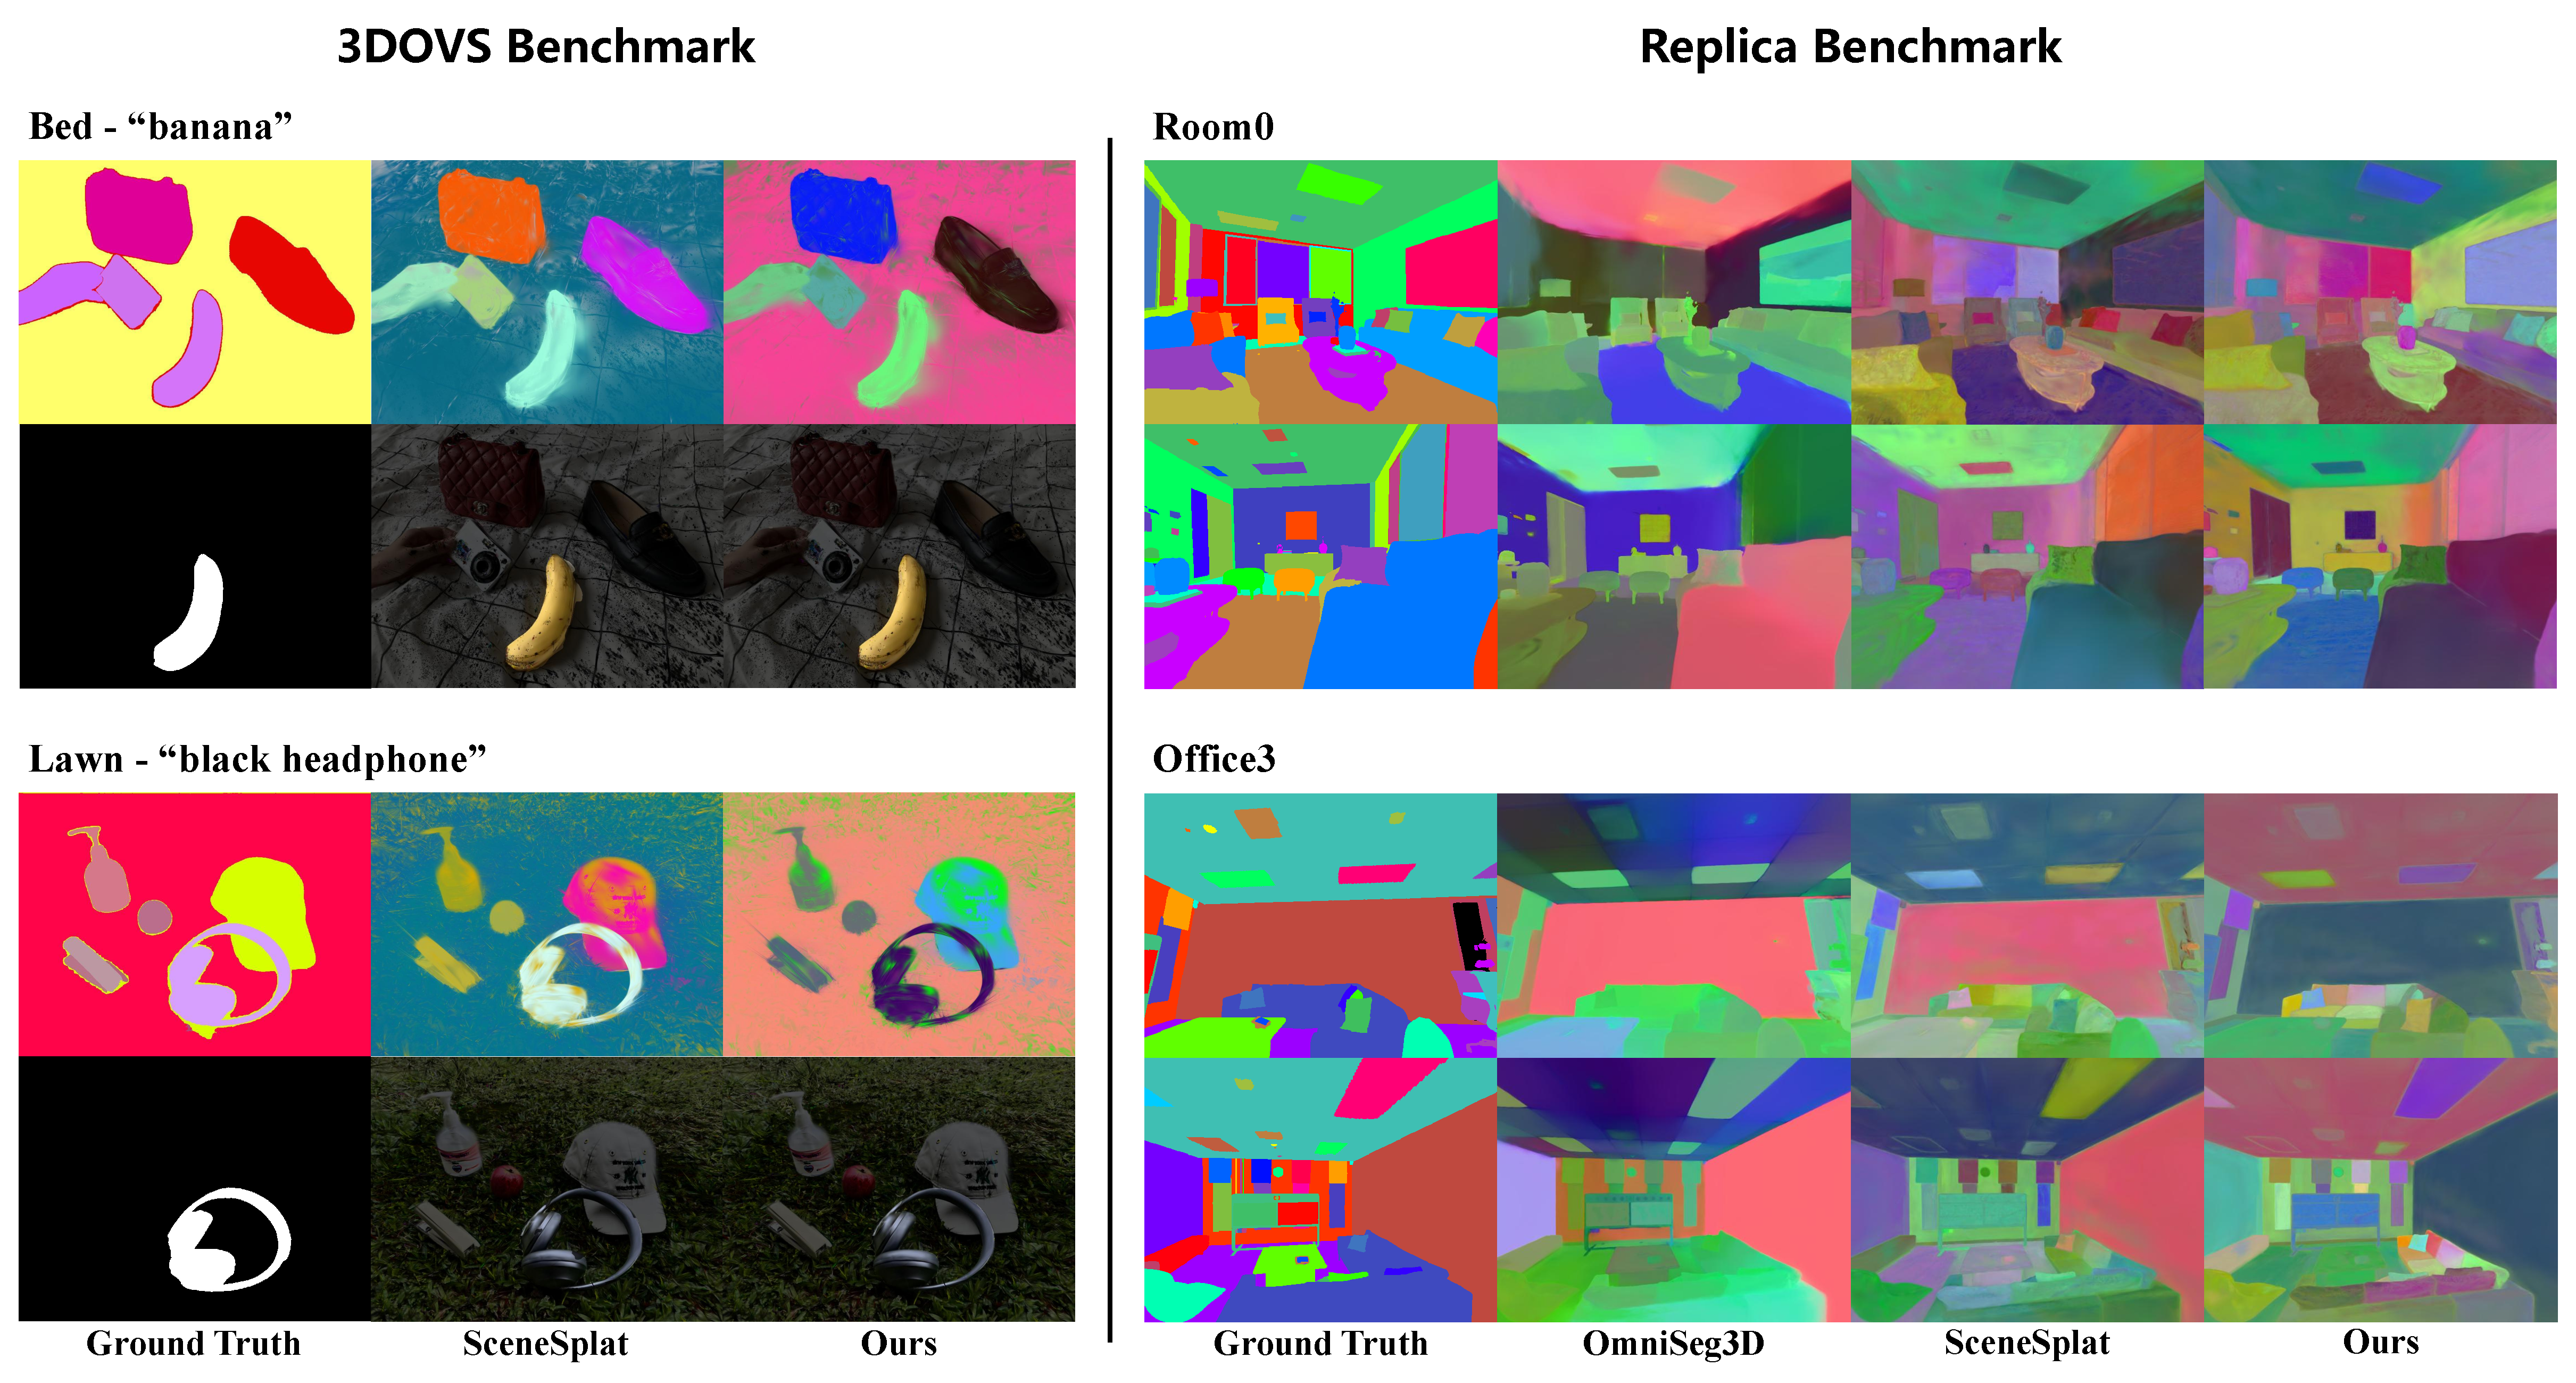
\includegraphics[width=\textwidth]{figs/Replica-3DOVS.pdf}
  \caption{Visualization of open-vocabulary recognition and object query results on the 3DOVS \& Replica datasets. Our model demonstrates strong generalization capabilities.}
  \label{fig:SuppVisualize}
\end{figure}

% ---------------------------------------------------------------
% Section F: Future Work
% ---------------------------------------------------------------
\section{Discussion, Limitations, and Future Work}
\label{sec:future}
While our compression pipeline achieves substantial storage reduction and fast inference, we observe several important limitations. First, optimizing models in the compressed low-dimensional space is more difficult than in the original high-dimensional setting: convergence is slower, sensitivity to hyperparameters is higher, and the simplified representation may blur difficult boundaries or fine-grained categories. This suggests that the current linear projection, while efficient for alignment and deployment, does not fully preserve the optimization geometry of the original feature space.

Second, our empirical study is centered on the storage bottleneck caused by large precomputed language features in SceneSplat-style pipelines. Although the underlying ideas may transfer more broadly, the paper does not claim universal gains across all 3D open-vocabulary representations, feature encoders, or training recipes. Third, the strongest benefit of our method is efficiency; under aggressive compression, absolute accuracy can still lag behind heavier methods that optimize directly in the original feature space. Finally, we do not exhaustively ablate the grid size used in spatial aggregation. This parameter controls a trade-off between stronger compression and better preservation of boundaries, small objects, and rare categories, and a more systematic sensitivity study is left to future work.

Future work will focus on discovering more training-friendly low-dimensional feature transformations. We also plan to report the end-to-end cost of constructing SceneSplat-Compact more systematically at larger scales and to study stronger baselines for feature extraction-time compression. In addition, we will investigate learnable non-linear mapping functions or adaptive basis expansions that can better preserve the optimization geometry of the original features while maintaining compactness. Exploring network architectures specifically tailored for low-dimensional feature training could further mitigate the difficulty of optimization in compressed spaces. By designing structures that better align with the geometric properties of the reduced latent space, we aim to ultimately bridge the gap between extreme compression efficiency and training stability.

\begin{figure}[tb]
  \centering
  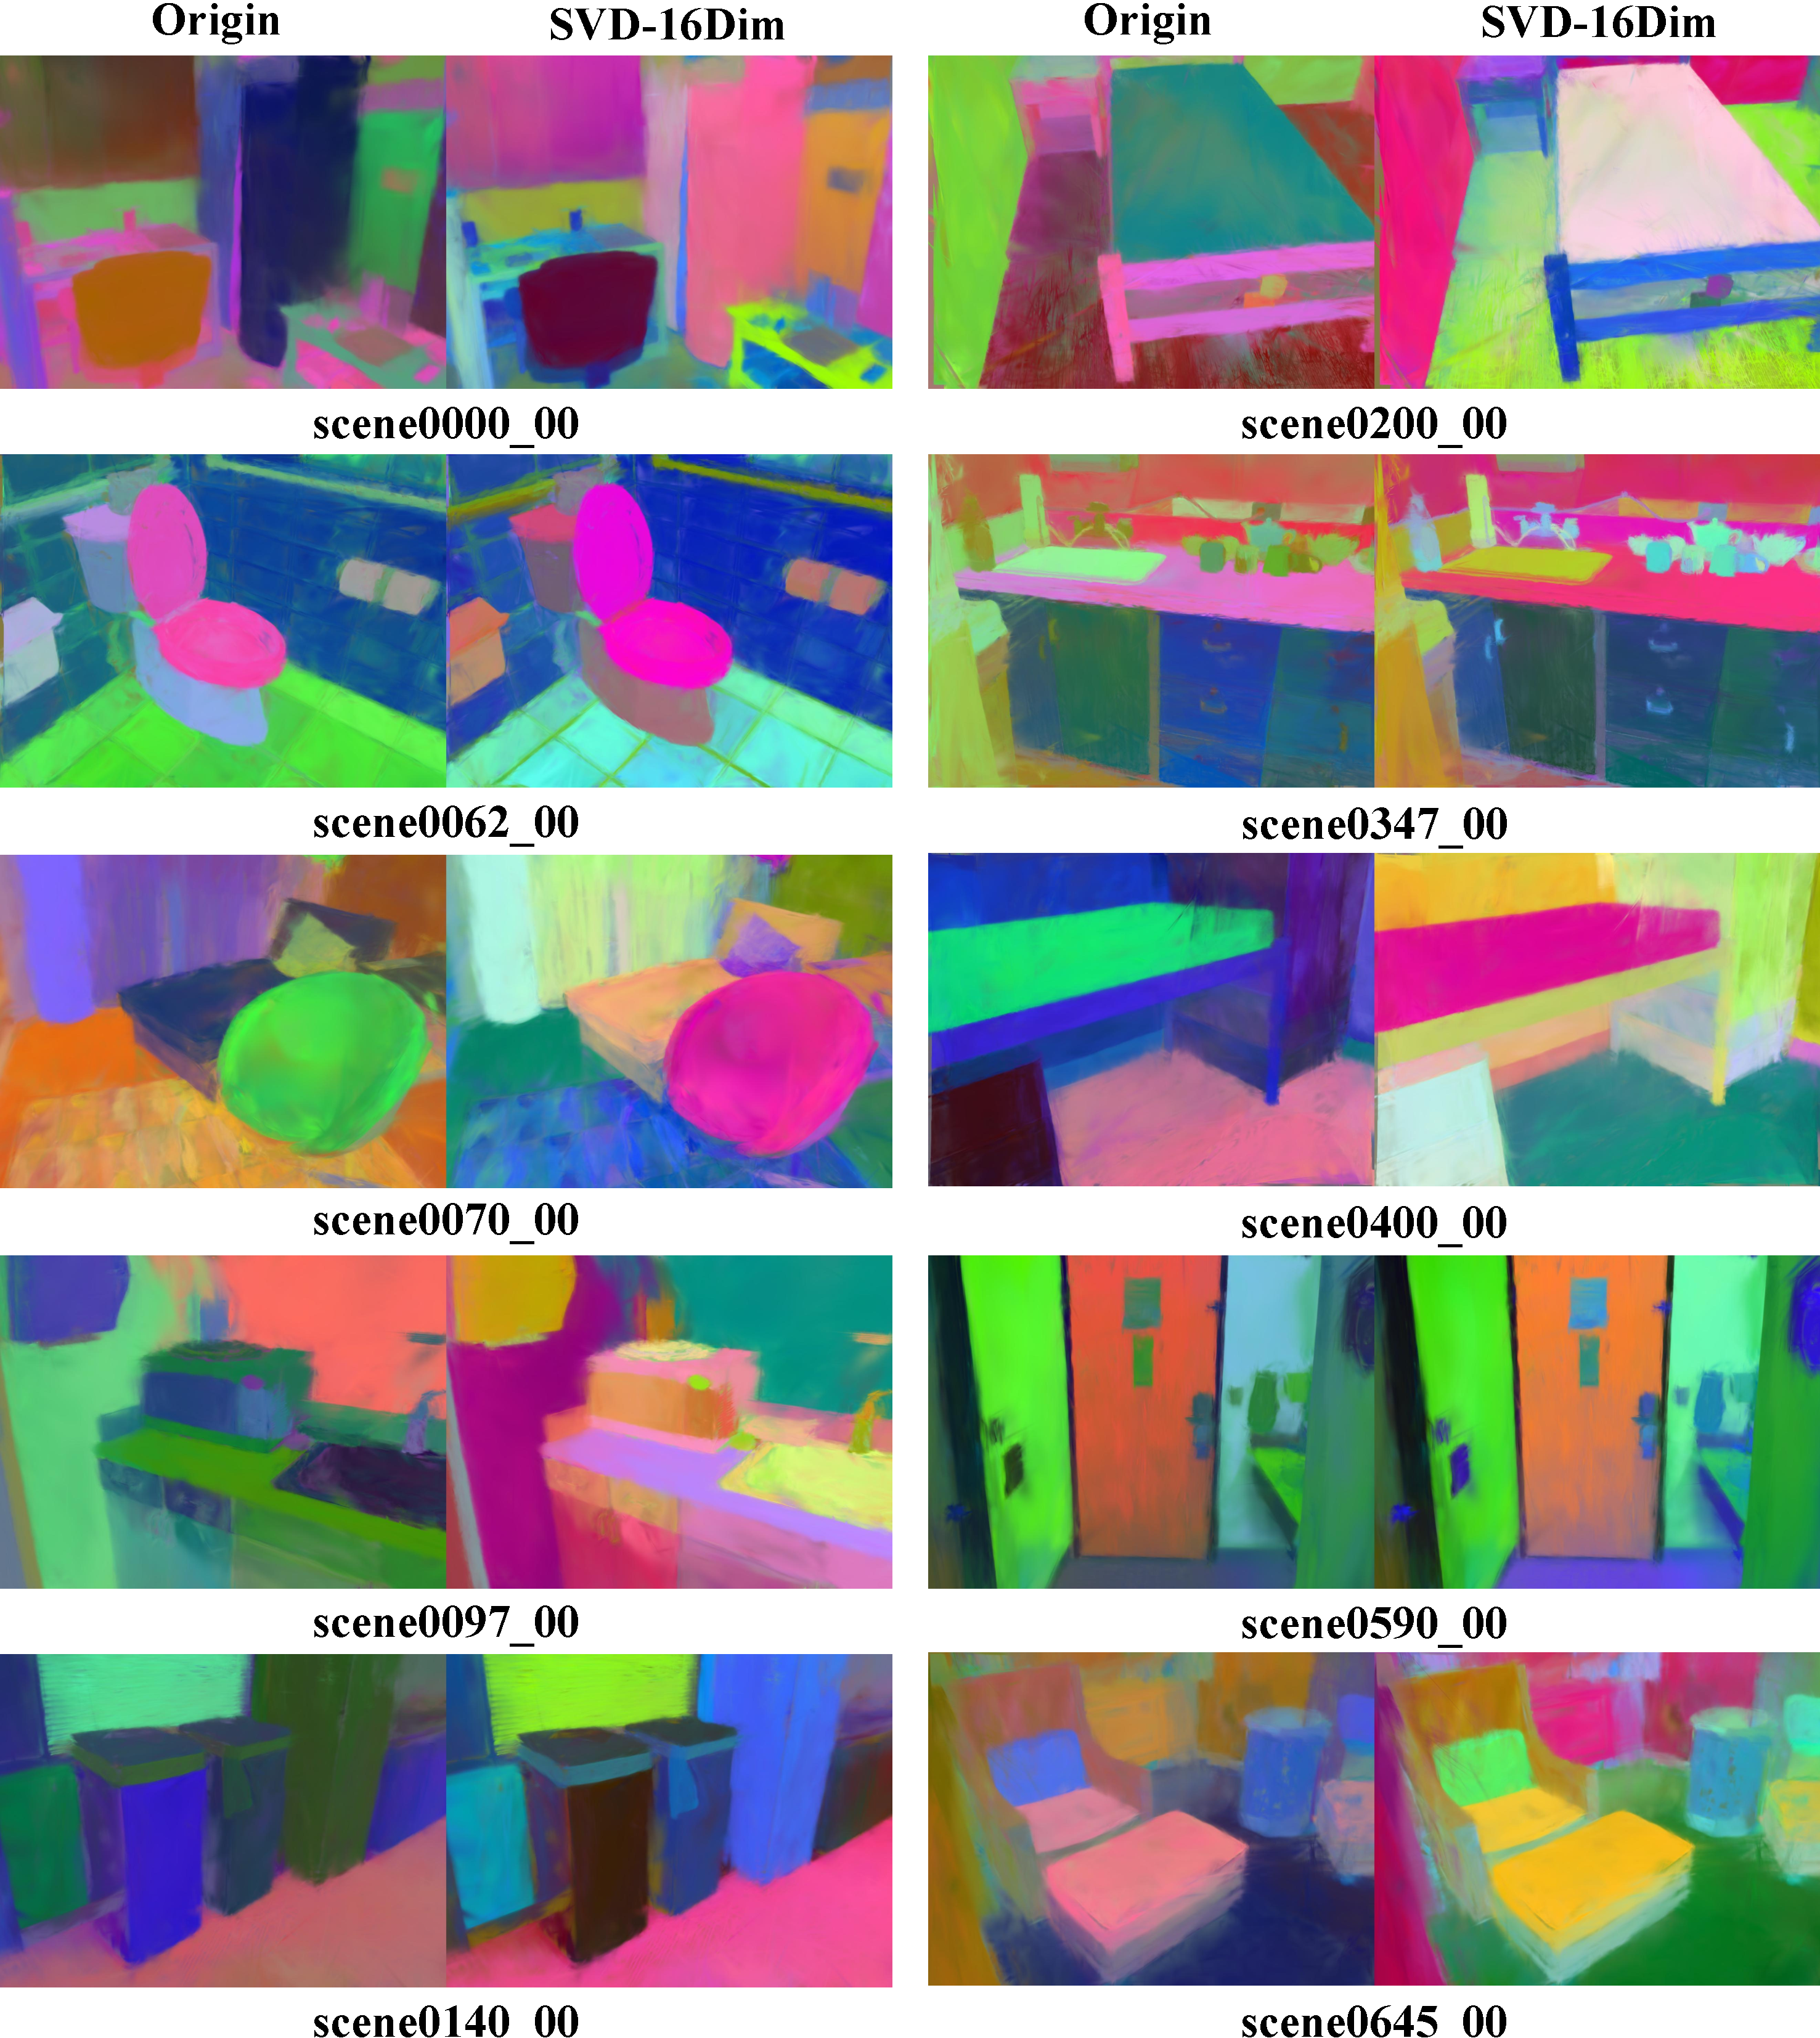
\includegraphics[width=\textwidth]{figs/SVDCompare.pdf}
  \caption{Visual comparison of feature maps on the ScanNet dataset before and after feature compression. Our method effectively preserves the original semantic information, although slight visual discrepancies exist compared to the original feature maps.}
  \label{fig:Visualize-Compare}
\end{figure}

% ---------------------------------------------------------------
% Bibliography
% ---------------------------------------------------------------
% Note: Usually supplementary material cites the same bib file as the main paper.
% Ensure your .bib file contains all references cited here.

\end{document}
